\chapter{Diseño del sistema.}
\label{cap: capitulo_4}

En este capítulo vamos a detallar cómo hemos concebido la solución a los requisitos \textit{software}, teniendo en cuenta los correspondientes al \textit{hardware} y a partir de los elementos que hemos descrito en el capítulo anterior.

\section{Planteamiento}

Como idea más abstracta, el \textit{software} que tenemos que diseñar consiste en un reproductor de archivos \acrshort{MIDI}, que recibe el fichero y lo envía a la \acrshort{PCB} a través del \acrshort{GPIO}. Por supuesto, la reproducción estará controlada por el usuario:

\smallskip

\begin{figure}[H]
	\noindent \begin{centering}
		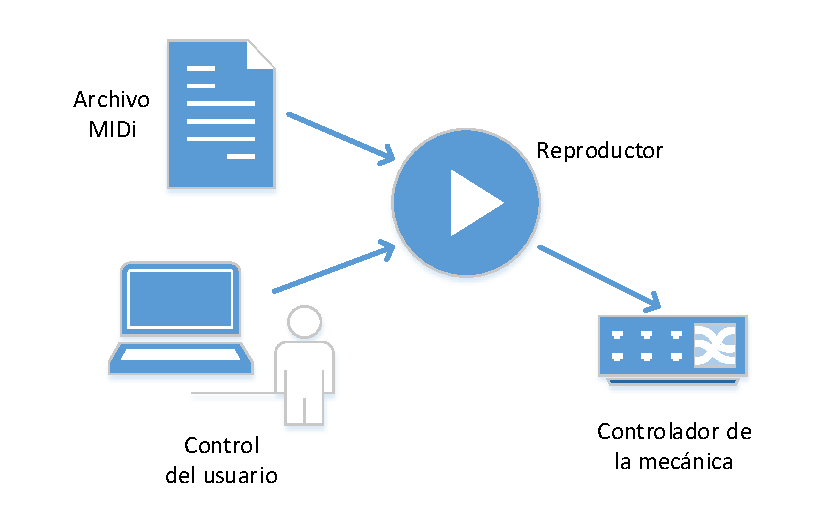
\includegraphics[width=\linewidth/2]{capitulo4/idea}
		\par\end{centering}
	\smallskip
	\caption{\label{fig:idea} Planteamiento inicial.}
\end{figure} 

\smallskip

Luego, dividiremos el sistema en cuatro grandes bloques. Respecto al de control, se requiere varias formas de acceder al sistema:

\begin{enumerate}
	\item Un \textit{software} controlador principal, que cubra todos los casos de uso, y sea fácil de instalar y utilizar, con preferencia de que sea multiplataforma.
	
	\item Un mando a distancia, que altere la reproducción.
	
	\item Un control reducido empotrado en la \acrshort{PCB}.
\end{enumerate}

Atendiendo a los requisitos del primer controlador y a las prestaciones del \textit{Raspberry Pi}, y con objeto de eliminar la necesidad de instalar y mantener aplicaciones en otro sistema, decidimos enfocar la solución como una interfaz \textit{web} con un servidor alojado en el \textit{Raspberry Pi}. De esta forma podemos llegar fácilmente a cualquier sistema operativo de escritorio, incluso es fácilmente adaptable a dispositivos móviles.

Sin embargo, el reproductor no puede funcionar dentro de un servidor \textit{web}, ya que éstos atienden peticiones sin estado, y se cierran automáticamente después de devolver la información. Por ello, vamos a diseñar el reproductor como un \textit{demonio} de Linux, junto con sus módulos auxiliares.

En último lugar, necesitamos almacenar información de los archivos \acrshort{MIDI}, listas de reproducción y asignaciones del mando en memoria persistente. Una base de datos nos permitiría guardar toda esa información de manera estructurada y coherente, además de ser fácilmente accesible por todos los componentes del sistema.

\section{Demonio del reproductor}

Un demonio ---\textit{daemon}--- es un proceso que se ejecuta en segundo plano en la fase de arranque del sistema operativo, y no interactúa directamente con el usuario, sino que se comunica con otros procesos a través de herramientas proporcionadas por el sistema operativo. \cite{wiki_demonio}

Este programa será el núcleo de nuestro sistema, y ofrecerá las siguientes vías para comunicarse:

\begin{enumerate}
	\item Un \textit{socket} local de Linux. Será usado principalmente por la interfaz \textit{web}, pero es una forma flexible y eficiente para que lo hagan más aplicaciones.
	
	\item El puerto en serie (\acrshort{UART}) del \textit{Raspberry Pi}, para recibir órdenes del mando.
	
	\item Los pines del \acrshort{GPIO} correspondientes al codificador rotatorio y el \acrshort{LCD}, para la interfaz reducida.
\end{enumerate}

Así, el esquema de uso de los distintos componentes queda así:

\smallskip

\begin{figure}[H]
	\noindent \begin{centering}
		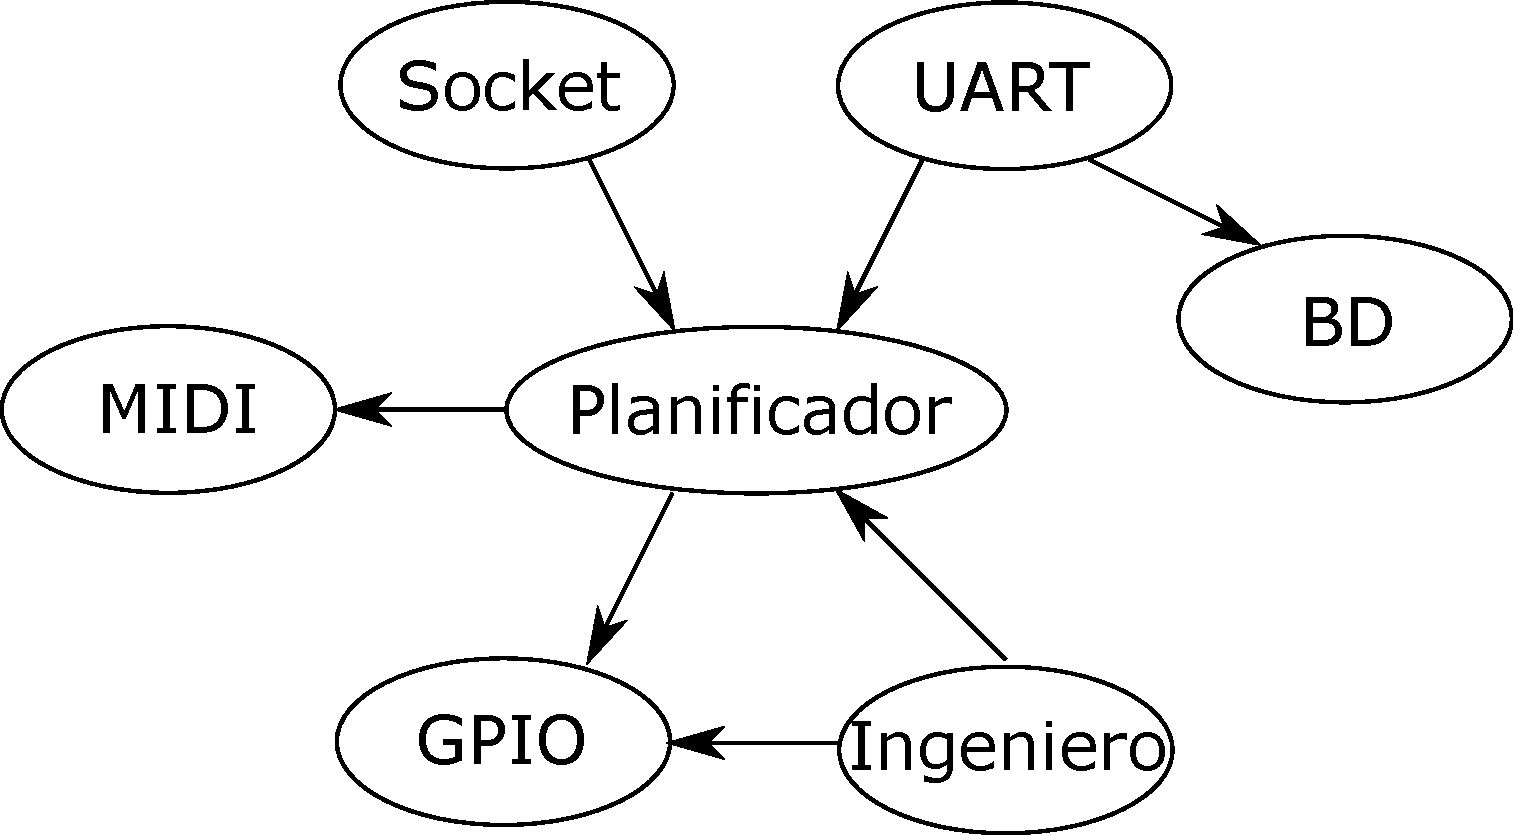
\includegraphics[width=\linewidth/2]{capitulo4/daemon}
		\par\end{centering}
	\smallskip
	\caption{\label{fig:daemon} Diagrama de uso entre los componentes del reproductor.}
\end{figure} 

\smallskip

\subsection{Descodificador de MIDI}
\label{subsec:daemon_midi}

Como hemos detallado más arriba, el formato \acrshort{MIDI} expone los eventos de control en orden temporal, clasificados por pistas, habitualmente simultáneas. Debemos proporcionar una estructura de datos que permita mantener cada archivo a reproducir en memoria y facilitar el acceso individual a cada pista.

Concebimos la estructura de datos principal como un conjunto de pistas, compuestas a su vez de eventos. El tamaño de los eventos normales es constante, sin embargo, los meta-eventos extienden la semántica con una cadena de datos.

El siguiente diagrama de clases ilustra la estructura de datos completa:

\smallskip

\begin{figure}[H]
	\noindent \begin{centering}
		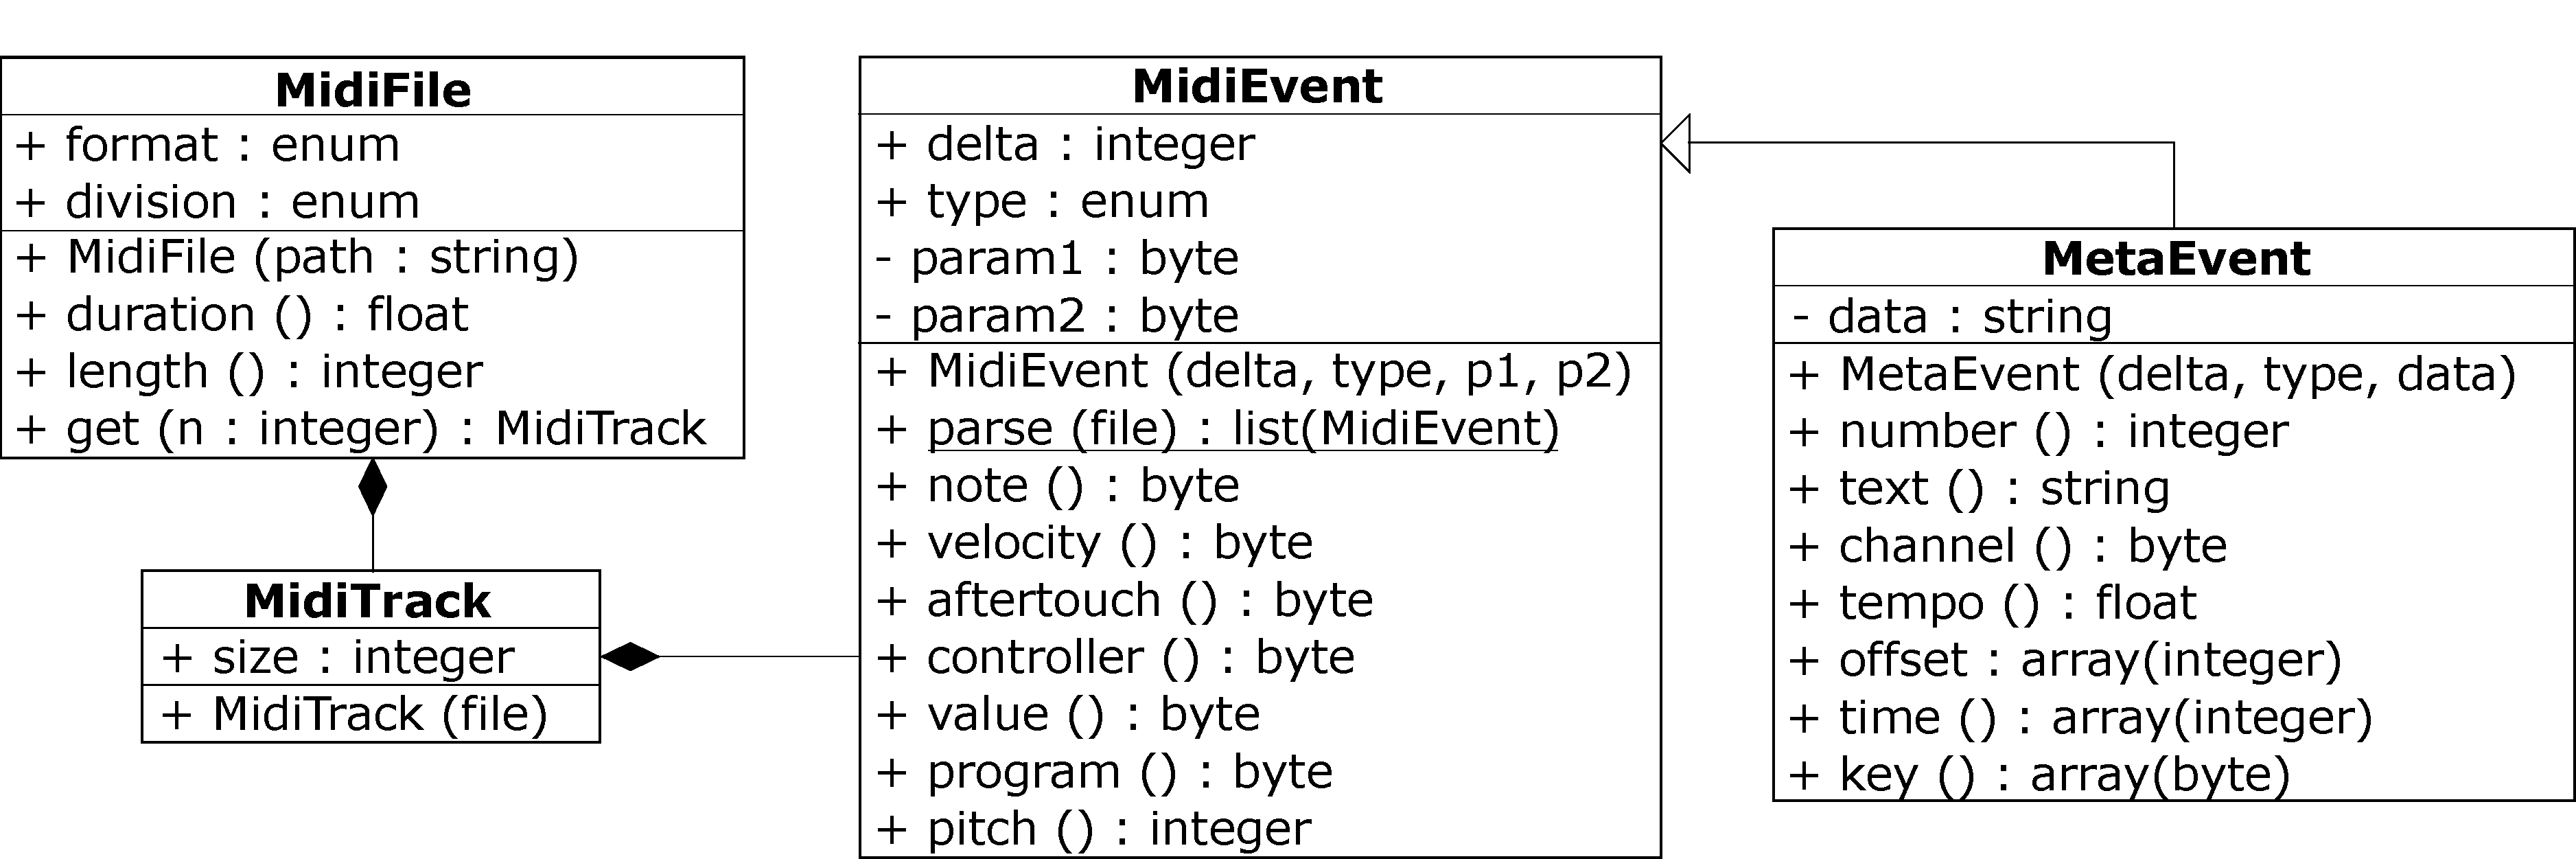
\includegraphics[width=\linewidth*3/4]{capitulo4/uml_midi}
		\par\end{centering}
	\smallskip
	\caption{\label{fig:uml_midi} Diagrama de clases para el módulo MIDI.}
\end{figure} 

\smallskip

\subsubsection{Clase MidiFile}

Define un archivo \acrshort{MIDI}. Sus atributos son:

\begin{description}
	\item[format : \textit{enum}] Formato del archivo. Puede tener los siguientes valores enumerados:
	
	\begin{description}
		\item[SINGLE\_TRACK] Una sola pista.
		\item[MULTIPLE\_SIMULTANEOUS] Varias pistas, simultáneas.
		\item[MULTIPLE\_INDEPENDENT] Varias pistas, independientes.
	\end{description}
	
	\item[division : \textit{enum}] Unidad de medida de la división de tiempo:
	
	\begin{description}
		\item[TICKS\ PER\ BEAT] La división se especifica en \textit{ticks}/\quarternote.
		\item[FRAMES\_PER\_SECOND] La división se especifica en \textit{ticks/fotograma}.
	\end{description}

\end{description}

La clase declara los siguientes métodos:

\begin{description}[style=nextline]
	\item[MidiFile (path)] 
	Constructor, lee un archivo \acrshort{MIDI}. 
	
	\begin{description}
		\item[path : \textit{string}] Ruta del fichero a leer.
	\end{description}
	
	\item[duration () : \textit{float}] 
	Obtener la duración de una pieza en segundos.
	
	\item[length : \textit{integer}]
	Devuelve el número de pistas contenidas en el archivo.
	
	\item[get (n) : \textit{MidiFile}]
	Devuelve la pista indicada.
	
	\begin{description}
		\item[n : \textit{integer}] Índice de pista.
	\end{description}
\end{description}

\subsubsection{Clase MidiTrack}

Esta clase se modela como una colección de los eventos pertenecientes a cada pista de un archivo \aceshort{MIDI}.

Solo contiene un atributo intrínseco y un constructor:

\begin{description}
	\item[size : \textit{integer}] Tamaño en \textit{bytes} que ocupa la pista en el fichero.
\end{description}

\begin{description}
	\item[MidiTrack (file)]
	Construye una pista a partir de un fichero abierto.
	
	\begin{description}
		\item[file] Archivo \acrshort{MIDI} abierto. Su tipo depende del sistema subyacente.
	\end{description}
\end{description}

\subsubsection{Clase MidiEvent}

Define un evento \acrshort{MIDI}.

\begin{description}
	\item[delta : \textit{integer}] Separación temporal respecto al evento anterior.
	\item[type : \textit{enum}] Tipo de evento. Se enumeran en la tabla \ref{tab:midi_eventos}.
	\item[param1 : \textit{byte}] Valor del primer parámetro, dependiendo del tipo de evento.
	\item[param2 : \textit{byte}] Valor del segundo parámetro, dependiendo del tipo de evento.
\end{description}

Los parámetros se consideran privados, ya que su semántica depende del tipo de evento. Por tanto, estableceremos los siguientes métodos para obtener la información adecuada:

\begin{description}[style=nextline]
	\item[MidiEvent (delta, type, p1, p2)]
	Crea un nuevo evento.
	
	\begin{description}
		\item[delta : \textit{integer}] Separación temporal respecto al evento precedente.
		\item[type : \textit{enum}] Tipo de evento.
		\item[p1 : \textit{byte}] Valor del primer parámetro.
		\item[p2 : \textit{byte}] Valor del segundo parámetro.
	\end{description}
	
	\item[parse (file) : \textit{list(MidiEvent)}]
	Analiza un archivo \acrshort{MIDI} en el punto en que estaba abierto, hasta encontrar un evento de final de pista.
	
	\begin{description}
		\item[file] Archivo \acrshort{MIDI} abierto. Su tipo depende del sistema subyacente.
	\end{description}
	
	Devuelve una lista de eventos.
	
	\item[note () : \textit{byte}] 
	Código de nota musical.
	
	\item[velocity () : \textit{byte}] 
	Velocidad de pulsación (intensidad del sonido).
	
	\item[aftertouch () : \textit{byte}] 
	Variación de intensidad.
	
	\item[controller () : \textit{byte}] 
	Número de controlador.
	
	\item[value () : \textit{byte}] 
	Valor del controlador.
	
	\item[program () : \textit{byte}] 
	Número de programa.
	
	\item[pitch () : \textit{byte}] 
	Valor del \textit{pitch-bend}.
\end{description}

\subsubsection{Clase MetaEvent}

Define un meta-evento. Extiende la clase \textit{MidiEvent} y presenta un atributo privado:

\begin{description}
	\item[data : \textit{string}] Cadena de datos correspondientes al meta-evento.
\end{description}

Podemos interactuar con el meta-evento mediante los siguientes métodos, cada uno será válido para el tipo de meta-evento que corresponda.

\begin{description}[style=nextline]
	\item[MetaEvent (delta, type, data)]
	Crea un nuevo meta-evento.
	
	\begin{description}
		\item[delta : \textit{integer}] Separación temporal respecto al evento precedente.
		\item[type : \textit{enum}] Tipo de evento.
		\item[data : string] Cadena de datos correspondientes al meta-evento.
	\end{description}
	
	\item[number () : \textit{integer}] 
	Número de secuencia.
	
	\item[text () : \textit{string}] 
	Texto del meta-evento.
	
	\item[channel () : \textit{byte}] 
	Devuelve el canal por defecto.
	
	\item[tempo () : \textit{float}] 
	Velocidad de ejecución del pasaje musical, en \textit{$\mu s / \quarternote$}.
	
	\item[offset () : \textit{array(integer)}] 
	Desplazamiento temporal. Devuelve una tupla con el siguiente contenido:
	
	\begin{enumerate}
		\item Velocidad en \textit{cuadros / s}.
		\item Hora.
		\item Minuto.
		\item Segundo.
		\item Cuadro (\textit{frame}).
	\end{enumerate}
	
	\item[time () : \textit{array(integer)}] 
	Devuelve la marca de compás mediante una tupla de la siguiente manera:
	
	\begin{enumerate}
		\item Numerador.
		\item Denominador como fracción de redonda. (\fullnote =1, \halfnote = 2, \quarternote =4, \eighthnote =8 ...)
 		\item Número de \textit{ticks} entre cada marca del metrónomo.
 		\item Subdivisión, en \textit{fusas / click}.
	\end{enumerate}
	
	\item[key () : \textit{array(integer)}] 
	Devuelve la tonalidad de la pieza, mediante una tupla con el siguiente significado:
	
	\begin{enumerate}
		\item Número de $\sharp$ si es positivo, o número de $\flat$ si es negativo.
		\item Modo, de forma enumerada:
		
		\begin{description}
			\item[MAJOR] Modo mayor.
			\item[MINOR] Modo menor.
		\end{description}
	\end{enumerate}
\end{description}

\subsubsection{Diagrama de uso}

El módulo \acrshort{MIDI} solo se usa directamente a través del planificador. Éste se encarga de gestionar las partituras, y ordenar su eliminación cuando sea necesario.

\smallskip

\begin{figure}[H]
	\noindent \begin{centering}
		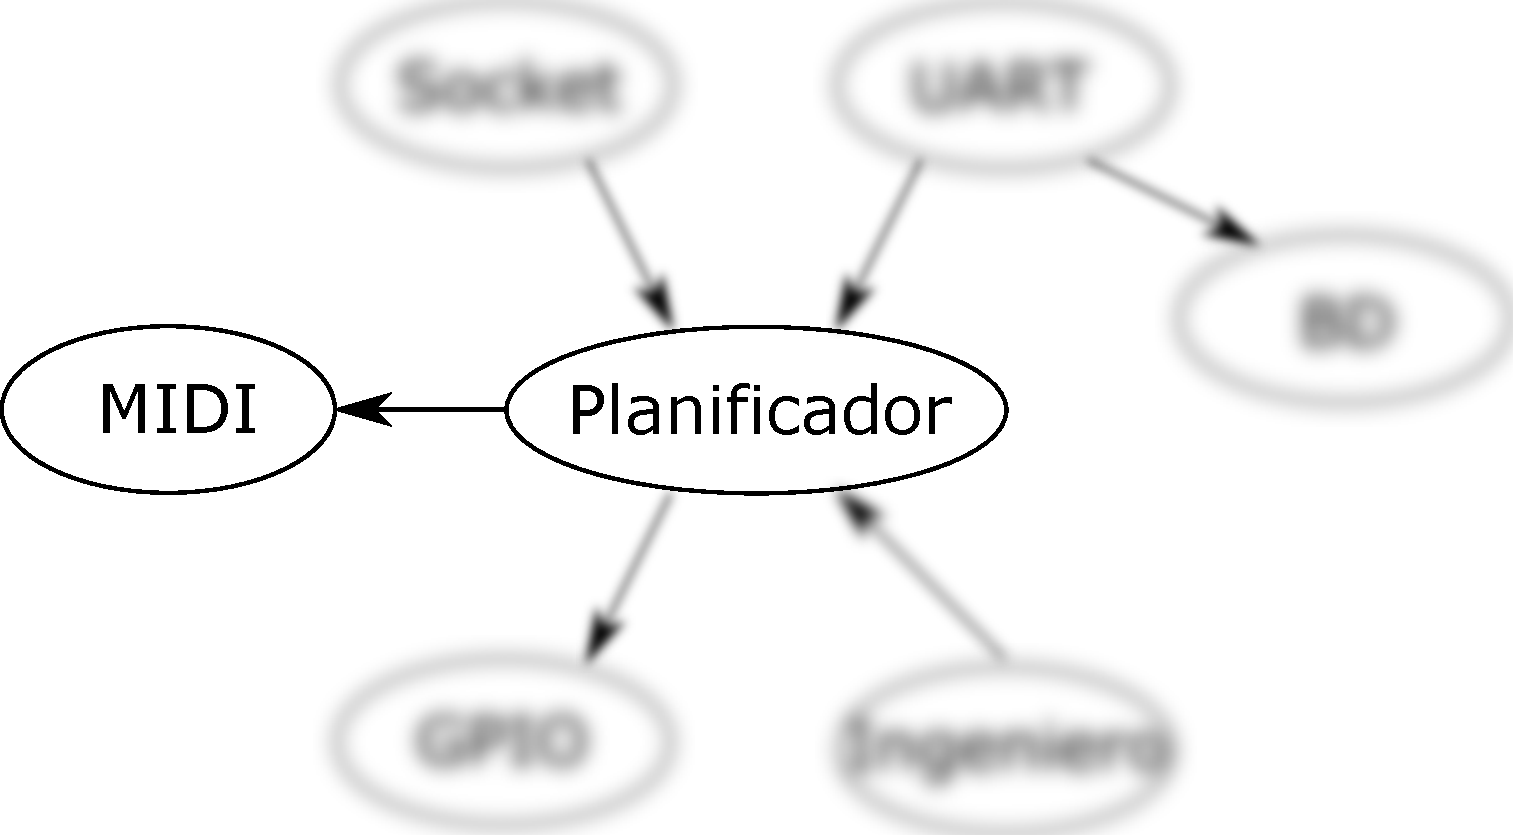
\includegraphics[width=\linewidth/2]{capitulo4/daemon_midi}
		\par\end{centering}
	\smallskip
	\caption{\label{fig:daemon_midi} Diagrama de uso del módulo MIDI.}
\end{figure} 

\smallskip

\subsection{Control por socket}
\label{subsec:daemon}

Un \textit{socket} un mecanismo de comunicación inter-proceso ---\acrshort{IPC} (\textit{\acrlong{IPC}})--- que proporciona Linux y enviar y recibir datagramas en modo \textit{duplex}, bien dentro de la misma máquina (\textit{socket} local) o en una red (\textit{socket} de Internet).

Vamos a crear un \textit{socket} local, accesible desde el sistema de archivos de Linux, que escuche peticiones de los clientes que se conecten, utilizando una interfaz basada en lenguaje natural, que explicaremos en la sección \ref{sec:protocolo}.

\subsubsection{Funciones}

Las funciones diseñadas son las siguientes:

\begin{description}[style=nextline]
	\item[socket\_init (uid, gid) : \textit{integer}]
	Inicializar el \textit{socket} con el ID de usuario y grupo indicados.
	
	\begin{description}
		\item[uid : \textit{integer}] ID de usuario en Linux.
		\item[gid : \textit{integer}] ID de grupo en Linux.
	\end{description}
	
	Devuelve 0 en caso de éxito y -1 en caso de error.
	
	\item[socket\_destroy ()]
	Cierra el \textit{socket}.
	
	\item[socket\_loop ()]
	Despliega una hebra con un bucle de escucha y atiende las peticiones.
	
\end{description}

\subsubsection{Diagrama de uso}

El módulo correspondiente al \textit{socket} solamente interacciona internamente con el planificador, al que transmite adecuadamente las órdenes recibidas.

\smallskip

\begin{figure}[H]
	\noindent \begin{centering}
		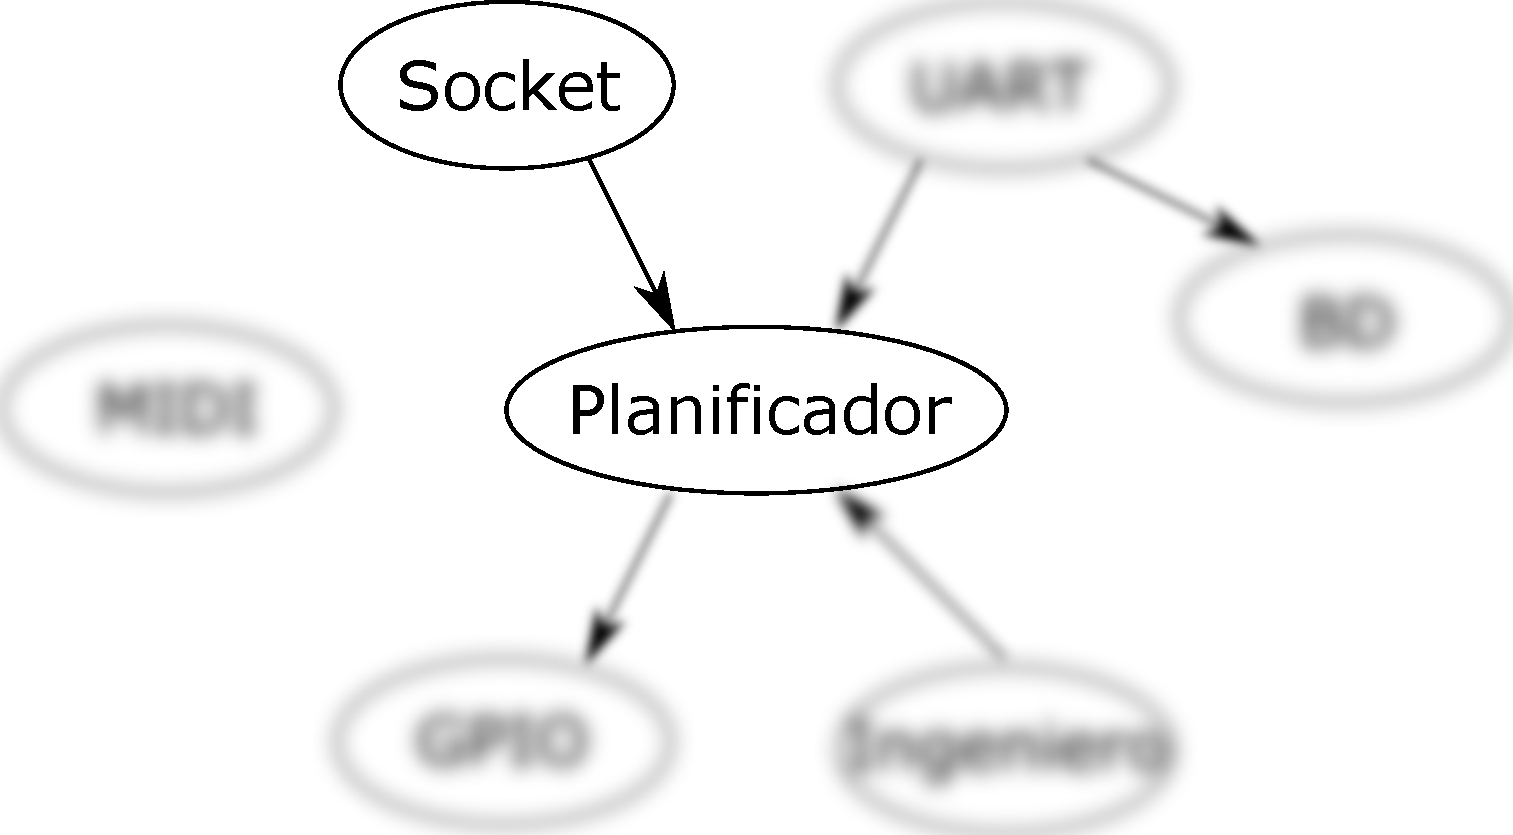
\includegraphics[width=\linewidth/2]{capitulo4/daemon_socket}
		\par\end{centering}
	\smallskip
	\caption{\label{fig:daemon_socket} Diagrama de uso del servidor socket.}
\end{figure} 

\smallskip

\subsection{Control del mando}
\label{subsec:daemon_mando}

Como hemos indicado en el capítulo anterior, el receptor del mando a distancia está conectado al \textit{Raspberry Pi} a través de los pines correspondientes al dispositivo \acrshort{UART} ---\textit{\acrlong{UART}}---, que controla los puertos serie. \cite{wiki_uart}

Este módulo tiene una topología análoga al control por \textit{socket}, tan solo cambia el origen y la forma de entrada de los datos. Establecerá una comunicación con el puerto serie e iniciará un bucle de escucha. La sintaxis del mensaje, como ya sabemos, es:

\begin{center}
	<Nº serie (7 \textit{bytes})> <Botón (1 \textit{byte})> <CRLF>
\end{center}

De esta forma, el servicio tan solo debe verificar el nº de serie y ejecutar la orden correspondiente.

Además de reconocer la pulsación del mando, es necesario consultar en la base de datos, que detallaremos en la sección \ref{sec:database}, la lista que corresponde al botón pulsado y los archivos contenidos, que serán transmitidos al planificador.

\subsubsection{Funciones}

Las funciones correspondientes a este módulo son las siguientes:

\begin{description}[style=nextline]
	\item[uart\_init () : \textit{integer}]
	Establece comunicación con el puerto serie.
	
	Devuelve 0 en caso de éxito y -1 en caso de error.
	
	\item[uart\_destroy ()]
	Cierra la comunicación.
	
	\item[uart\_loop ()]
	Despliega una hebra con un bucle de escucha y ejecuta las órdenes.
	
\end{description}

\subsubsection{Diagrama de uso}

Este bloque interacciona con el planificador en unos términos similares al \textit{socket}, y utiliza la interfaz de la base de datos.

\smallskip

\begin{figure}[H]
	\noindent \begin{centering}
		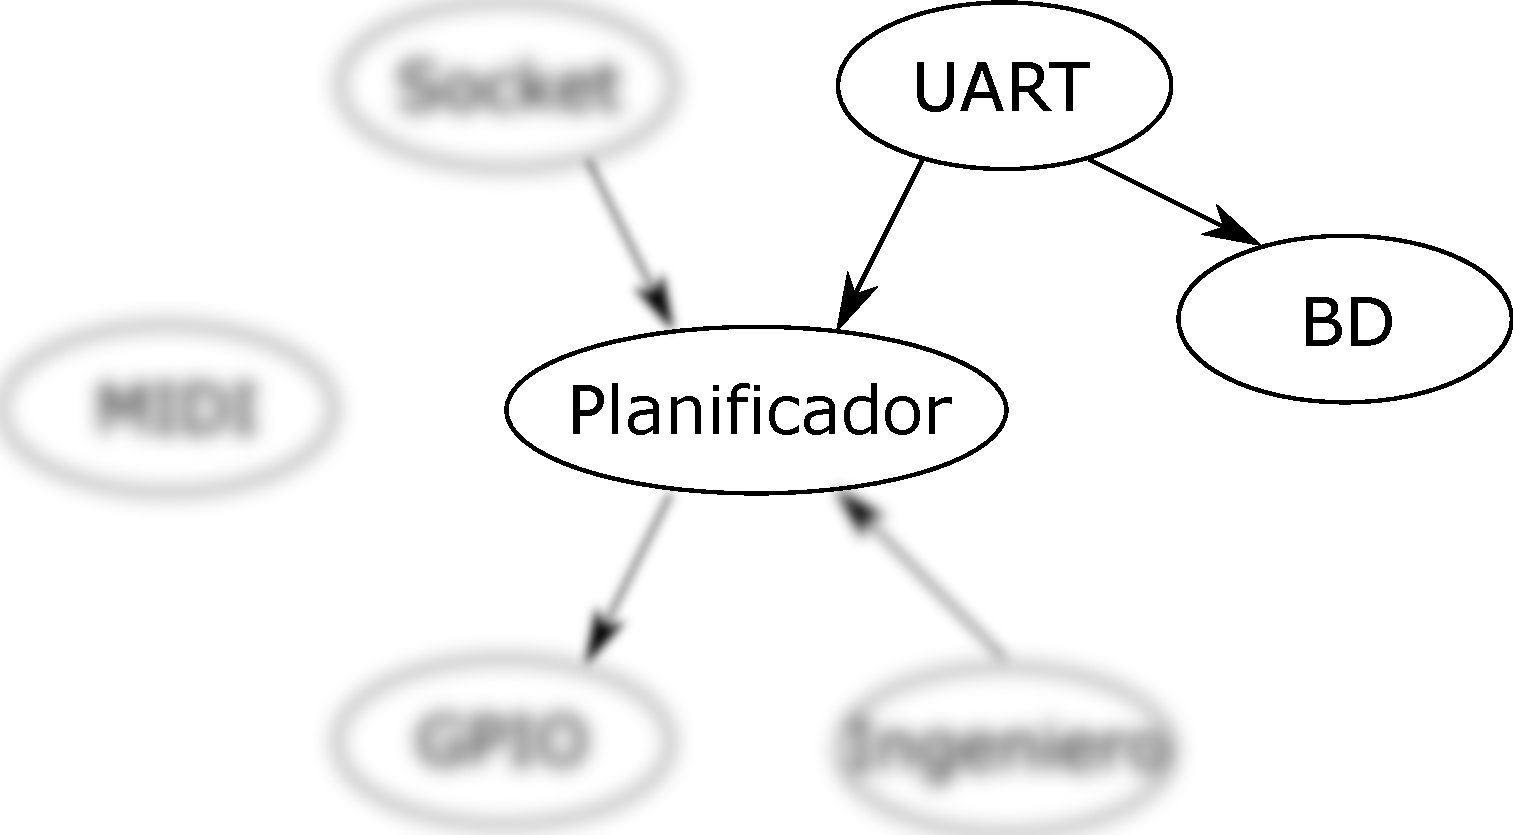
\includegraphics[width=\linewidth/2]{capitulo4/daemon_uart}
		\par\end{centering}
	\smallskip
	\caption{\label{fig:daemon_uart} Diagrama de uso del receptor de radio.}
\end{figure} 

\smallskip

\subsection{Comunicación con la base de datos}

La información relativa a la lista de reproducción asignada a un botón, así como la lista de partituras correspondientes, residirán en una base de datos, que definiremos en la sección \ref{sec:database}. Así, enmarcaremos un nuevo módulo dedicado a consultar la información requerida, ofreciendo una interfaz independiente del sistema de gestión de bases de datos que utilicemos, y de la propia base de datos.

\subsubsection{Funciones}

El sistema se comunicará con la base de datos mediante las siguientes funciones:

\begin{description}[style=nextline]
	\item[db\_init () : \textit{integer}]
	Inicia la comunicación con el gestor de bases de datos. Devuelve 0 en caso de éxito y -1 en caso de error.
	
	\item[db\_destroy ()]
	Cierra la comunicación.
	
	\item[db\_query (scores, idshortcut) : \textit{integer}]
	Realiza la consulta mencionada, asignando a \textit{scores} la lista de piezas a reproducir.
	
	\begin{description}
		\item[scores : \textit{array(string)}] Lista de rutas a las piezas.
		\item[idshortcut : \textit{integer}] ID del botón que se ha pulsado en el mando.
	\end{description}
	
	Devuelve el número de piezas asignadas (pudiendo ser 0), o -1 en caso de error.
	
\end{description}

\subsubsection{Diagrama de uso}

La interfaz de la base de datos es utilizada exclusivamente por el servidor del receptor de radio, sin perjuicio de que en un futuro podamos extender su funcionalidad, por lo que la hemos separado lógicamente del módulo \acrshort{UART}. El diagrama de uso es el siguiente:

\smallskip

\begin{figure}[H]
	\noindent \begin{centering}
		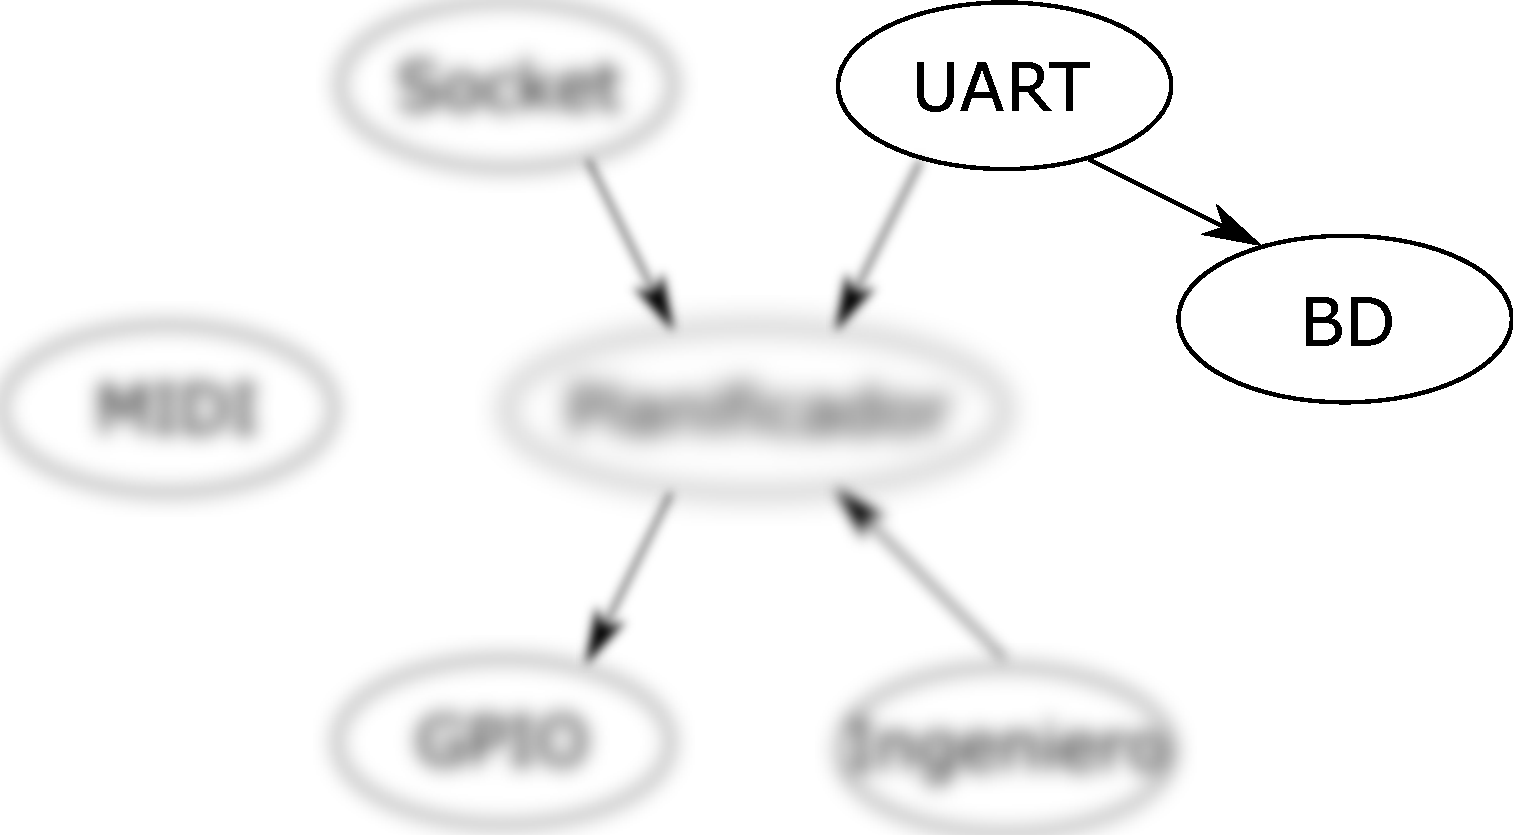
\includegraphics[width=\linewidth/2]{capitulo4/daemon_bd}
		\par\end{centering}
	\smallskip
	\caption{\label{fig:daemon_bd} Diagrama de uso de la interfaz de base de datos.}
\end{figure} 

\smallskip

\subsection{Planificador}
\label{subsec:planificador}

El planificador es la pieza principal del reproductor. Recibe las órdenes de los controladores y la lista de partituras a ejecutar. Una a una las lee con ayuda del módulo \acrshort{MIDI} y planifica los eventos de todas las pistas para lanzarlos a la salida en el momento necesario.

Al igual que otros módulos, utiliza una hebra para reproducir los archivos, pero en este caso es una hebra dinámica, que podrá ser iniciada, pausada y detenida por el resto de procesos, por lo que hay que tener en cuenta los problemas de concurrencia para garantizar la consistencia del sistema.

\subsubsection{Funciones}

La interfaz que el planificador ofrece es la que sigue:

\begin{description}[style=nextline]
	\item[player\_start (playlist, n, loop) : \textit{integer}]
	Inicia la reproducción de una lista de archivos. Si ya estaba reproduciendo una lista, primero detiene la reproducción y elimina la lista antigua.
	
	\begin{description}
		\item[playlist : \textit{array(string)}] Lista de rutas absolutas a los archivos que queremos reproducir.
		\item[n : \textit{integer}] Número de piezas que se han transmitido en el parámetro anterior.
		\item[loop : \textit{bool}] Utilizar (1) o no (0) reproducción en bucle.
	\end{description}
	
	Devuelve 0 en caso de éxito o -1 en caso de error.
	
	\item[player\_pause () : \textit{integer}]
	Pausa la reproducción, si estaba activa. Devuelve 0 en caso de éxito o -1 en caso de error.
	
	\item[player\_resume () : \textit{integer}]
	Reanuda la reproducción, si estaba pausada. Devuelve 0 en caso de éxito o -1 en caso de error.
	
	\item[player\_stop () : \textit{integer}]
	Detiene completamente la reproducción, si estaba activa o pausada. Si estaba parado, no hace nada. Devuelve 0 en caso de éxito o -1 en caso de error.
	
	\item[player\_wait () : \textit{integer}]
	Espera a que el reproductor se detenga. Solo tiene sentido llamarla en caso de no estar reproduciendo en bucle. Devuelve 0 en caso de éxito o -1 en caso de error.
	
	\item[player\_state (file) : \textit{enum}]
	Indica el estado actual del planificador. Tales estados se detallan en el apartado siguiente.
	
	\begin{description}
		\item[file : \textit{string}] Es un parámetro de salida, sobre él se escribe el nombre del archivo que se estaba reproduciendo. Solo es válido si el reproductor está activo o en pausa.
	\end{description}
	
	Devuelve el estado actual del reproductor, a saber entre los estados contemplados en la máquina.
	
	\item[player\_engineer\_enter () : \textit{integer}]
	Detiene el reproductor, bloquea el planificador y entra en modo Ingeniería. Devuelve 0 en caso de éxito o -1 en caso de error, como estar ya dentro del modo Ingeniería.
	
	\item[player\_engineer\_exit () : \textit{integer}]
	Sale del modo Ingeniería y debloquea el planificador. Devuelve 0 en caso de éxito o -1 en caso de error, como no estar dentro del modo Ingeniería.
	
\end{description}

\subsubsection{Máquina de estados}

Para gestionar su funcionamiento, el planificador utiliza una pequeña cantidad de estados, que mostramos a continuación:

\smallskip

\begin{figure}[H]
	\noindent \begin{centering}
		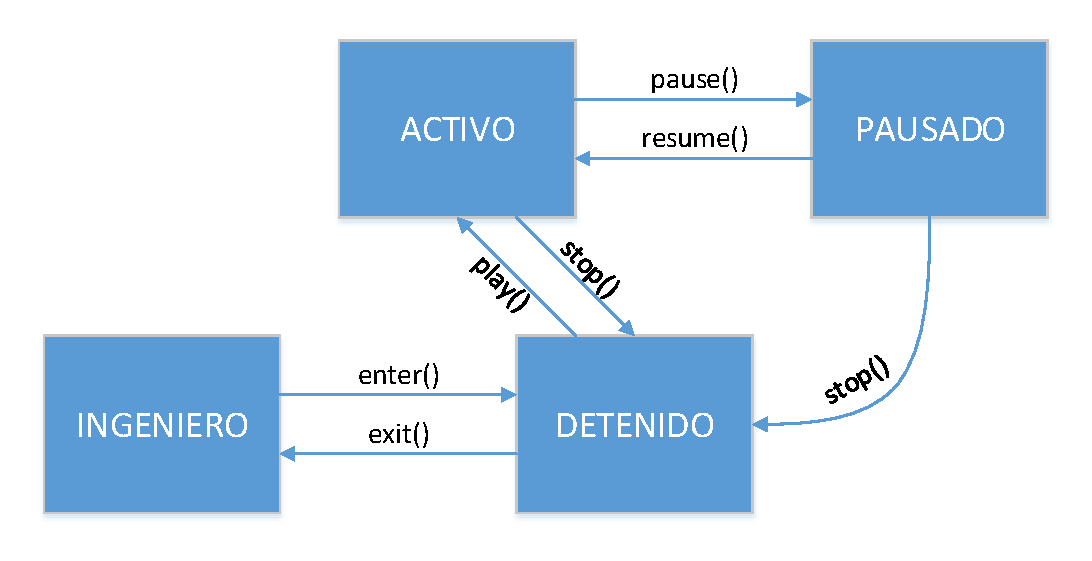
\includegraphics[width=\linewidth/2]{capitulo4/sched}
		\par\end{centering}
	\smallskip
	\caption{\label{fig:sched} Diagrama de estados del planificador.}
\end{figure} 

\smallskip

\begin{description}
	\item[Activo] En funcionamiento, reproduciendo activamente una partitura.
	\item[Pausado] No reproduce, mantiene el estado del órgano en el módulo de salida.
	\item[Parado] En espera. Es el estado inicial.
	\item[Ingeniero] Bloqueado, en modo Ingeniería. Ha cedido el control del módulo de salida.
\end{description}

\subsubsection{Algoritmo básico}

Para que todas las pistas se ejecuten simultáneamente, el planificador recorre en cada ciclo todas las listas, avanzando mientras sea el momento de ejecutar el evento correspondiente ($\Delta=0$). Cuando se ha llegado a un evento con $\Delta > 0$ en todas las pistas, se busca el menor de ellos y se resta al \textit{delta} de todos los eventos. A continuación, se solicita al sistema operativo la espera correspondiente al tiempo restado, y se repite el ciclo. El algoritmo termina cuando todas las pistas han llegado al final.

\smallskip

\begin{algorithmic}
	\LOOP
		\STATE $mindelta \gets \infty$
		\STATE $i\gets 0$
		\WHILE {$i < n_{tracks}$}
			\WHILE {$event_i.delta = 0$ \AND \NOT ($event_i.type = METAEVENT$ \AND \\ $event_i.metaevent.type = END\_OF\_TRACK$)}
				\IF {$event_i.type = NOTE\_ON$}
					\STATE $output\_noteon(i, event_i.param1)$
				\ELSE 
					\IF {$event_i.type = NOTE\_OFF$}
						\STATE $output\_noteoff (i, event_i.param1)$
					\ENDIF
				\ENDIF
				\STATE $event_i \gets event_i.next$
			\ENDWHILE
			\IF {$event_i.delta > 0$ \AND $event_i.delta < mindelta$}
				\STATE $mindelta \gets event_i.delta$
			\ENDIF
		\ENDWHILE
		\STATE $i \gets 0$
		
		\WHILE {$i < n_{tracks}$}
			\STATE $event_i.delta \gets event_i.delta - min$
		\ENDWHILE
		\STATE $sleep (mindelta)$
	\ENDLOOP
\end{algorithmic}

\smallskip

\subsubsection{Diagrama de uso}

Como parte central del programa, y al contrario que el resto de componentes, el planificador está conectado con la mayoría de módulos, actuando como mediador y coordinador entre aquellos que reciben órdenes y los que facilitan la salida de información.

\smallskip

\begin{figure}[H]
	\noindent \begin{centering}
		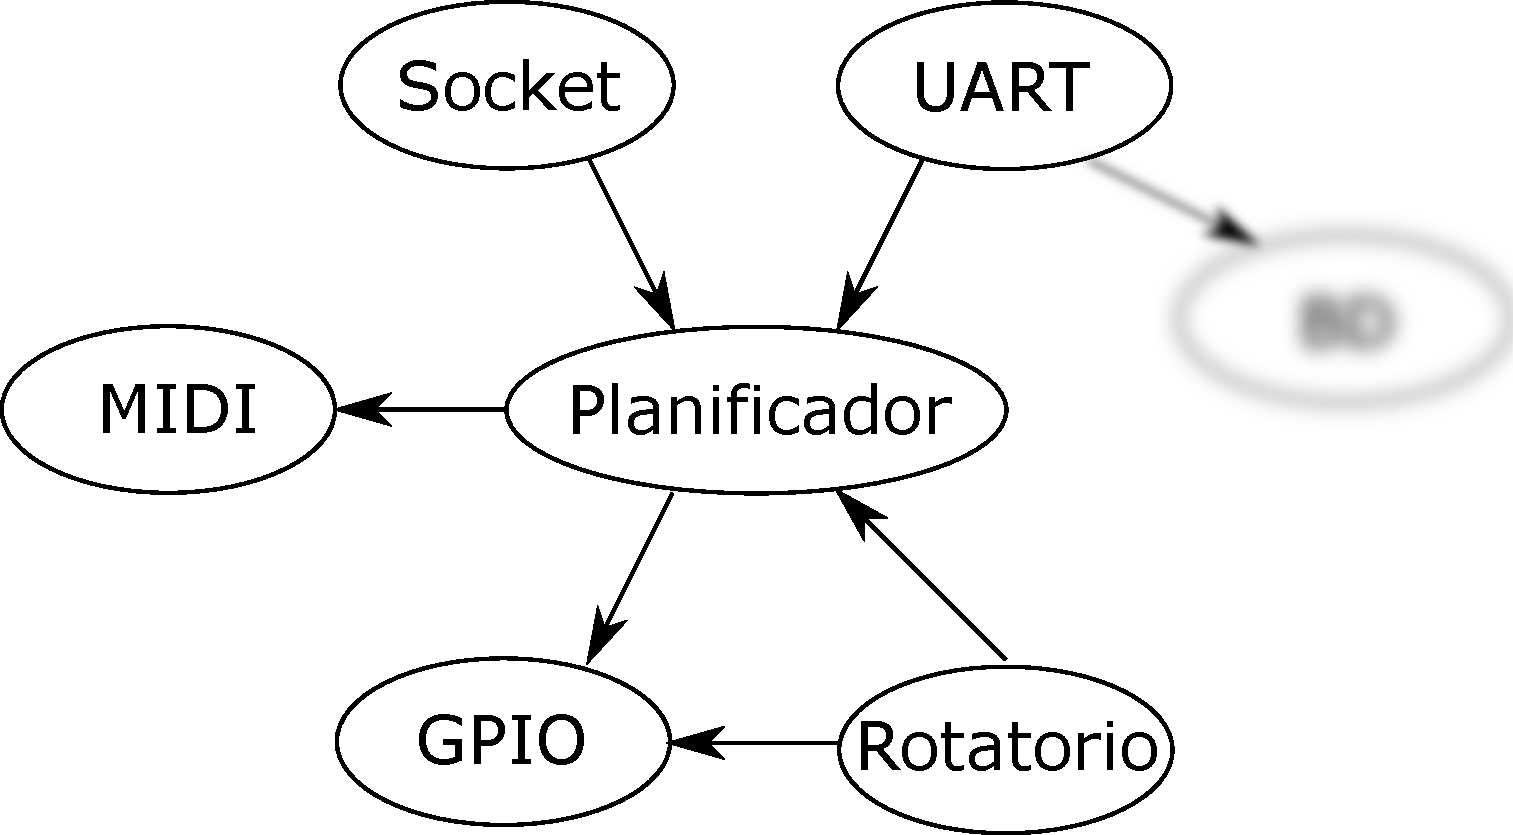
\includegraphics[width=\linewidth/2]{capitulo4/daemon_scheduler}
		\par\end{centering}
	\smallskip
	\caption{\label{fig:daemon_scheduler} Diagrama de uso del planificador.}
\end{figure} 

\smallskip

\begin{itemize}
	\item Los servidores de \textit{socket} y de \acrshort{UART}, y el control de interfaz reducida, envían las órdenes de control.
	\item El módulo \acrshort{MIDI} es utilizado para descodificar los archivos de entrada.
	\item La información extraída se dirige al módulo de salida (\acrshort{GPIO}) para llegar a la \acrshort{PCB}.
\end{itemize}

\subsection{Modo Ingeniería}

El sistema requiere un modo de mantenimiento para regular la mecánica, al que se accederá localmente, a través de una interfaz reducida que controlaremos con el codificador rotatorio y el \acrshort{LCD}.

El codificador permitirá acceder al modo Ingeniería, que detendrá la reproducción ---si estaba en funcionamiento--- y  aislará el planificador, ganando acceso directo a la salida \acrshort{GPIO}.

Vamos a diseñar la interfaz como una máquina de estados: Inicialmente el modo Ingeniería está desactivado, girando el botón se nos dará la opción de activarlo, y al pulsarlo entraremos en él. Se activará la nota más baja de la primera pista, al girar el botón podremos movernos cíclicamente por todas las notas de esa pista. Pulsando el botón cambiamos a la segunda pista, luego a la tercera, y así hasta la última. Si apretamos nuevamente el botón, volvemos al menú que nos permitirá salir del modo Ingeniería.

Este diagrama muestra las transiciones entre los estados:

\smallskip

\begin{figure}[H]
	\noindent \begin{centering}
		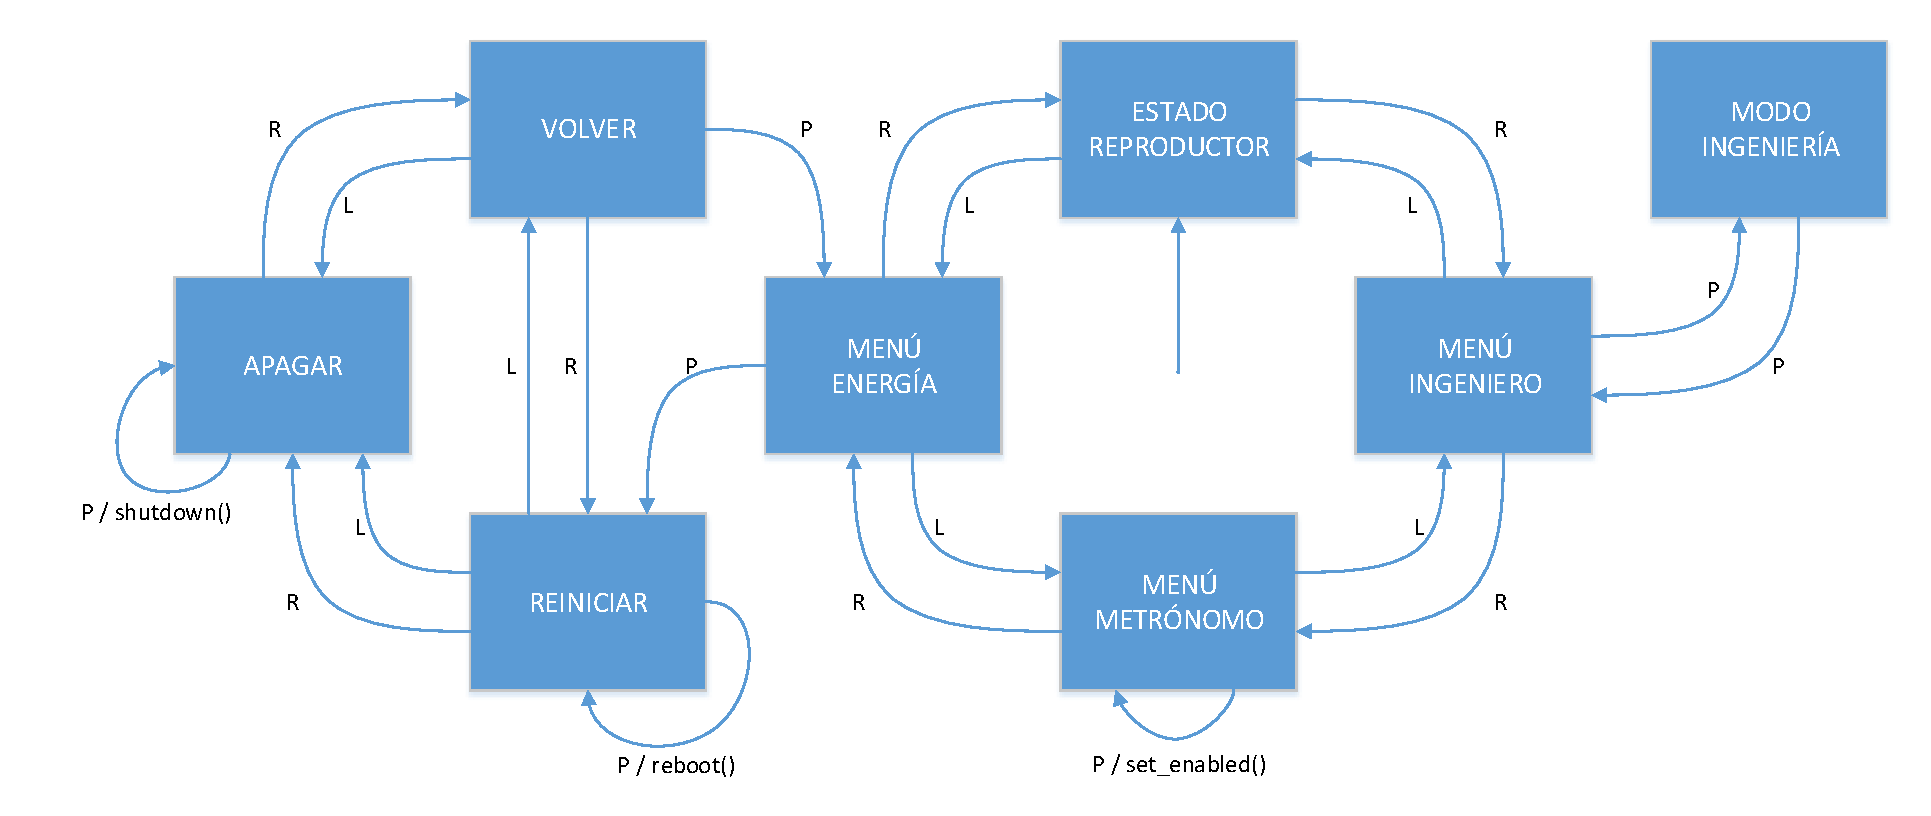
\includegraphics[width=\linewidth*3/4]{capitulo4/engineer}
		\par\end{centering}
	\smallskip
	\caption{\label{fig:engineer} Máquina de estados de la interfaz reducida.}
\end{figure} 

\smallskip

\begin{description}
	\item[OFF] Estado inicial, modo Ingeniería apagado. Mostrará el estado del reproductor.
	\item[MENU] Ofrece la opción de entrar en el modo Ingeniería.
	\item[ON] Modo Ingeniería activado, los subestados dependen de la pista y la nota actuales
\end{description}

\subsubsection{Diagrama de uso}

El módulo que controla el modo Ingeniería interacciona con el planificador, para detenerlo y aislarlo del \acrshort{GPIO}, y con el módulo de salida, que maneja el propio \acrshort{GPIO}, para manipular el estado.

\smallskip

\begin{figure}[H]
	\noindent \begin{centering}
		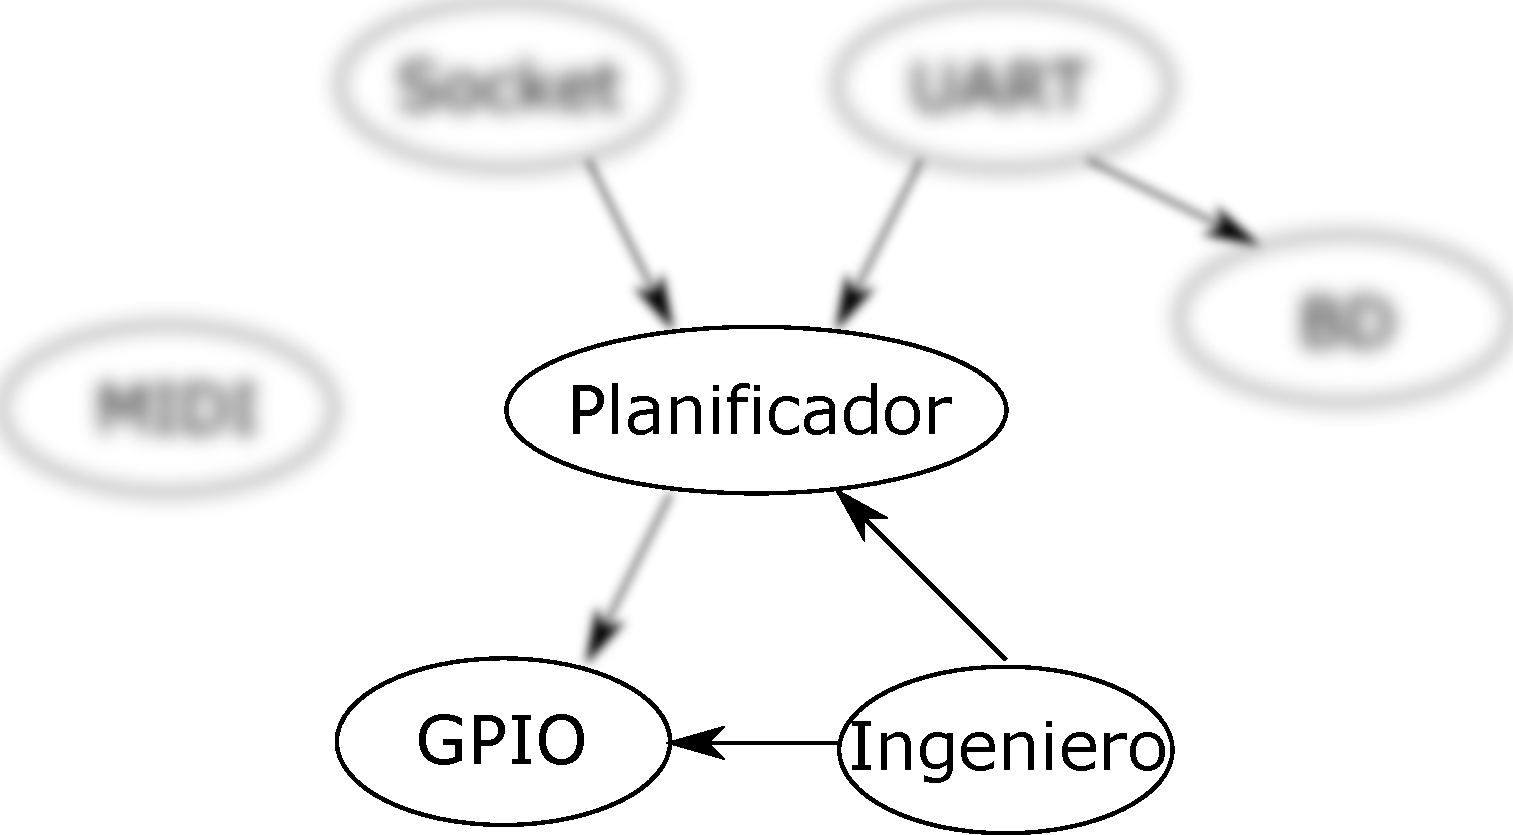
\includegraphics[width=\linewidth/2]{capitulo4/daemon_engineer}
		\par\end{centering}
	\smallskip
	\caption{\label{fig:daemon_engineer} Diagrama de uso del modo Ingeniería.}
\end{figure} 

\smallskip

\subsection{Salida hacia la PCB}
\label{subsec:output}

El reproductor delega en el módulo de salida las siguientes funciones:

\begin{enumerate}
	\item Dirigir las pistas de \acrshort{MIDI} al canal de salida correspondiente.
	\item Almacenar el estado de salida (notas pulsadas y no pulsadas).
	\item Volcar la información en el \acrshort{GPIO}.
\end{enumerate}

Éste será el único módulo que tendremos que cambiar a la hora de pasar de un órgano a otro. El hecho de aislar la salida también nos da flexibilidad para sustituir la interfaz \acrshort{GPIO} por otro tipo de salida, como la consola, con fines de mantenimiento y depuración.

\subsubsection{Funciones}

Las siguientes funciones conforman la interfaz del módulo:

\begin{description}[style=nextline]
	\item[output\_init () : \textit{integer}]
	Inicializa los componentes de la salida. Devuelve 0 en caso de éxito o -1 en caso de error.
	
	\item[output\_destroy ()]
	Cierra el módulo de salida y libera la memoria ocupada.
	
	\item[output\_noteon (track, note)]
	Marcar una nota para activar en el sistema.
	
	\begin{description}
		\item[track : \textit{integer}] Índice de la pista \acrshort{MIDI}.
		\item[note : \textit{integer}] Número de nota \acrshort{MIDI}.
	\end{description}
	
	\item[output\_noteon (track, note)]
	Marcar una nota para apagarla en el sistema.
	
	\begin{description}
		\item[track : \textit{integer}] Índice de la pista \acrshort{MIDI}.
		\item[note : \textit{integer}] Número de nota \acrshort{MIDI}.
	\end{description}
	
	\item[output\_update ()]
	Vuelca el estado en la salida.
	
	\item[output\_panic ()]
	Vuelve al estado inicial (silenciar todas las notas), y lo vuelca en la salida.
	
	\item[output\_silence ()]
	Silencia todas las notas en la salida, pero mantiene el estado. Útil para pausar la reproducción.
	
\end{description}

\subsubsection{Mapeo de pistas y canales}

Nuestra especificación deja abierta la estructura que pueda tener un archivo \acrshort{MIDI}. A pesar de que el sistema podrá descodificar \acrshort{MIDI} estándar, para lograr una óptima ejecución, la pieza deberá adaptarse a cada órgano concreto.

El módulo de salida permitirá asignar cada pista \acrshort{MIDI}, que normalmente corresponde a un pentagrama de la partitura, a un canal de salida diferente. La asignación por defecto, para el órgano estudiado, será la siguiente:

\smallskip

\begin{figure}[H]
	\noindent \begin{centering}
		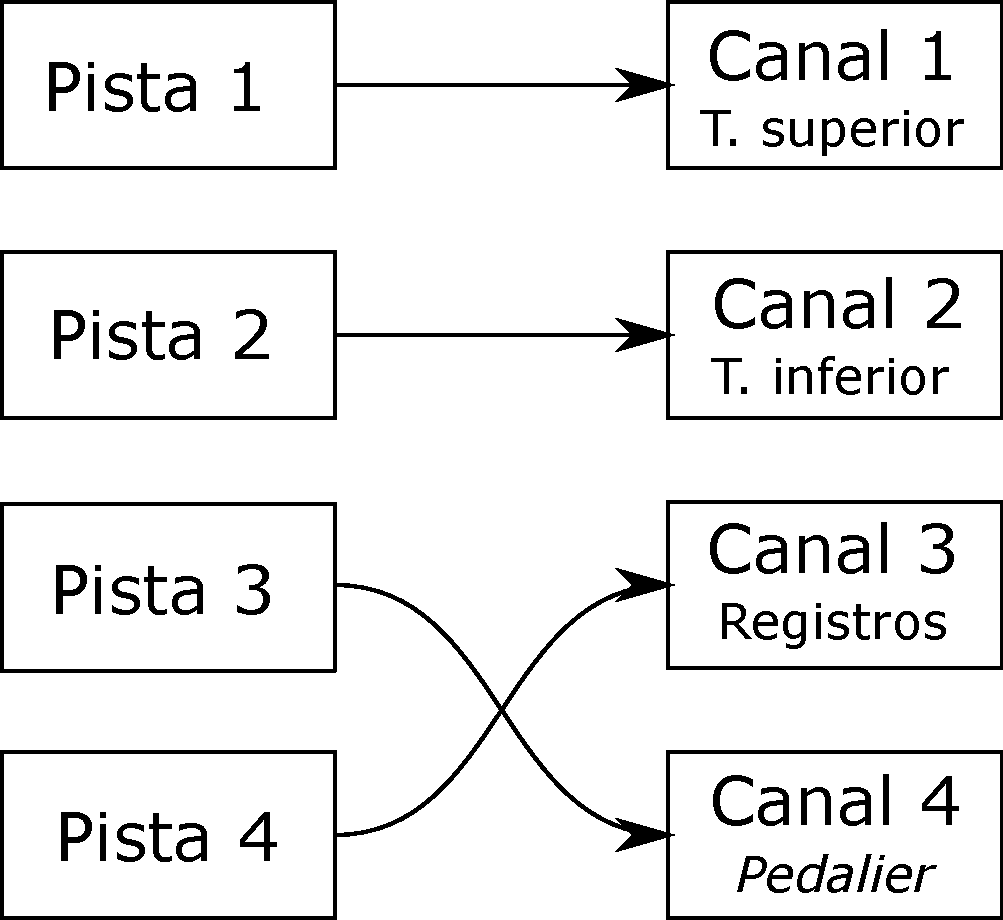
\includegraphics[width=\linewidth/3]{capitulo4/map}
		\par\end{centering}
	\smallskip
	\caption{\label{fig:map} Asignación de pistas MIDI y canales de salida.}
\end{figure} 

\smallskip

\subsubsection{Diagrama de uso}

La interfaz de salida es utilizada principalmente por el planificador y, solo cuando éste entra en modo Ingeniería, es accedida por el módulo del mismo nombre, para poner a prueba la mecánica del sistema.

\smallskip

\begin{figure}[H]
	\noindent \begin{centering}
		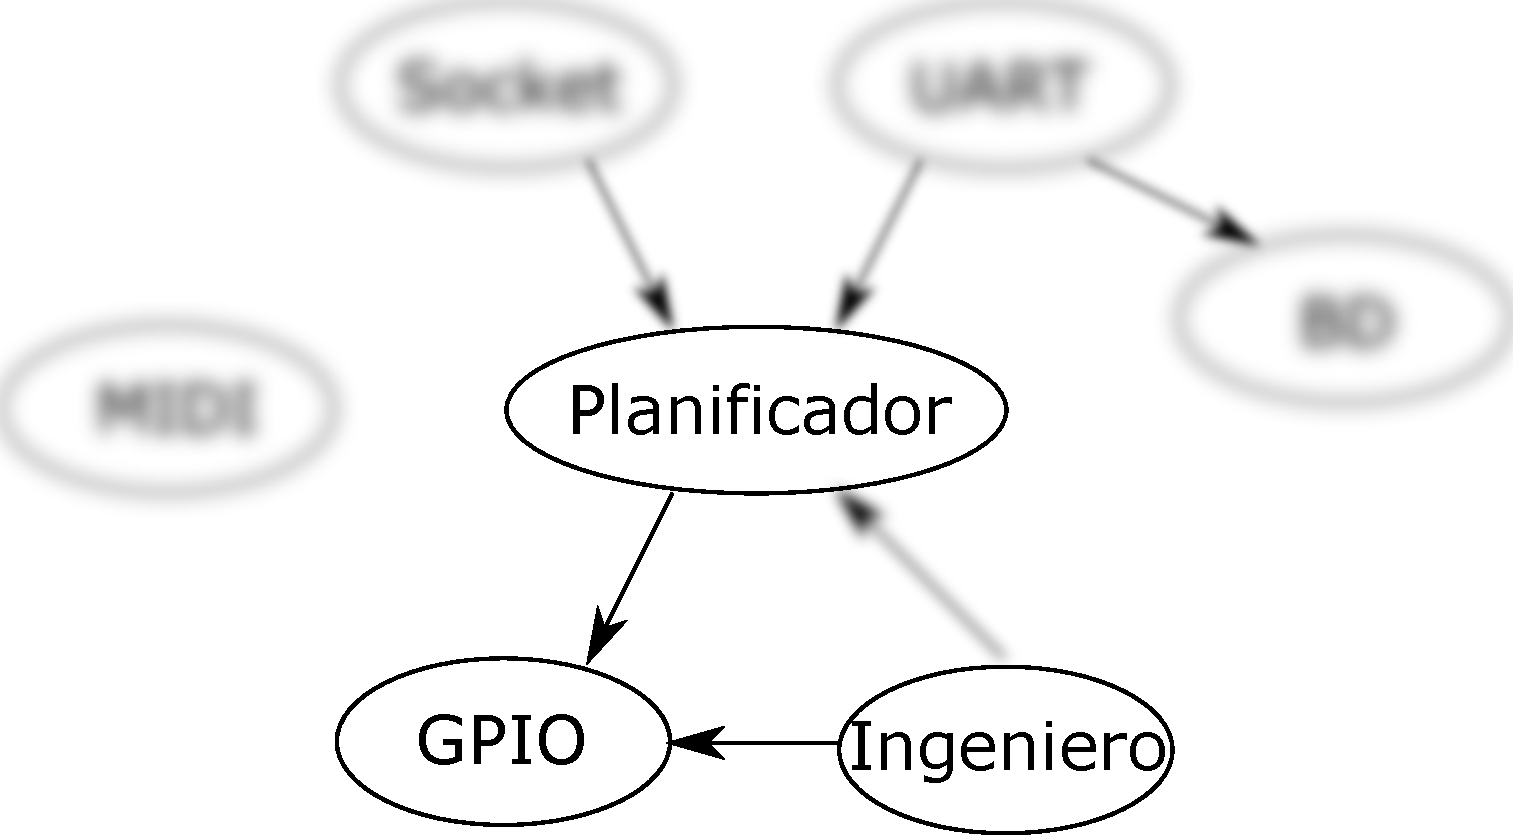
\includegraphics[width=\linewidth/2]{capitulo4/daemon_gpio}
		\par\end{centering}
	\smallskip
	\caption{\label{fig:daemon_gpio} Diagrama de uso del módulo de salida.}
\end{figure} 

\smallskip

\subsection{Seguridad}

A pesar de que el acceso al sistema se hará siempre con autentificación de usuario, nos interesa controlar que no todos los usuarios, o no todas las aplicaciones, se conecten al \textit{socket}. La seguridad de Linux recae en gran parte sobre su sistema de archivos y permisos. Se creará un nombre de usuario de sistema para ser utilizado exclusivamente por el \textit{socket}, que tendrá permisos de lectura y escritura para dicho usuario y su grupo.

Para autorizar a un usuario a acceder al \textit{socket}, simplemente hay que añadirlo al grupo del usuario propietario.

Por otro lado, el demonio se ejecuta con permisos de \textit{superusuario}, y es inseguro mantenerse durante toda la ejecución con tales privilegios. A pesar de que introduciremos medidas de seguridad en los clientes que desarrollemos para el sistema, reduciremos los permisos después de inicializar el proceso, como medida adicional para evitar problemas.

\section{Base de datos}
\label{sec:database}

La información que queremos almacenar funciona de la siguiente forma:

\begin{enumerate}
	\item Las partituras se guardan en un archivo, cuyo nombre no tiene que coincidir con el título de la partitura.
	\item De una partitura podremos conocer su duración.
	\item Una lista de reproducción es una colección de partituras, y le asignaremos un nombre.
	\item Cada partitura pertenecerá a una lista de reproducción, y solo a una.
	\item Un botón se distingue por su código, y se le asigna a una lista de reproducción, sin perjuicio de que una lista esté asignada a varios botones. Naturalmente, puede haber listas que no estén asignadas a ningún botón.
\end{enumerate}

\subsection{Modelo entidad-relación}

Atendiendo a los requisitos propuestos, modelamos nuestros datos según el siguiente diagrama:

\smallskip

\begin{figure}[H]
	\noindent \begin{centering}
		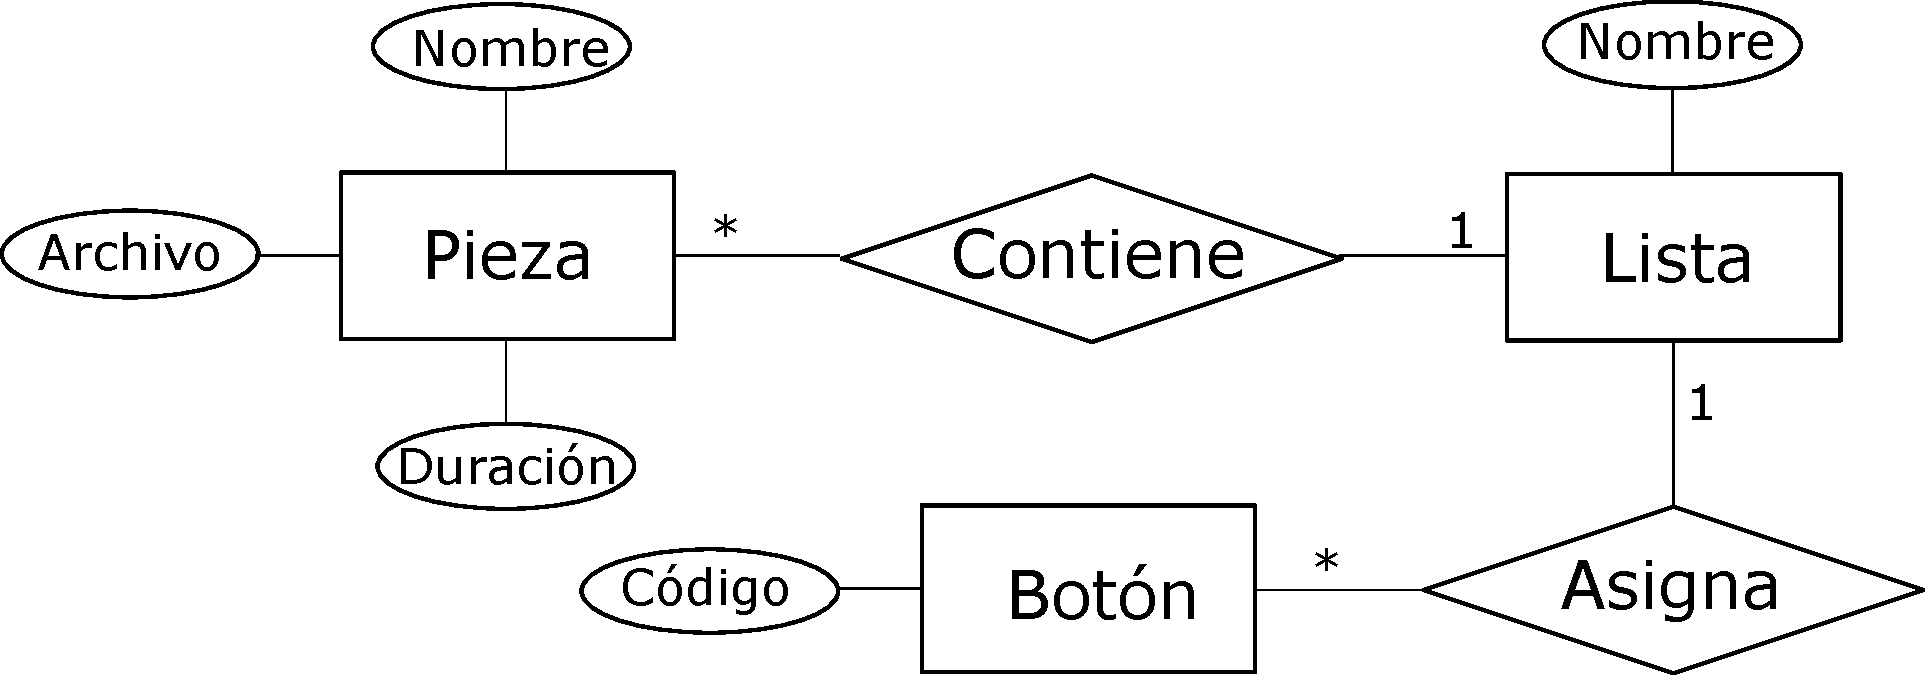
\includegraphics[width=\linewidth*3/4]{capitulo4/bd_er}
		\par\end{centering}
	\smallskip
	\caption{\label{fig:bd_er} Modelo entidad-relación.}
\end{figure} 

\smallskip

\subsection{Modelo relacional}

Una vez hemos considerado las entidades, sus atributos y las relaciones, diseñamos el modelo de datos, que depende del tipo de sistema de gestión de bases de datos ---\acrshort{DBMS} (\textit{\acrlong{DBMS}})--- que vayamos a utilizar. En nuestro caso, utilizaremos un \acrshort{DBMS} relacional \cite{bdrel}.

\begin{enumerate}
	\item Convertimos en relaciones (tablas) todas las entidades y las relaciones del modelo entidad-relación.
	\item Los atributos de las entidades pasan a ser atributos de las relaciones correspondientes.
	\item Buscamos llaves candidatas y escogemos una como llave primaria. En el caso de Pieza y Lista, no tenemos llave candidata, así que añadimos un ID a cada relación.
	\item Las relaciones Contiene y Asigna tienen cardinalidad N-1, de forma que comparten la clave primaria. Fusionamos Contiene en Pieza y Asigna en Botón.
\end{enumerate}

Una vez hecho esto, el modelo resultante es el siguiente:

\smallskip

\begin{figure}[H]
	\noindent \begin{centering}
		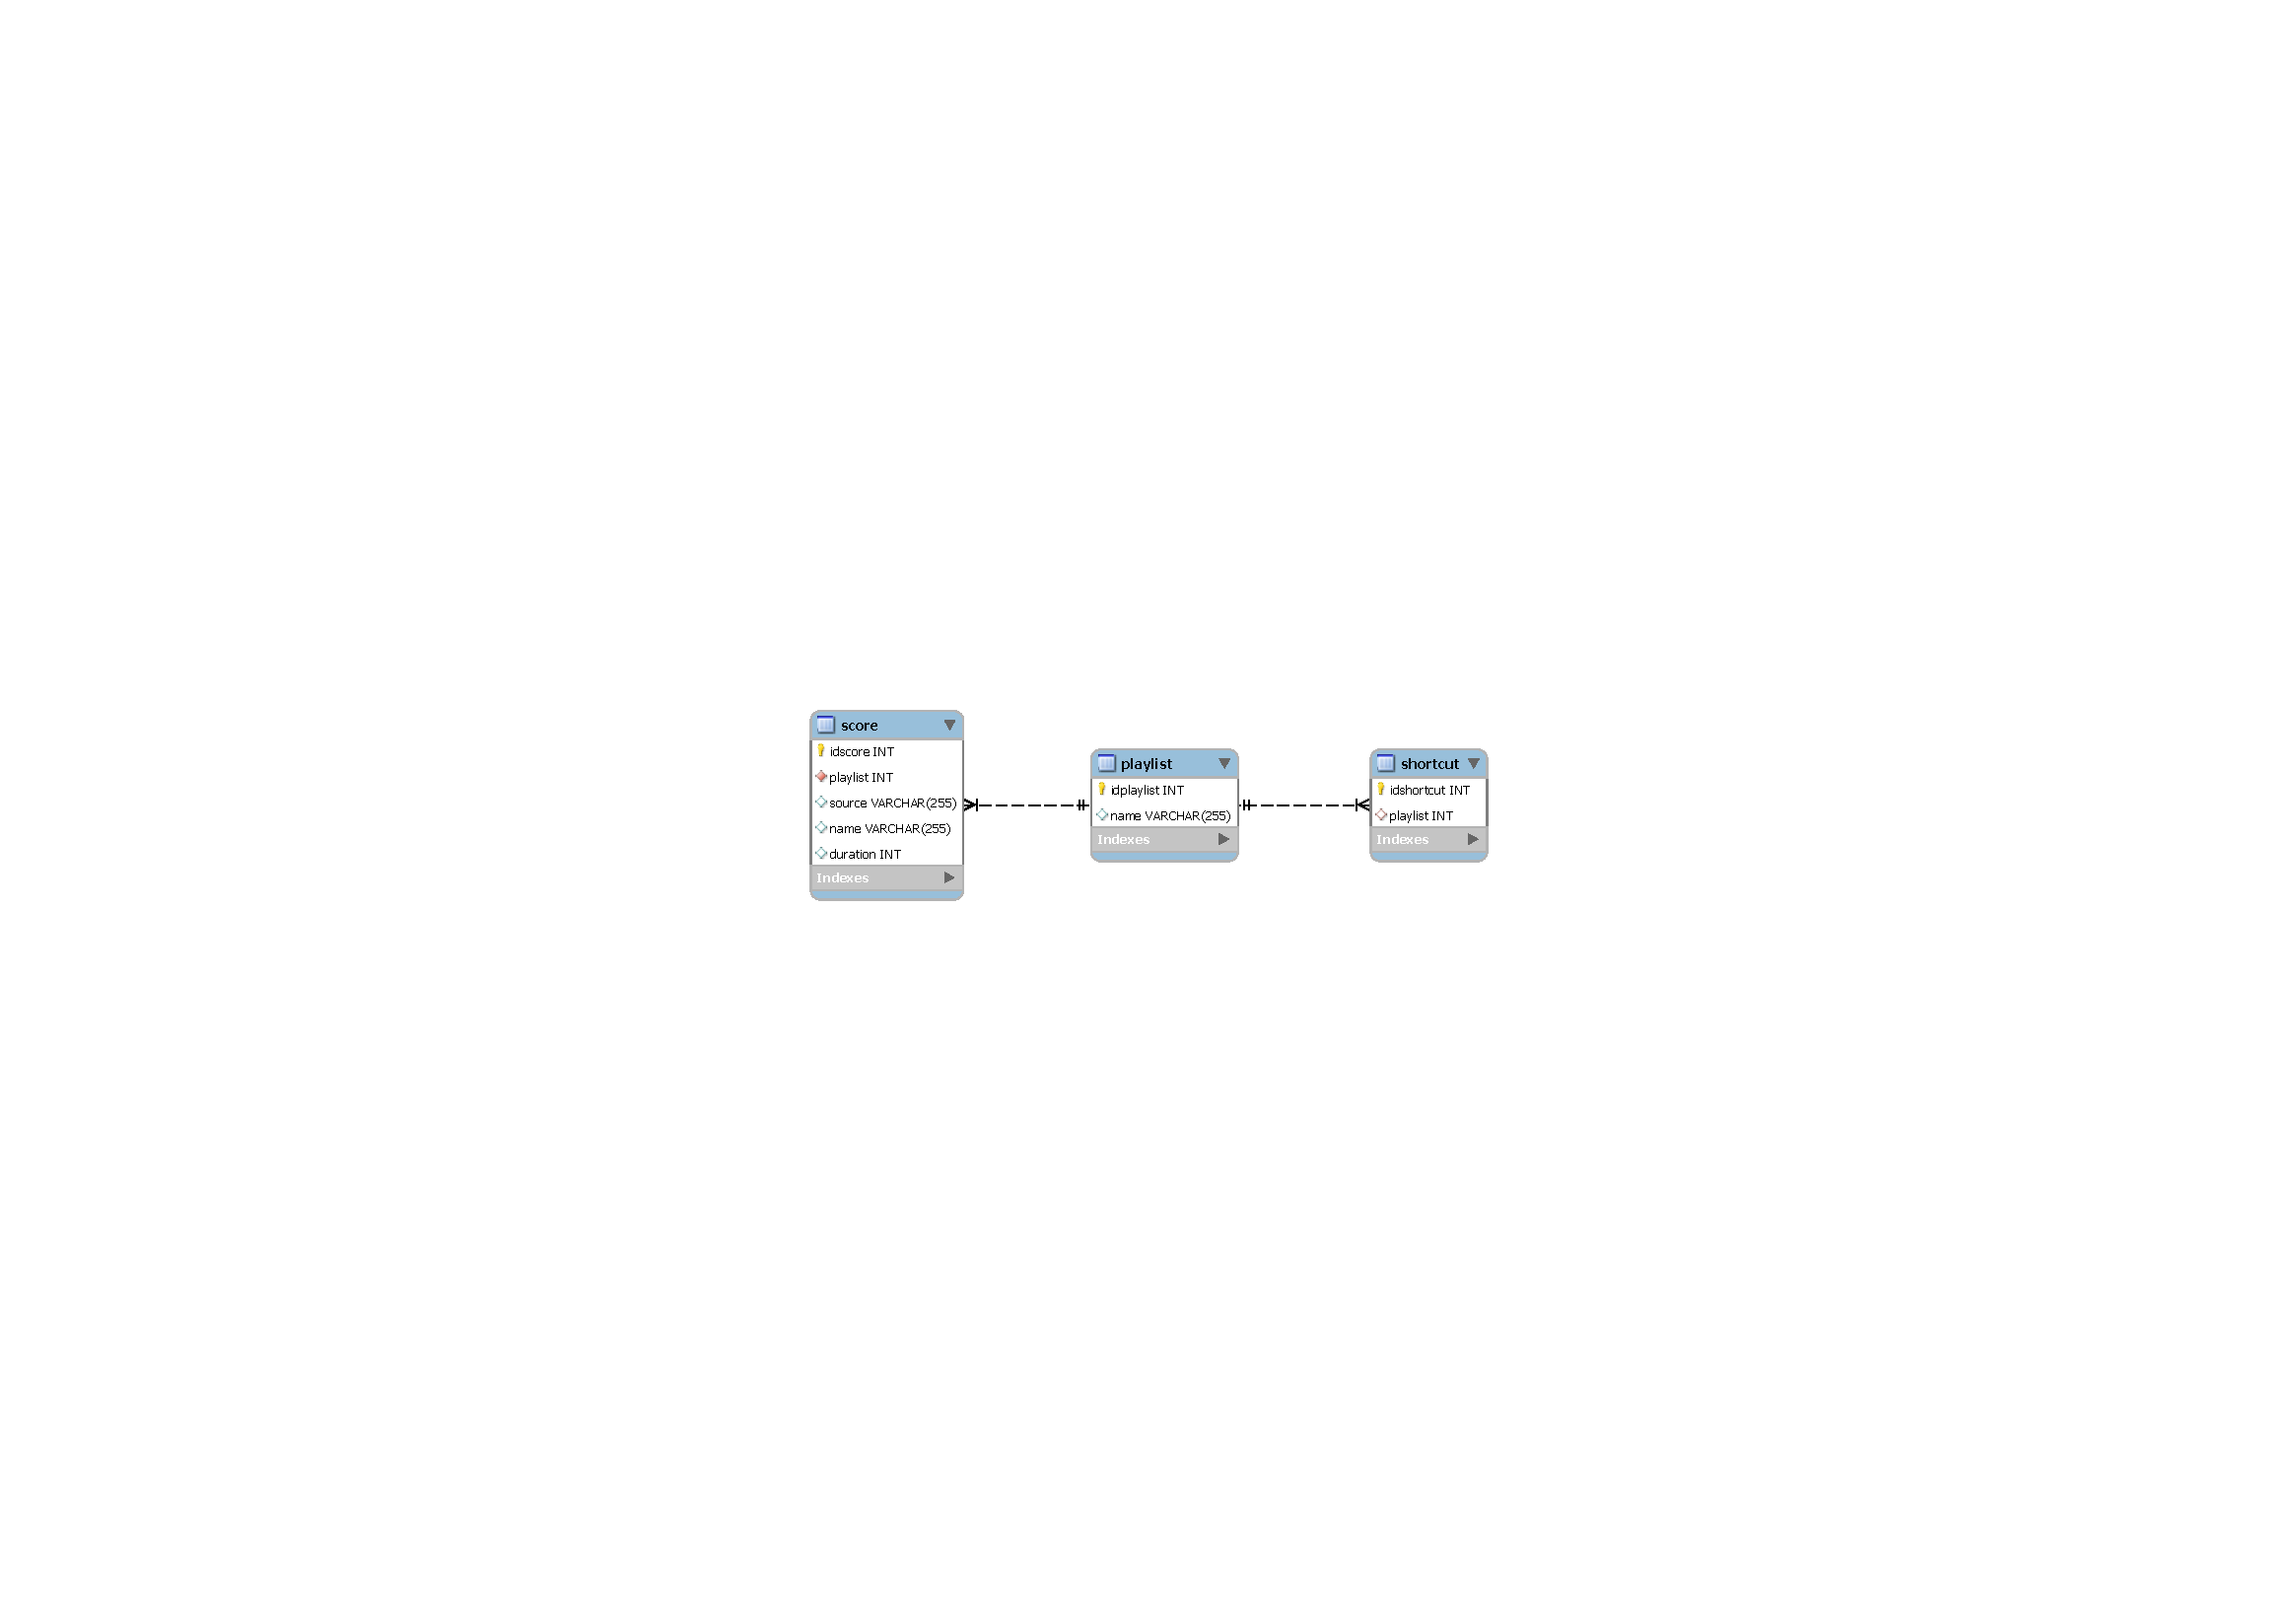
\includegraphics[clip=true, trim=390 340 390 340, width=\linewidth*3/4]{capitulo4/bd_rel}
		\par\end{centering}
	\smallskip
	\caption{\label{fig:bd_rel} Modelo relacional.}
\end{figure} 

\smallskip

\subsection{Consistencia}

Para garantizar que la base de datos mantendrá la información coherente y sin anomalías, estudiamos las relaciones para normalizarlas. Podemos verificar que nuestro modelo relacional está en 5ª forma normal, atendiendo a las siguientes condiciones:

\begin{description}
	\item[1FN] El \acrshort{SGBD} relacional se encarga de que se cumpla la forma normal más básica: las columnas son regulares, no habrá filas duplicadas (por la llave primaria) ni orden alguno entre filas o columnas. \cite{wiki_1fn}
	\item[2FN] Todos los atributos secundarios de cada tabla dependen de la llave primaria, por tanto, está en segunda forma normal. \cite{wiki_2fn}
	\item[3FN] No existen atributos secundarios que dependan transitivamente de la llave primaria, entonces, está en tercera forma normal. \cite{wiki_3fn}
	\item[FNBC] La forma normal de Boyce-Codd establece que los únicos determinantes sean las claves candidatas. Como el modelo está en 3FN y no existen llaves candidatas compuestas, podemos decir que está también en 3FN. \cite{wiki_fnbc}
	\item[4FN] La cuarta forma normal extiende la FNBC exigiendo que no existan dependencias multivaluadas no triviales. Este modelo no tiene dependencias multivaluadas, de forma que está en 4FN. \cite{wiki_4fn}
	\item[5FN] Por último, la quinta forma normal especifica que, además de todo lo anterior, cada dependencia de unión sea implicada por claves candidatas. Esto se cumple en nuestro modelo, ya que toda llave externa se vincula a la llave primaria de otra relación. \cite{wiki_5fn}
\end{description}

Nuestro modelo relacional cumple todas las exigencias de las formas normales tenidas en cuenta, con lo que podemos garantizar que el modelo es consistente.

\smallskip

\begin{figure}[H]
	\noindent \begin{centering}
		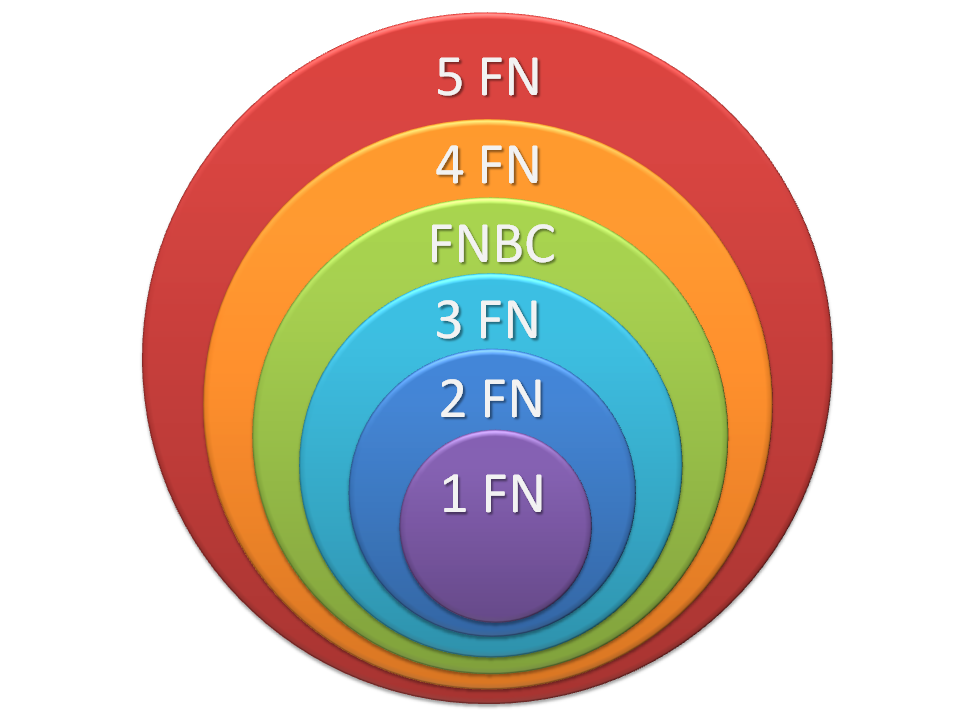
\includegraphics[width=\linewidth/2]{capitulo4/bd_fn}
		\par\end{centering}
	\smallskip
	\caption[Relación entre las formas normales.]{\label{fig:bd_fn} Relación entre las formas normales. \cite{wiki_normal}}
\end{figure} 

\smallskip

\section{Control remoto}

Hasta ahora hemos diseñado el \textit{back-end} del sistema, con todas las características que darán funcionalidad a nuestra solución. Pero aún no tenemos una interfaz que permita al usuario interactuar con el sistema, más que el control del mando a distancia o desde la \acrshort{PCB}.

El próximo paso es concebir el \textit{front-end} que, a tenor de los requisitos que propusimos al inicio, ofrezca al usuario la interfaz más completa posible. Frecuentemente la funcionalidad viene contrapuesta a la facilidad de uso; es nuestra tarea encontrar el mejor equilibrio posible.

Vamos a diseñar una solución enfocada al uso remoto con ayuda de un explorador de Internet, como \textit{Chrome}, \textit{Firefox} o \textit{Safari}, con lo que crearemos un servidor \textit{web}. El control del órgano queda pues estructurado de la siguiente forma:

\smallskip

\begin{figure}[H]
	\noindent \begin{centering}
		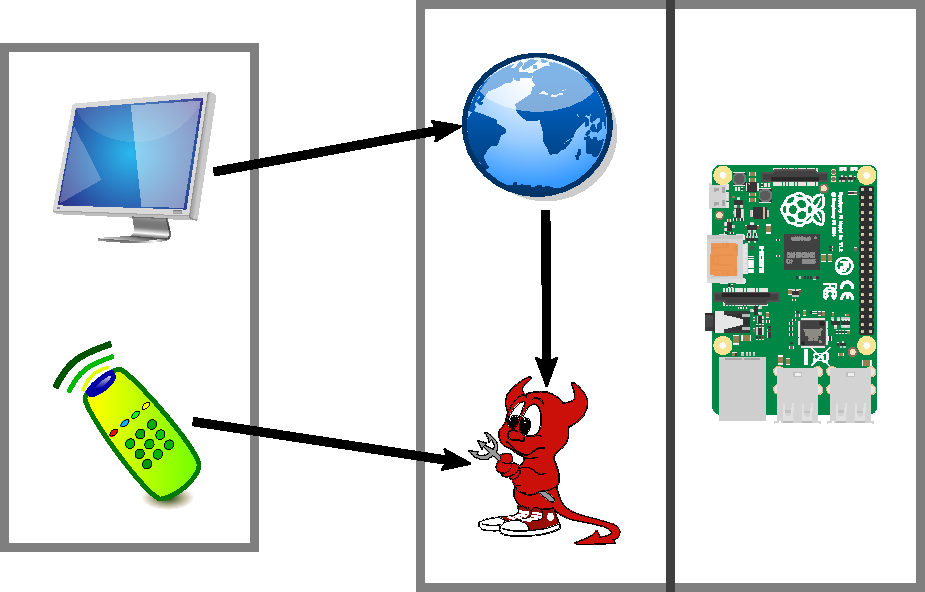
\includegraphics[width=\linewidth*2/3]{capitulo4/despliegue}
		\par\end{centering}
	\smallskip
	\caption[Comunicación entre el cliente y el software del sistema]{\label{fig:despliegue} Comunicación entre el cliente y el software del sistema. \cite{svg_raspberry}}
\end{figure} 

\smallskip

En primer lugar será especificar los casos de uso que nos enfrentarán al usuario. Después, concebiremos el aspecto de la interfaz y por último esbozaremos la estructura del diseño.

\subsection{Casos de uso}

A continuación enumeramos una relación de casos de uso que deberá cubrir la interfaz de usuario:

\begin{enumerate}
	\item Identificarse en el sistema como usuario autorizado.
	\item Salir del sistema, en el sentido de que al entrar de nuevo haya que identificarse.
	\item Controlar la reproducción directamente, a saber:
	
	\begin{enumerate}
		\item Ver el nombre de la pieza que se está reproduciendo.
		\item Ejecutar una lista de reproducción en bucle.
		\item Escoger una pieza de la lista para reproducirla.
		\item Pausar la reproducción de una pieza.
		\item Reanudar la ejecución de una pieza, si estaba pausada.
		\item Detener completamente la reproducción.
		\item Avanzar en la lista y reproducir la siguiente pieza.
		\item Retroceder en la lista y reproducir la partitura anterior.
	\end{enumerate}
	
	\item Gestionar listas de reproducción:
	
	\begin{enumerate}
		\item Crear una nueva lista, dándole un nombre.
		\item Visualizar todas las listas existentes.
		\item Modificar el nombre de la lista.
		\item Eliminar una lista.
	\end{enumerate}
	
	\item Gestionar piezas musicales:
	
	\begin{enumerate}
		\item Cargar una nueva partitura en el sistema, dentro de una lista de reproducción.
		\item Ver una relación de las piezas contenidas en una lista, y su duración.
		\item Cambiar el nombre de una pieza.
		\item Borrar una pieza del sistema.
	\end{enumerate}
	
	\item Gestionar asignaciones de botones del mando:
	
	\begin{enumerate}
		\item Ver las asignaciones actuales.
		\item Cambiar la lista a reproducir cuando se pulsa un botón, escogiéndola entre todas las listas.
	\end{enumerate}
	
	\item Controlar básicamente la energía del sistema:
	
	\begin{enumerate}
		\item Apagar el sistema.
		\item Reiniciar el sistema.
	\end{enumerate}
	
	\item Escoger el idioma en que se muestra el texto, entre una lista de lenguas disponibles.
\end{enumerate}

\subsection{Modelo-vista-controlador}

Para estructurar los elementos que conformarán la interfaz, utilizaremos el patrón de modelo-vista-controlador, que divide la funcionalidad de un sistema en tres bloques, con el siguiente criterio:

\smallskip

\begin{figure}[H]
	\noindent \begin{centering}
		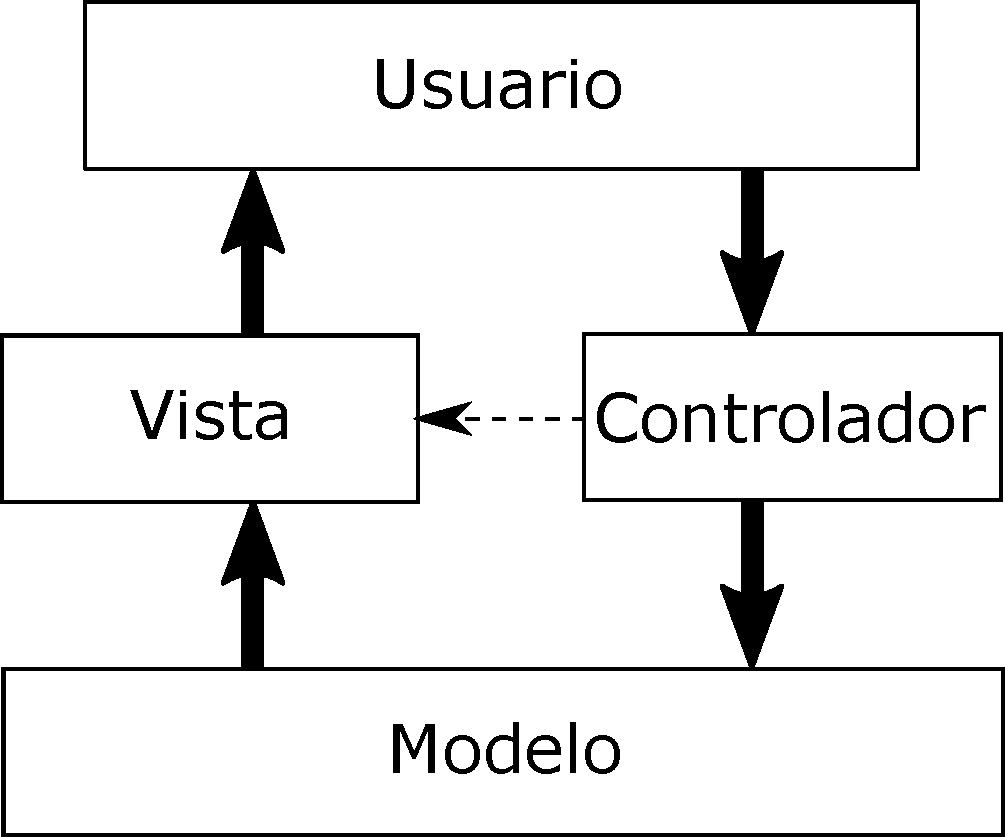
\includegraphics[width=\linewidth/2]{capitulo4/mvc}
		\par\end{centering}
	\smallskip
	\caption{\label{fig:mvc} Relación entre la vista, el modelo y el controlador.}
\end{figure} 

\smallskip

\begin{description}
	\item[Vista] Reúne los elementos que van a proporcionar al usuario la información que requiere.
	\item[Controlador] Comprende los módulos a los que el usuario acudirá para manipular el sistema. Eventualmente, después de realizar una operación, puede llamar a la vista para realimentar de información al usuario. 
	\item[Modelo] Contiene los componentes más internos, abstrayendo a la vista y al controlador de la representación de los datos o la interacción con el sistema.
\end{description}

Considerando los casos de uso y los requisitos, hemos enmarcado en el esquema modelo-vista-controlador los siguientes elementos:

\smallskip

\begin{figure}[H]
	\noindent \begin{centering}
		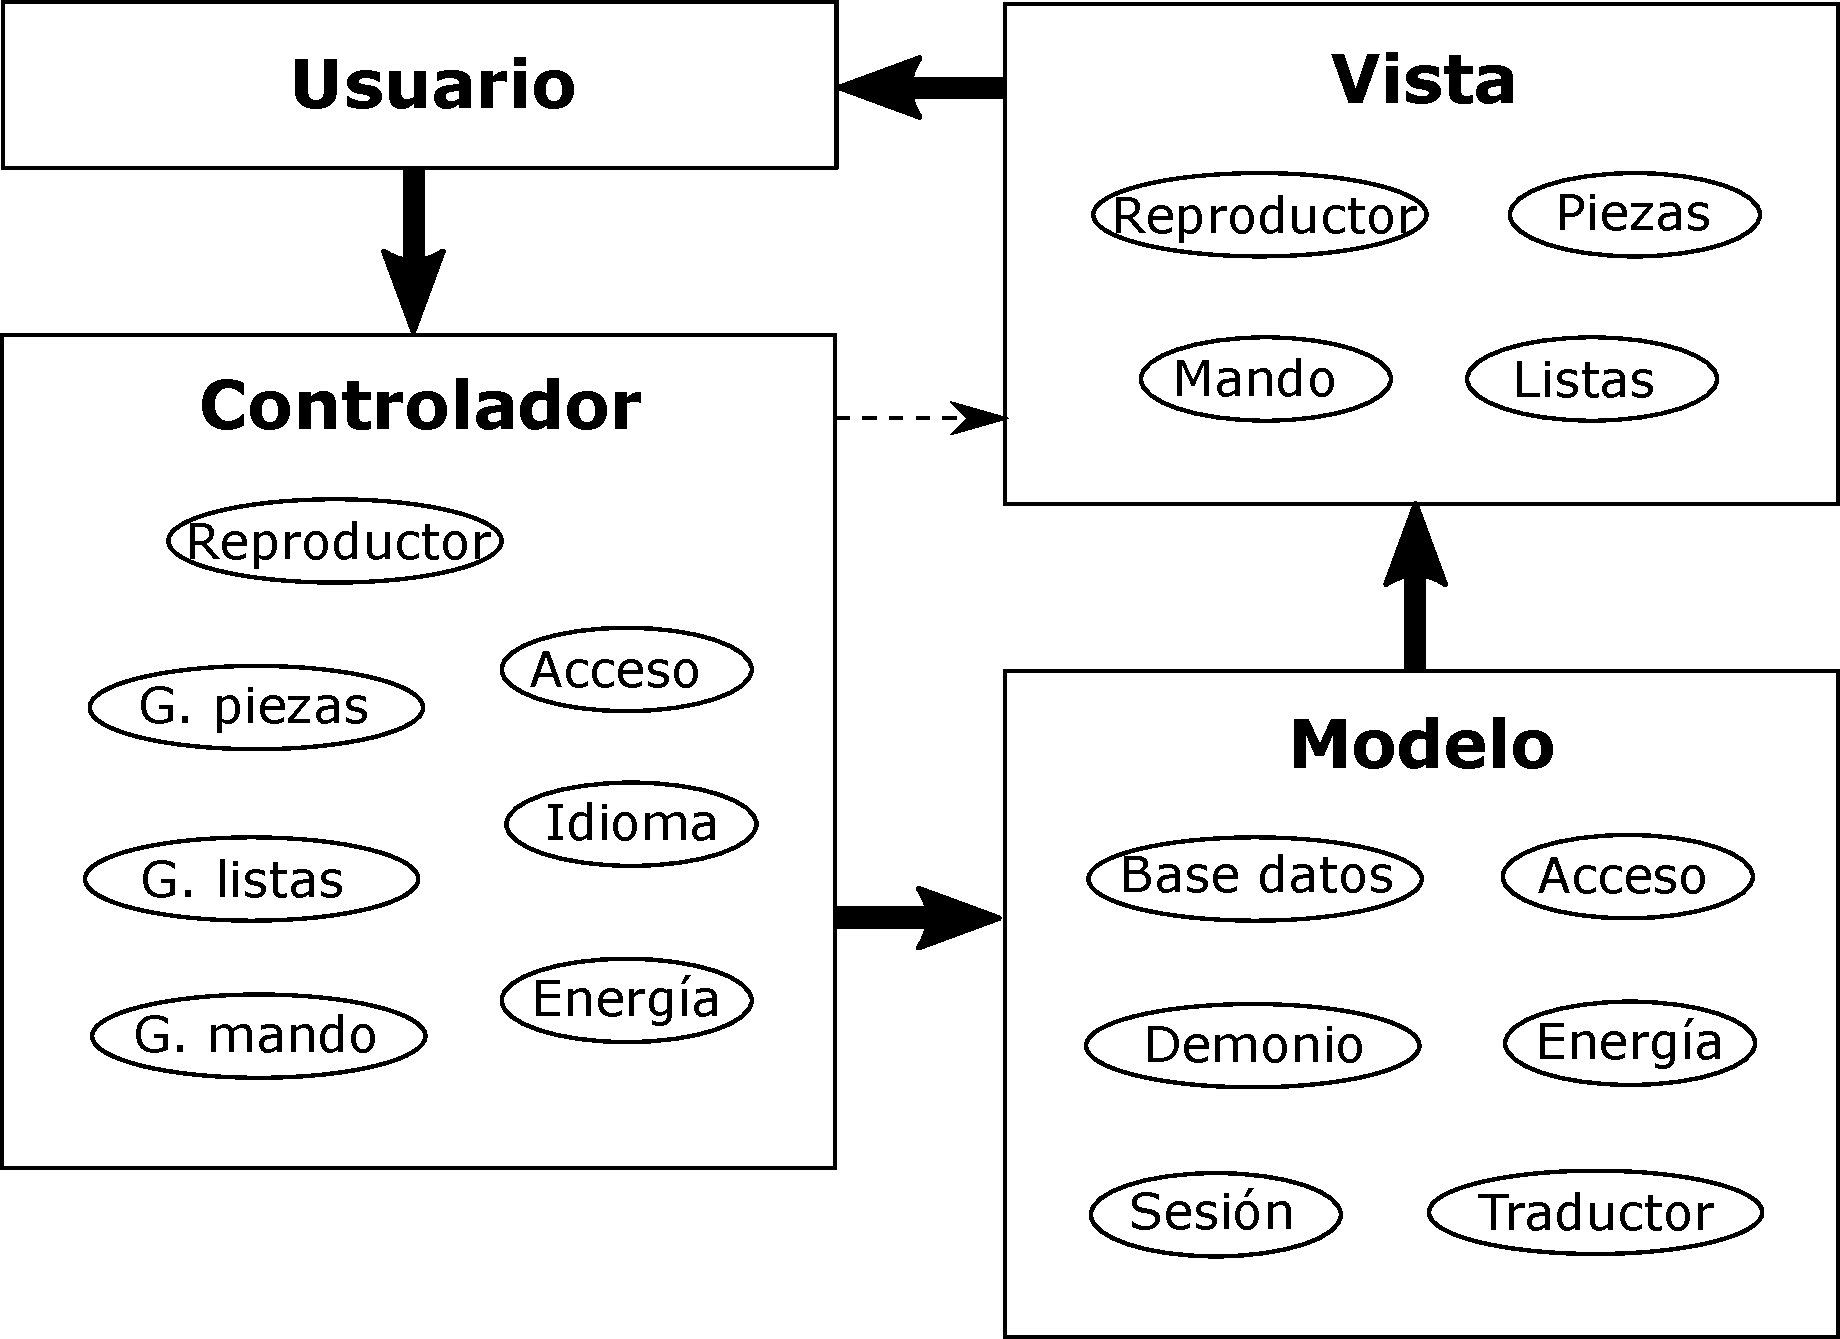
\includegraphics[width=\linewidth*2/3]{capitulo4/mvc_completo}
		\par\end{centering}
	\smallskip
	\caption{\label{fig:mvc_completo} Módulos que componen el sistema.}
\end{figure} 

\smallskip

A lo largo de esta sección detallaremos el comportamiento de todos los componentes.

\subsection{Estilo de la interfaz}

La visualidad es un punto importante en el diseño de interfaces gráficas, es la encargada de proporcionar una experiencia de usuario y hacer asequible la utilización del sistema. Pretendemos entregar la información requerida de forma clara y concisa, disponer fácilmente de los controles que puedan ser necesarios en cada vista, y que el estilo sea agradable y acorde a la solución que se está diseñando.

Por ello, vamos a fijarnos en la guía de estilo \textit{Material Design} de \textit{Google} \cite{material} para inspirarnos. La idea es sencilla: cada elemento de la interfaz se entiende como una hoja de papel. El diseñador maquetará la interfaz en base a hojas que se solapan, produciendo una sutil sombra cuando esto ocurre.

\textit{Material design} provee una gran cantidad de componentes de control y paletas de colores. De todos ellos, escogeremos listas, menús desplegables y botones flotantes. Nos decantamos por un color marrón, que evoca tranquilidad y estabilidad, dando idea de un \textit{software} intuitivo y robusto.

Una vez dibujados los primeros trazos, no es necesario maquetar completamente la interfaz con una aplicación para manipular imágenes, pudiendo diseñar las vistas en \acrshort{HTML} y \acrshort{CSS}, aún sin código de programación. Pero es muy útil dibujar al menos una página que nos sirva de plantilla. La siguiente imagen es una primera versión de la maqueta, diseñada con \textit{Adobe Photoshop}:

\smallskip

\begin{figure}[H]
	\noindent \begin{centering}
		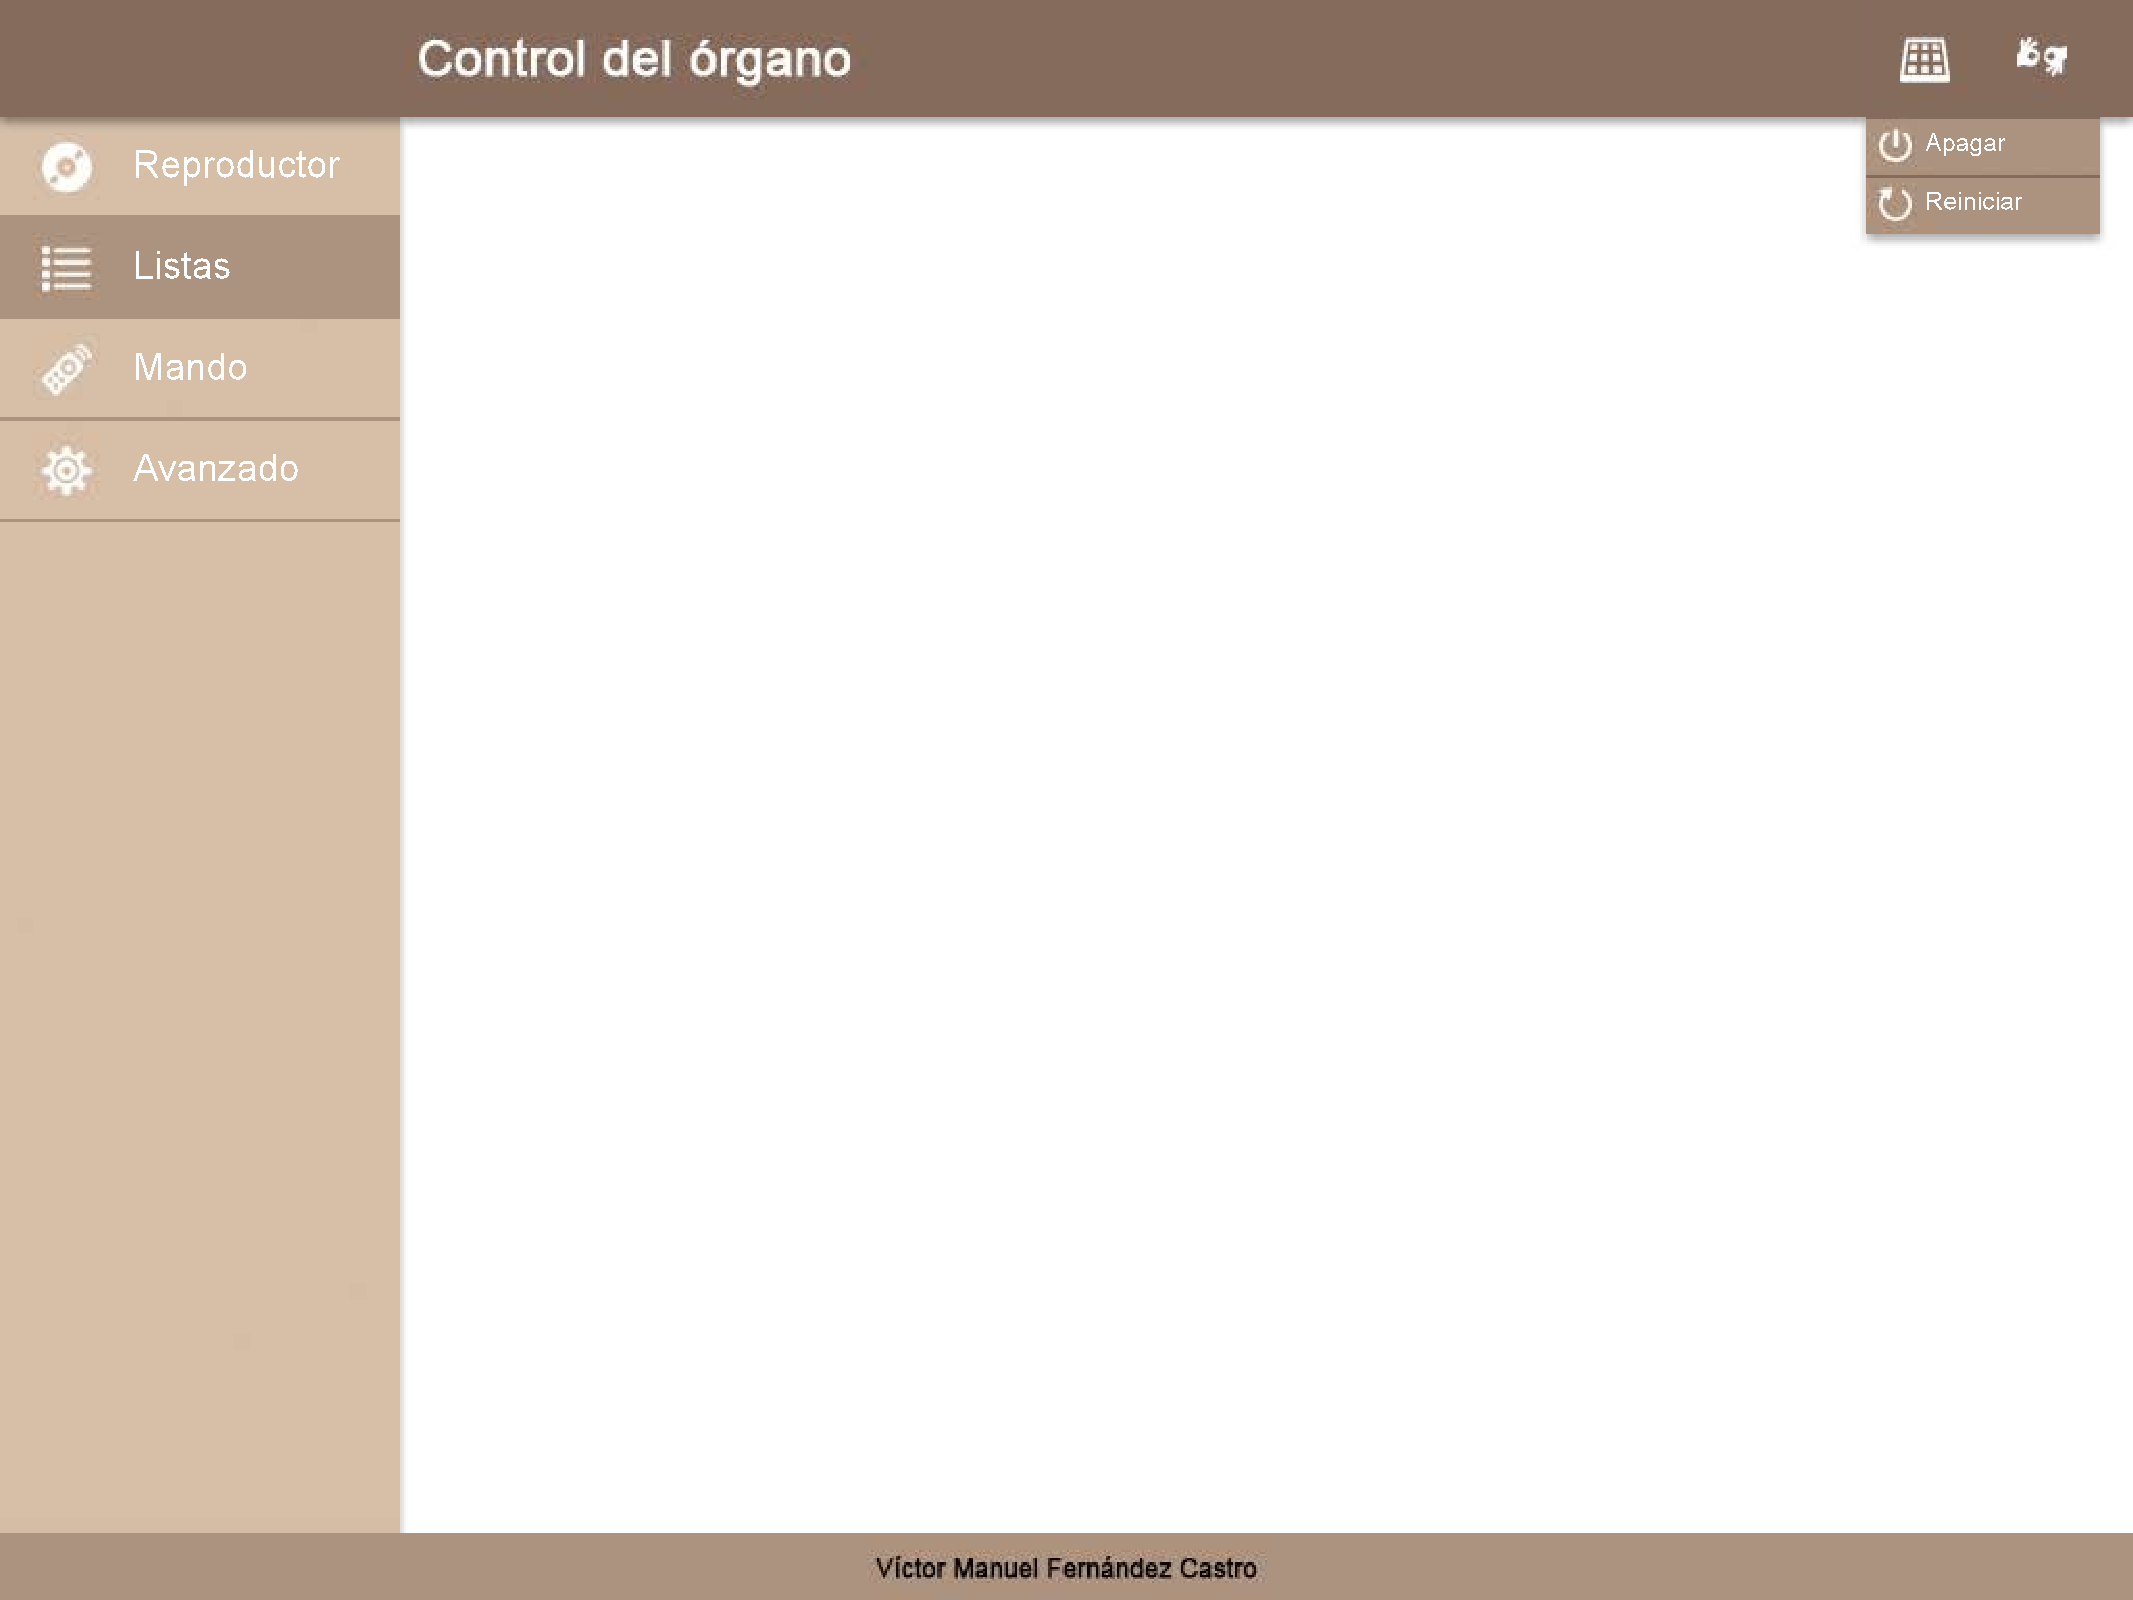
\includegraphics[width=\linewidth*3/4]{capitulo4/maqueta}
		\par\end{centering}
	\smallskip
	\caption{\label{fig:maqueta} Maquetación de las capas.}
\end{figure}

\smallskip

\subsection{Portada}
\label{subsec:portada}

La portada es la vista principal y va a cumplir dos funciones:

\begin{enumerate}
	\item Presentar la aplicación y dar la bienvenida.
	\item Introducir una contraseña para acceder al sistema.
\end{enumerate}

\subsubsection{Autentificación}

El módulo de autentificación recibe la contraseña introducida por el usuario, y utiliza la interfaz del modelo para validarla.

La contraseña será la de un usuario (a especificar) del sistema Linux, que provee una forma segura de almacenar contraseñas cifradas y gestionar usuarios. La verificación no se hará directamente, sino que llamaremos a un programa externo, que describiremos más abajo, en la sección \ref{subsec:applogin}, para que haga tal trabajo.

El resto de vistas y controladores de la interfaz deberán consultar si se ha iniciado sesión antes de proceder a realizar la petición correspondiente. Cuando un usuario accede al sistema con una contraseña válida, se guardará una marca en su sesión para no tener que introducirla en cada vista.


\subsubsection{Maqueta}

La vista proporcionará un fondo dinámico, con varias imágenes temáticas, y un cuadro para introducir la contraseña. Al hacerlo, se enviará al controlador, que se ocupará de verificar que la clave es correcta y concederá el acceso al reproductor.

\smallskip

\begin{figure}[H]
	\noindent \begin{centering}
		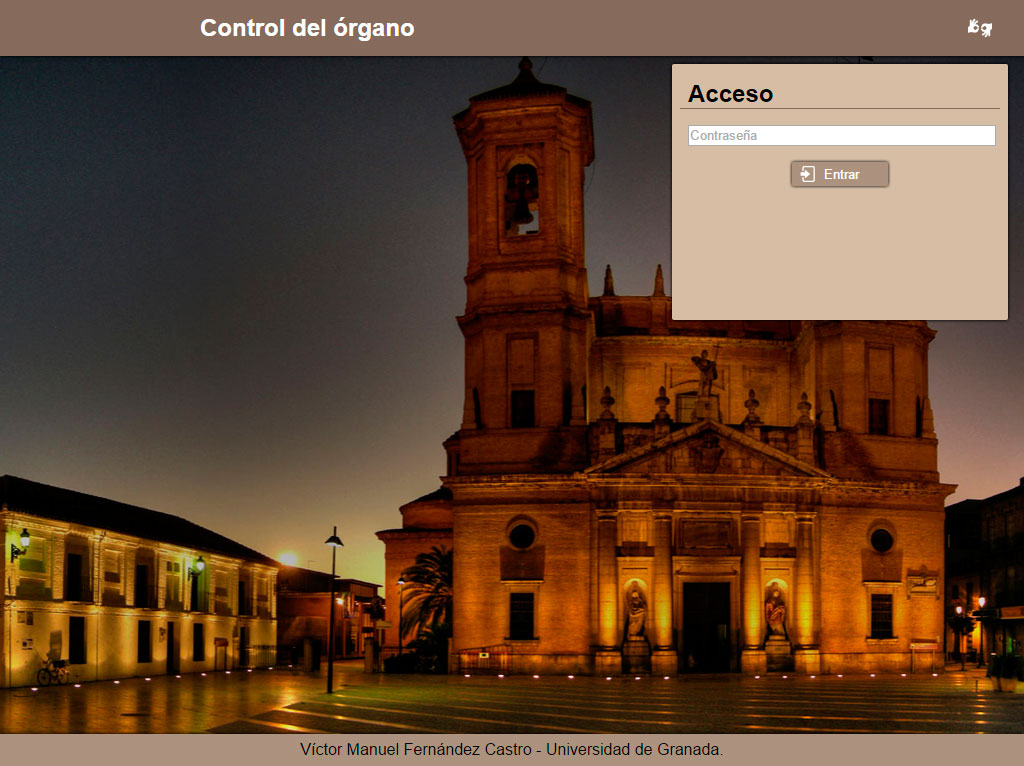
\includegraphics[width=\linewidth*3/4]{capitulo4/cap_portada}
		\par\end{centering}
	\smallskip
	\caption{\label{fig:cap_portada} Maqueta de la portada.}
\end{figure}

\smallskip

\subsubsection{Funciones}

Definiremos las siguientes funciones:

\begin{description}[style=nextline]
	\item[login (password)]
	Comprueba la contraseña llamando a una aplicación que diseñaremos específicamente.
	
	\begin{description}
		\item[password] Clave introducida por el usuario.
	\end{description}
	
	Si la contraseña es correcta, marca la autorización en la sesión y redirige a la vista del Reproductor. Si no, redirige a la portada y muestra un mensaje de error.
	
	\item[logout ()]
	Cierra la sesión retirando la marca de autorización de la sesión. Redirige a la portada.
	
\end{description}

\subsubsection{Diagrama de uso}

A continuación mostramos el diagrama de uso de la vista de portada y el módulo de acceso:

\smallskip

\begin{figure}[H]
	\noindent \begin{centering}
		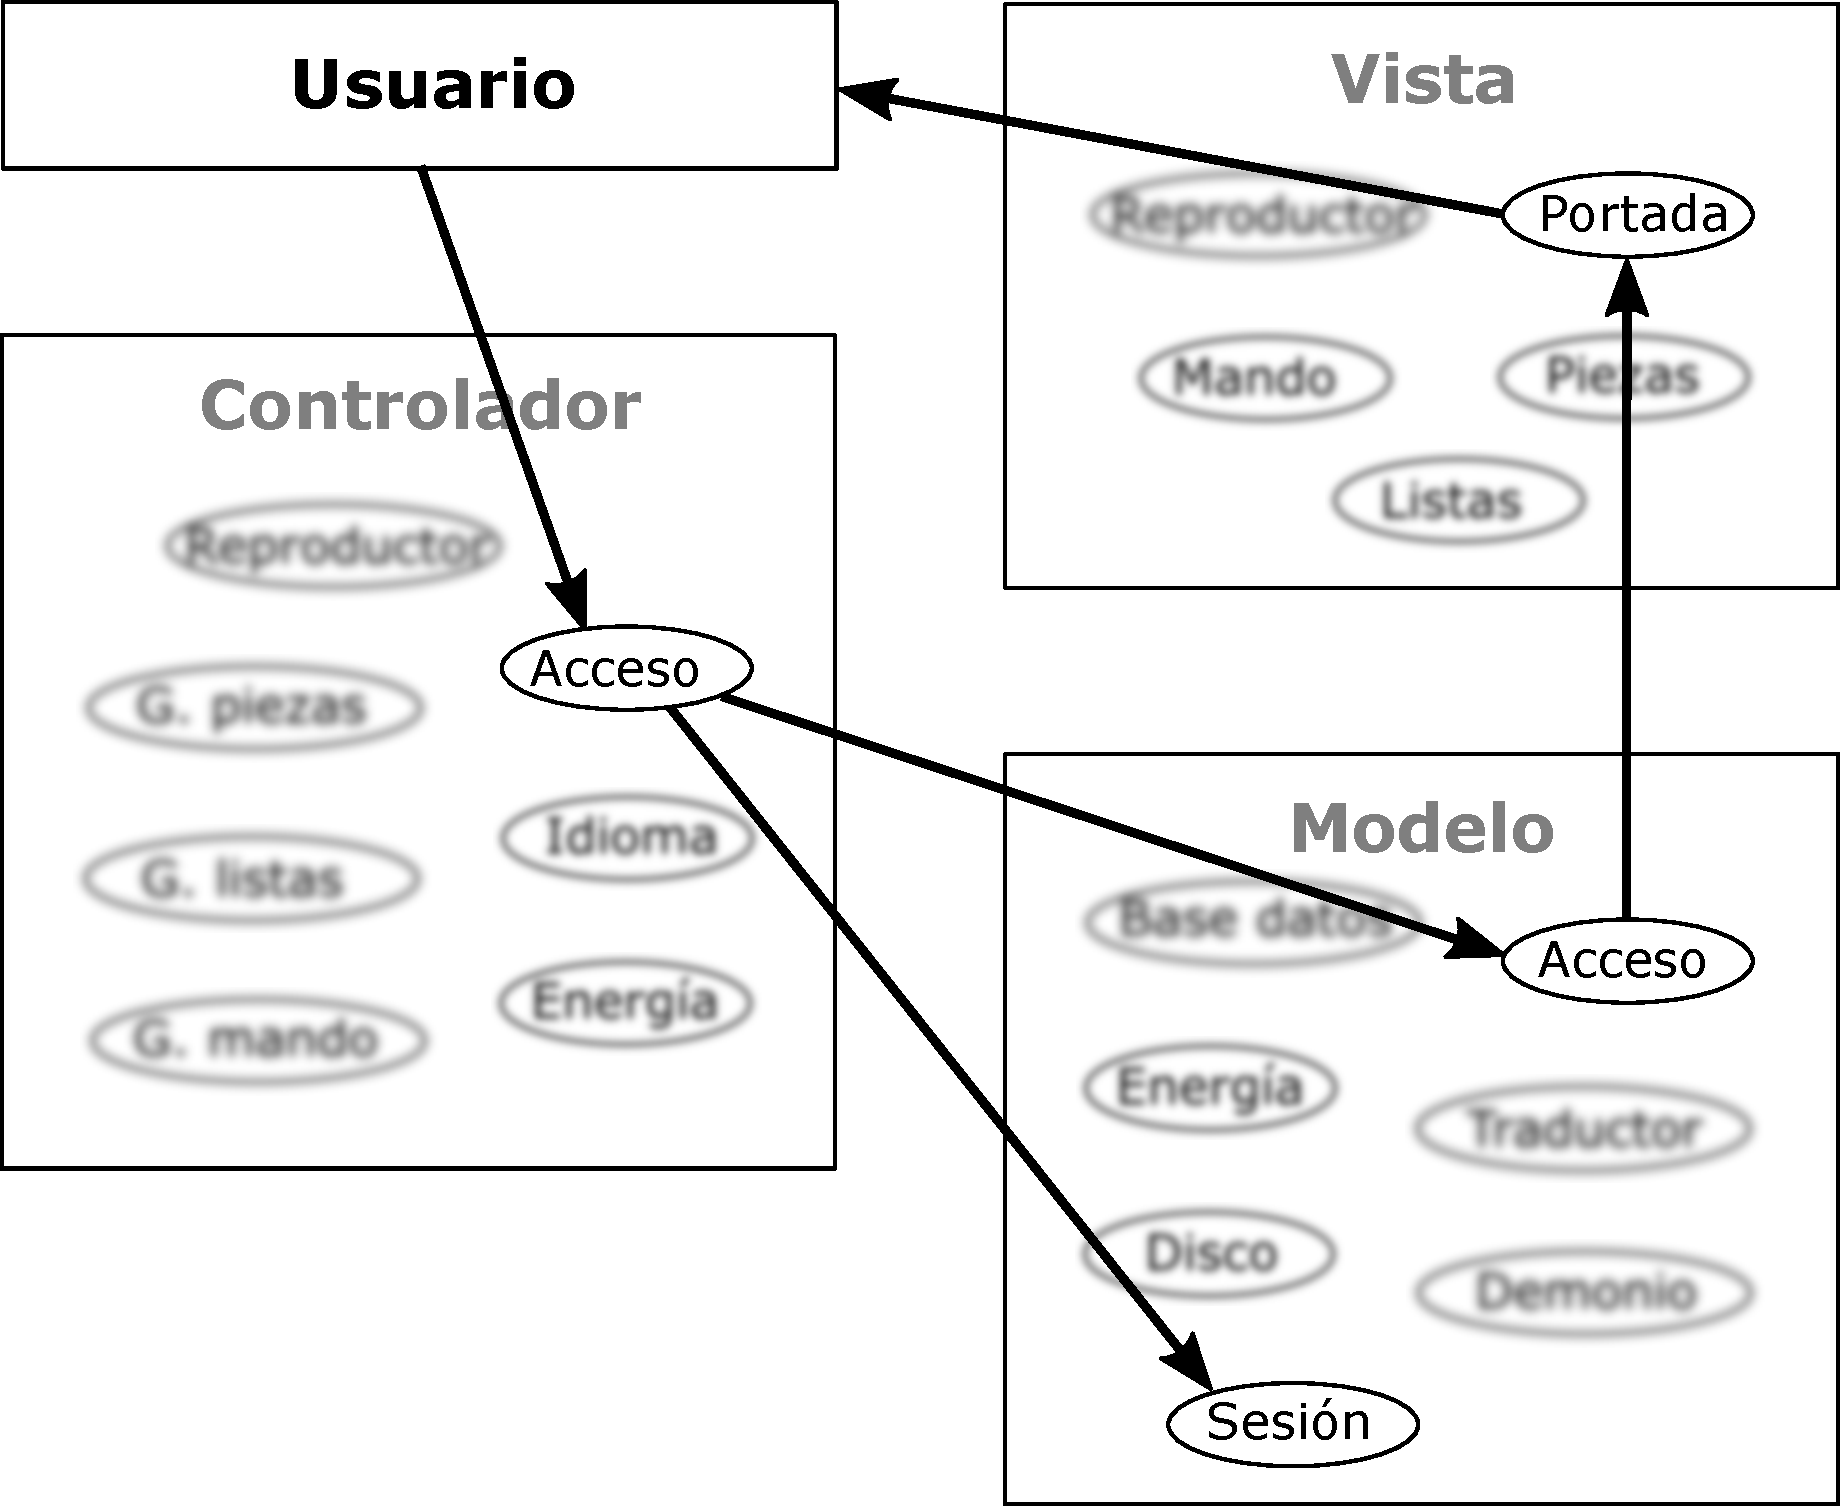
\includegraphics[width=\linewidth/2]{capitulo4/mvc_acceso}
		\par\end{centering}
	\smallskip
	\caption{\label{fig:mvc_acceso} Módulos implicados en el acceso al sistema.}
\end{figure} 

\smallskip

\subsection{Reproductor}

El reproductor es la parte fundamental de la interfaz. Mostrará los siguientes elementos:

\begin{enumerate}
	\item Estado del demonio (reproduciendo, pausado o detenido).
	\item Nombre de la pieza que se está ejecutando (si procede).
	\item Lista de reproducción activa (si procede).
	\item Controles de reproducción:
	
	\begin{enumerate}
		\item Pausar.
		\item Reanudar.
		\item Detener.
		\item Siguiente pieza.
		\item Pieza anterior.
	\end{enumerate}
\end{enumerate}

Hay que tener en cuenta que el protocolo de comunicación establece que el reproductor del demonio no es consciente de la lista de reproducción en la base de datos. Al ordenar una reproducción se le envía los nombres de archivo, como se describe en la función \textit{player\_playlist()} del demonio. De igual forma, al consultar el estado, devuelve el nombre de la pieza que se está ejecutando, cuya lista se puede conocer por reunión natural en la base de datos, y si no se encuentra, es porque se está reproduciendo un archivo externo, o tal vez otro usuario la ha eliminado.

Esto se hace así para evitar mantener un estado común entre el demonio y la interfaz, que podría provocar incoherencias si el cliente se desconecta repentinamente o si hay varios usuarios conectados al mismo tiempo.

\subsubsection{Maqueta}

Guiados por la lista de controles requeridos y la filosofía de \textit{Material Design}, proponemos la siguiente interfaz visual:

\smallskip

\begin{figure}[H]
	\noindent \begin{centering}
		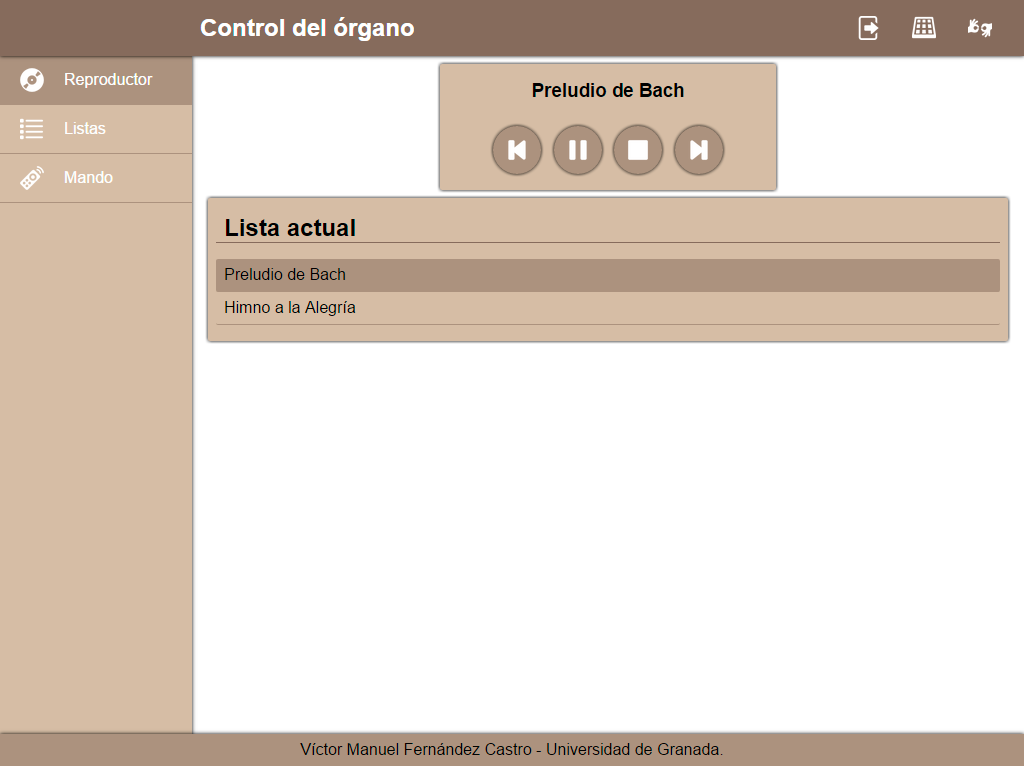
\includegraphics[width=\linewidth*3/4]{capitulo4/cap_reproductor}
		\par\end{centering}
	\smallskip
	\caption{\label{fig:cap_reproductor} Maqueta del reproductor.}
\end{figure} 

\smallskip

\subsubsection{Funciones}

Se definirán las siguientes funciones:

\begin{description}[style=nextline]
	\item[play (idplaylist, idscore)]
	Reproduce en bucle la lista indicada, empezando por la pieza especificada.
	
	\begin{description}
		\item[idplaylist] ID de la lista en la base de datos.
		\item[idscore] (opcional) ID de la primera pieza a reproducir.
	\end{description}
	
	Redirige a la vista del Reproductor.
	
	\item[pause ()]
	Pausa la reproducción de la partitura.
	
	\item[resume ()]
	Reanuda la ejecución de la pieza.
	
	\item[stop ()]
	Detiene completamente la reproducción en el demonio.
	
\end{description}

\subsubsection{Diagrama de uso}

El reproductor interacciona con el resto de la interfaz según este esquema:

\smallskip

\begin{figure}[H]
	\noindent \begin{centering}
		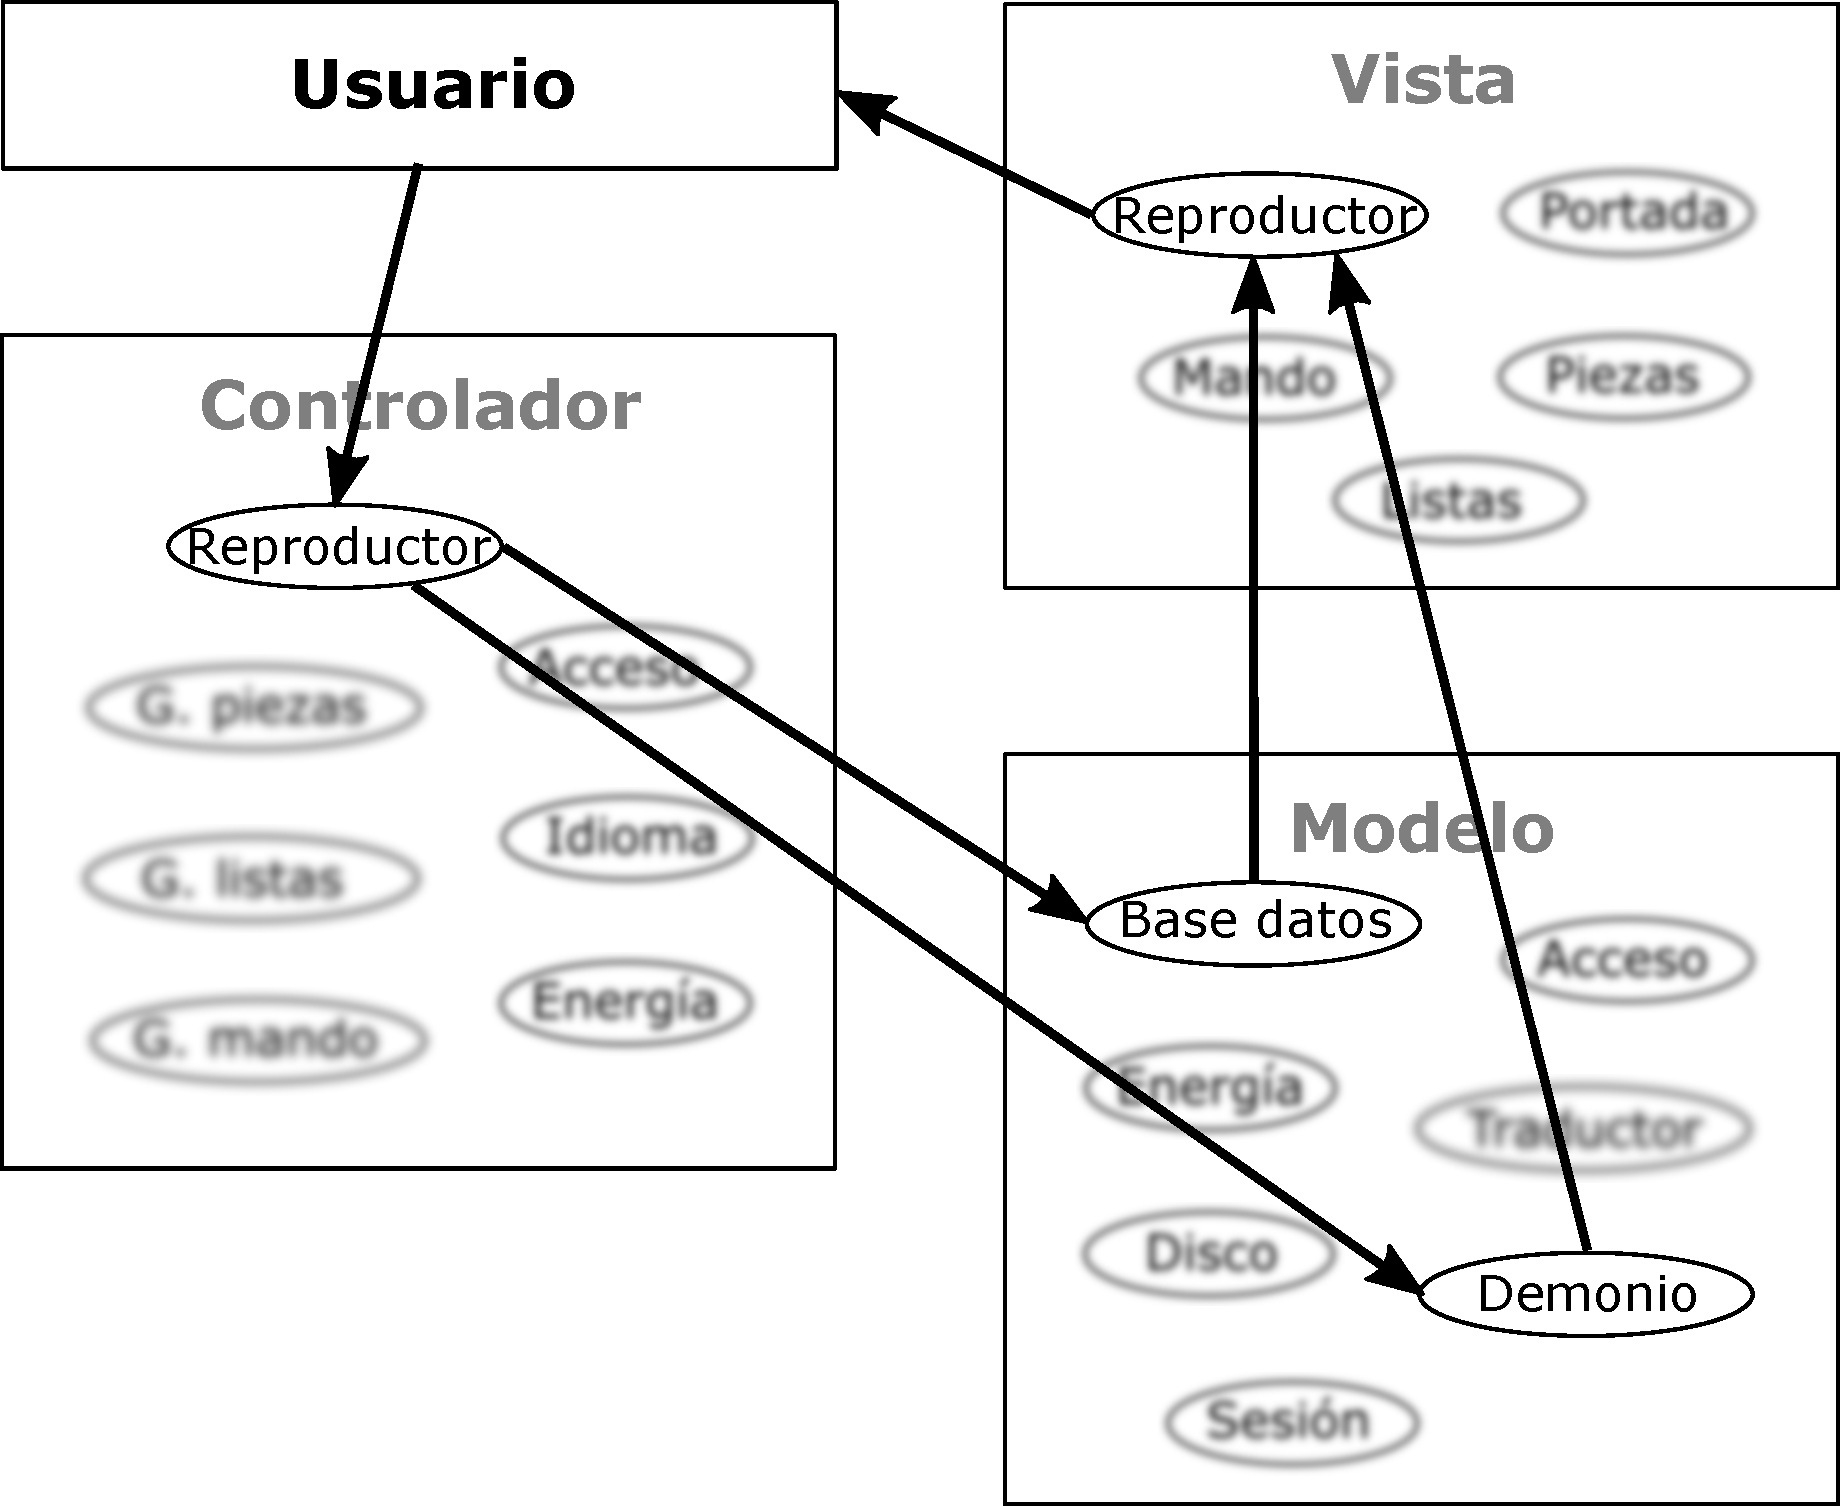
\includegraphics[width=\linewidth/2]{capitulo4/mvc_reproductor}
		\par\end{centering}
	\smallskip
	\caption{\label{fig:mvc_reproductor} Módulos implicados en el reproductor.}
\end{figure} 

\smallskip

\subsection{Gestión de listas de reproducción}

Una parte importante de la interfaz es facilitar la organización de la información. Las piezas musicales se clasificarán en listas de reproducción. Este módulo agrega la funcionalidad necesaria para gestionar listas.

El gestor se presentará con los siguientes controles:

\begin{enumerate}
	\item Lista de listas de reproducción, con el siguiente contenido:

	\begin{enumerate}
		\item Nombre de la lista.
		\item Número de piezas contenidas.
		\item Vínculo para acceder a la lista.
		\item Vínculo para ejecutar la lista en el reproductor.
	\end{enumerate}
	
	\item Botón para crear una nueva lista. Al dispararlo, abrirá un cuadro de diálogo para introducir el nombre de la lista.
	
\end{enumerate}

\subsubsection{Maqueta}

Hemos diseñado la vista de este módulo con el siguiente aspecto:

\smallskip

\begin{figure}[H]
	\noindent \begin{centering}
		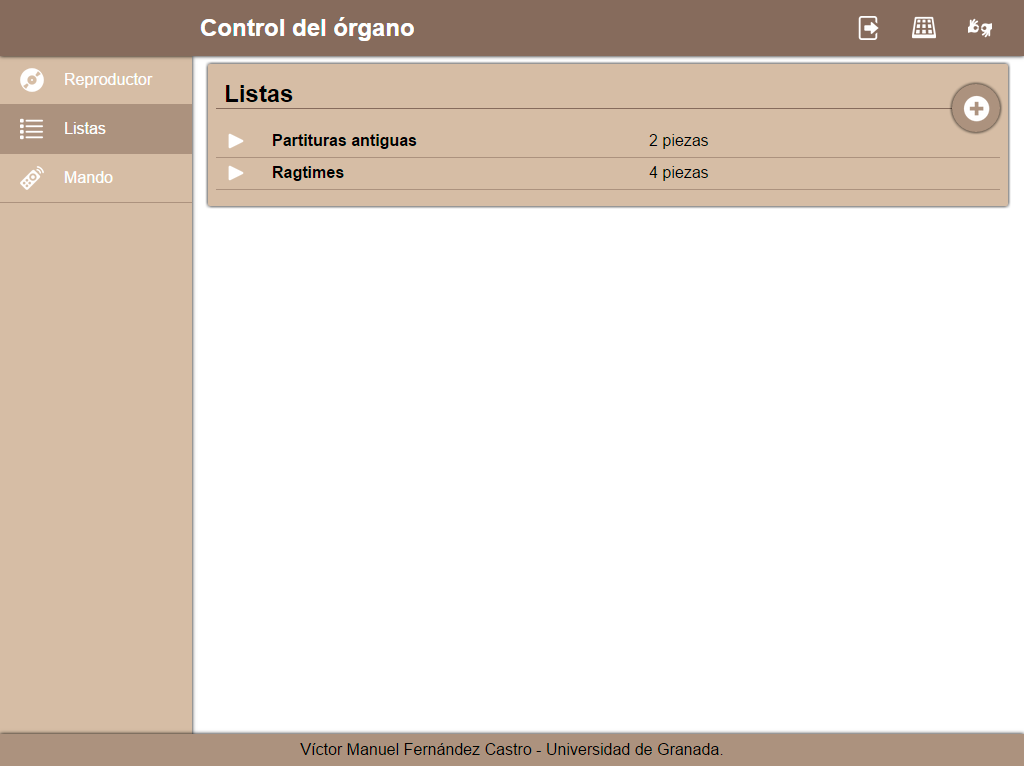
\includegraphics[width=\linewidth*3/4]{capitulo4/cap_listas}
		\par\end{centering}
	\smallskip
	\caption{\label{fig:cap_listas} Maqueta del gestor de listas de reproducción.}
\end{figure} 

\smallskip

\subsubsection{Funciones}

El controlador tendrá las siguientes funciones:

\begin{description}[style=nextline]
	\item[new\_playlist (name)]
	Genera una lista nueva, con el nombre que se recibe. 
	
	\begin{description}
		\item[name] Nombre que identificará a la nueva lista.
	\end{description}
	
	Redirige al administrador de la nueva lista.
	
	\item[rename\_playlist (idplaylist, name)]
	Cambia el nombre de una lista existente.
	
	\begin{description}
		\item[idplaylist] ID de la lista en la base de datos.
		\item[name] Nuevo nombre a asignar a la lista.
	\end{description}
	
	Redirige al administrador de la lista.
	
	\item[delete\_playlist (idplaylist)]
	Elimina una lista de reproducción y todas las partituras que contenga.
	
	\begin{description}
		\item[idplaylist] ID de la lista en la base de datos.
	\end{description}
	
	Redirige al gestor de listas de reproducción.
	
\end{description}

\subsubsection{Diagrama de uso}

Los componentes implicados en la gestión de listas se relacionan de la siguiente forma:

\smallskip

\begin{figure}[H]
	\noindent \begin{centering}
		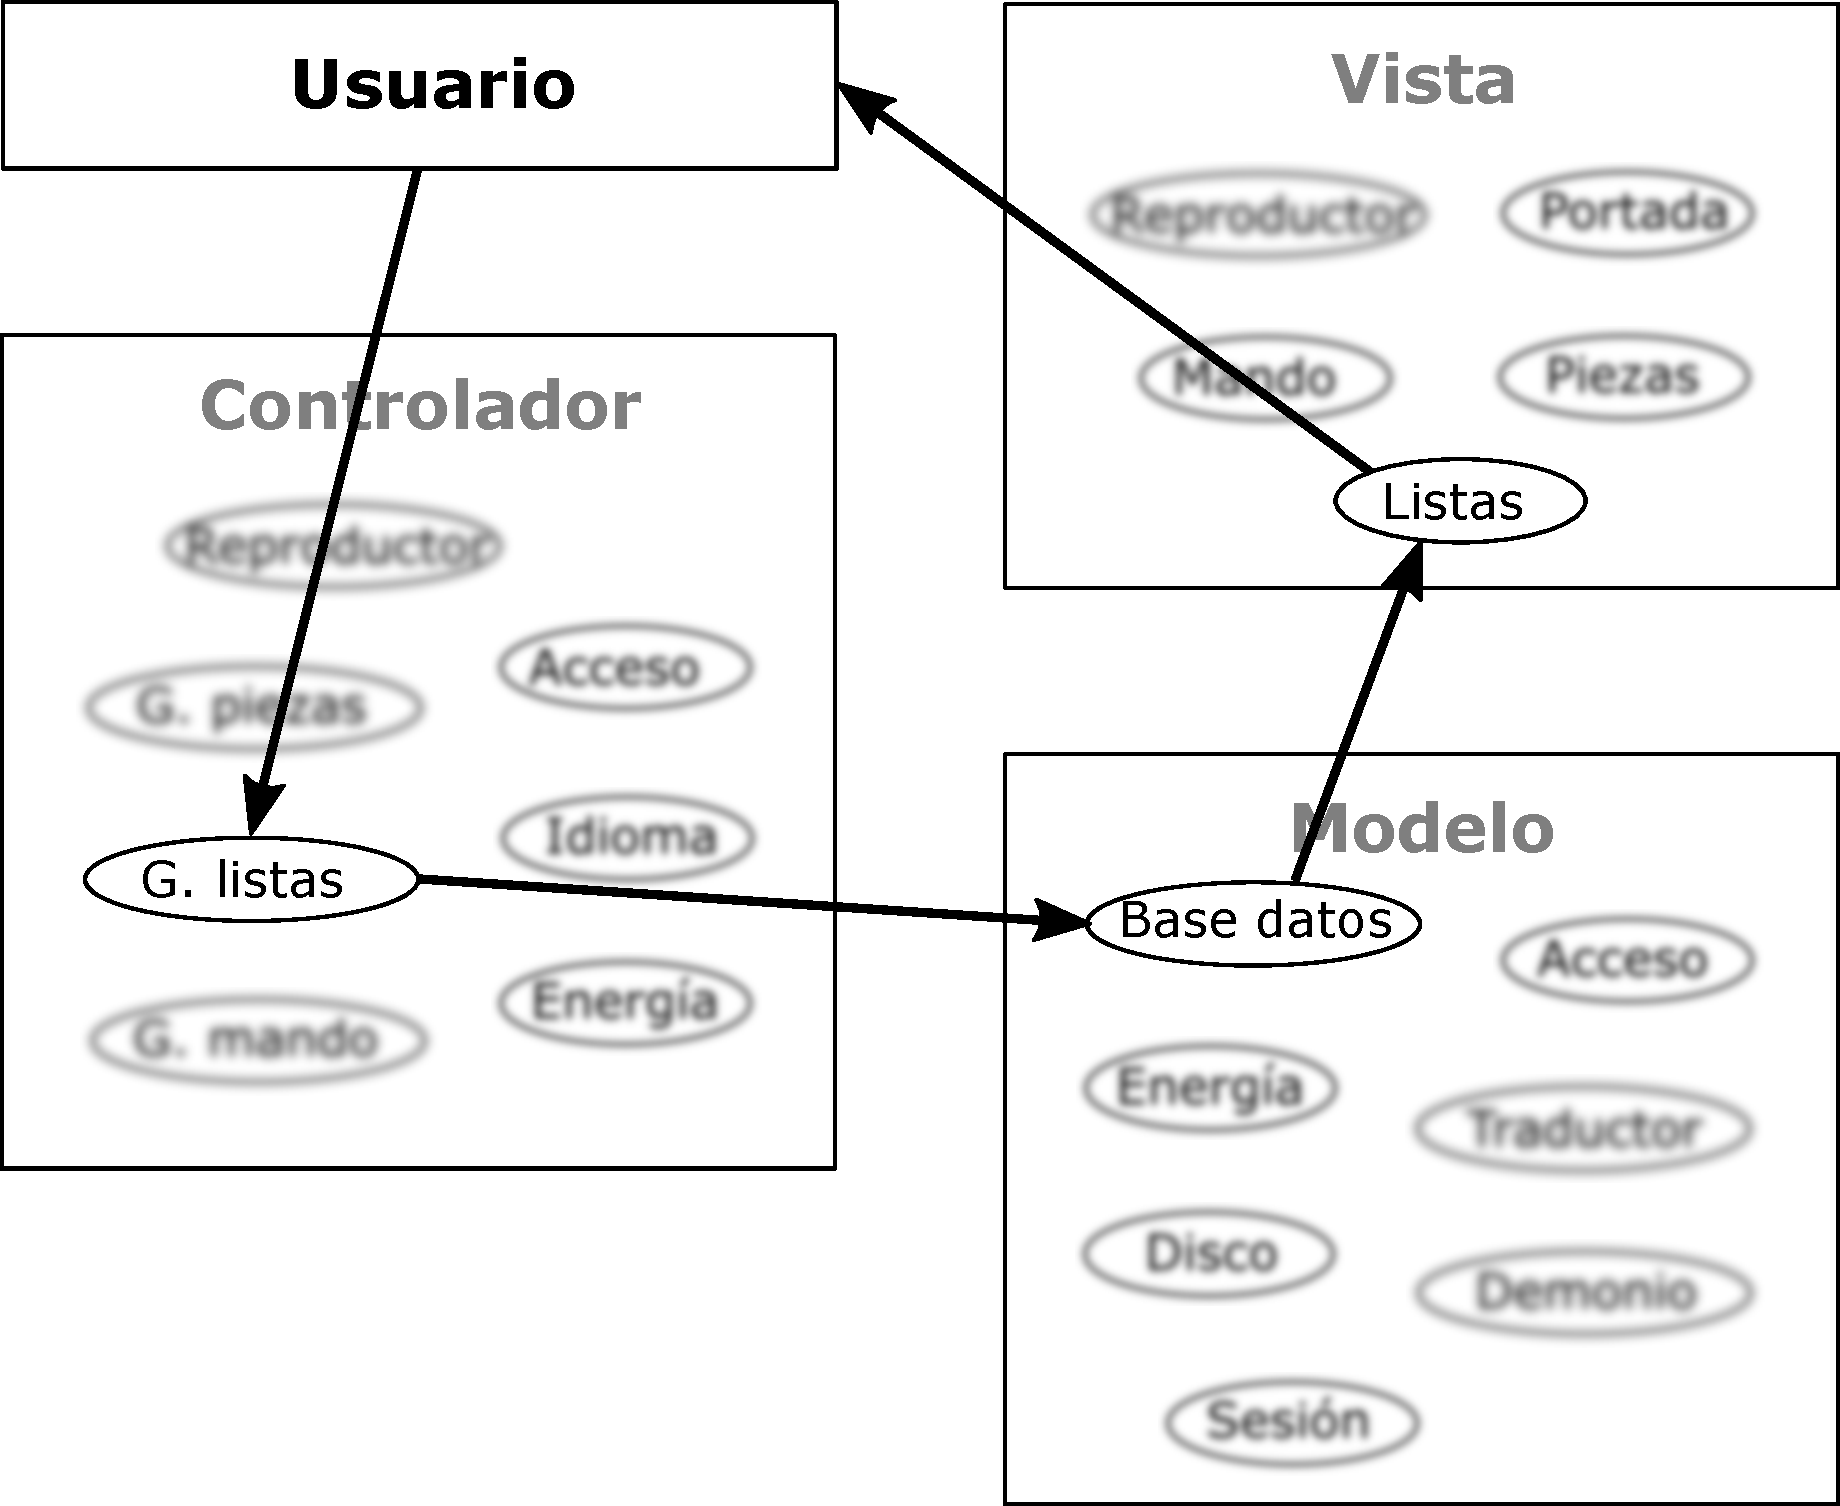
\includegraphics[width=\linewidth/2]{capitulo4/mvc_listas}
		\par\end{centering}
	\smallskip
	\caption{\label{fig:mvc_listas} Módulos implicados en el gestor de listas.}
\end{figure} 

\smallskip

\subsection{Gestión de partituras}
\label{subsec:piezas}

El gestor de partituras está estrechamente relacionado con el de listas de reproducción, en tanto que realmente es el gestor de una lista concreta. Desde aquí podremos conocer el contenido de cada lista, así como renombrarla y eliminarla. Al mismo tiempo, servirá para añadir partituras, cambiar su título y borrarlas, de una forma similar a las propias listas.

Los controles de la interfaz serán los siguientes:

\begin{enumerate}
	\item Editar el nombre de la lista que se está mostrando.
	\item Eliminar completamente la lista.
	\item Añadir una pieza a la lista.
	\item Control oculto para añadir una pieza arrastrando un fichero sobre la vista (\textit{drag \& drop}).
	\item Lista de partituras que contiene la lista, con el siguiente contenido:
	
	\begin{enumerate}
		\item Nombre de la pieza.
		\item Duración de la obra.
		\item Vínculo para reproducirla.
		\item Vínculo para descargarla en el cliente.
		\item Control para renombrar la partitura.
		\item Control para eliminar la pieza.
	\end{enumerate}
\end{enumerate}

\subsubsection{Maqueta}

Todos los controles se dispondrán de la siguiente forma:

\smallskip

\begin{figure}[H]
	\noindent \begin{centering}
		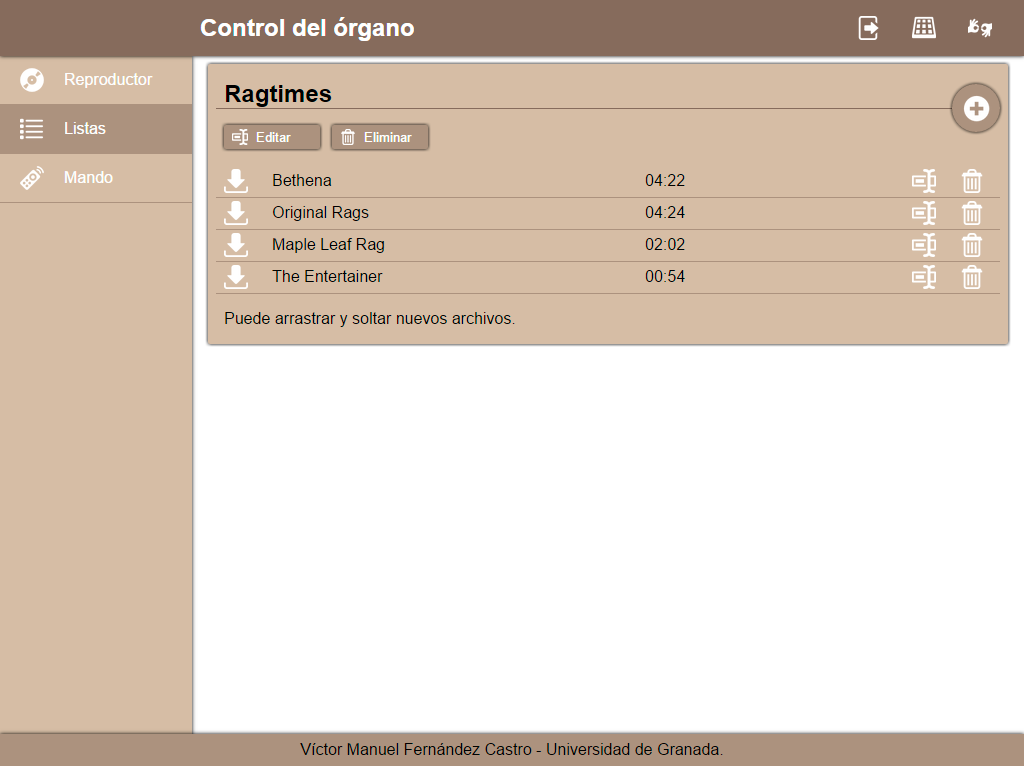
\includegraphics[width=\linewidth*3/4]{capitulo4/cap_piezas}
		\par\end{centering}
	\smallskip
	\caption{\label{fig:cap_piezas} Maqueta del gestor de piezas musicales.}
\end{figure} 

\smallskip

\subsubsection{Funciones}

Para hacer funcionar este módulo son necesarios los siguientes procedimientos:

\begin{description}[style=nextline]
	\item[new\_score (idplaylist, name, score)]
	Inserta una pieza en la lista de reproducción y guarda el archivo en el almacenamiento interno. Para conocer la duración de una partitura, hace una llamada a lun aplicación que diseñaremos para extraer información de archivos \acrshort{MIDI} (véase la sección \ref{subsec:midinfo}).
	
	\begin{description}
		\item[idplaylist] ID de la lista de reproducción que contendrá la partitura.
		\item[name] Nombre que identificará a la nueva obra.
		\item[score] Fichero de formato \acrshort{MIDI} que contiene la pieza.
	\end{description}
	
	Redirige al administrador de la lista contenedora.
	
	\item[rename\_score (idscore, name)]
	Cambia el nombre de una pieza existente.
	
	\begin{description}
		\item[idscore] ID de la partitura en la base de datos.
		\item[name] Nuevo nombre a asignar a la pieza.
	\end{description}
	
	Redirige al administrador de la lista que contiene la partitura.
	
	\item[delete\_score (idscore)]
	Elimina una partitura de la base de datos y del almacenamiento.
	
	\begin{description}
		\item[idscore] ID de la pieza en la base de datos.
	\end{description}
	
	Redirige al gestor partituras que contenía a la pieza eliminada.
	
\end{description}

\subsubsection{Diagrama de uso}

La interacción entre los componentes implicados es la siguiente:

\smallskip

\begin{figure}[H]
	\noindent \begin{centering}
		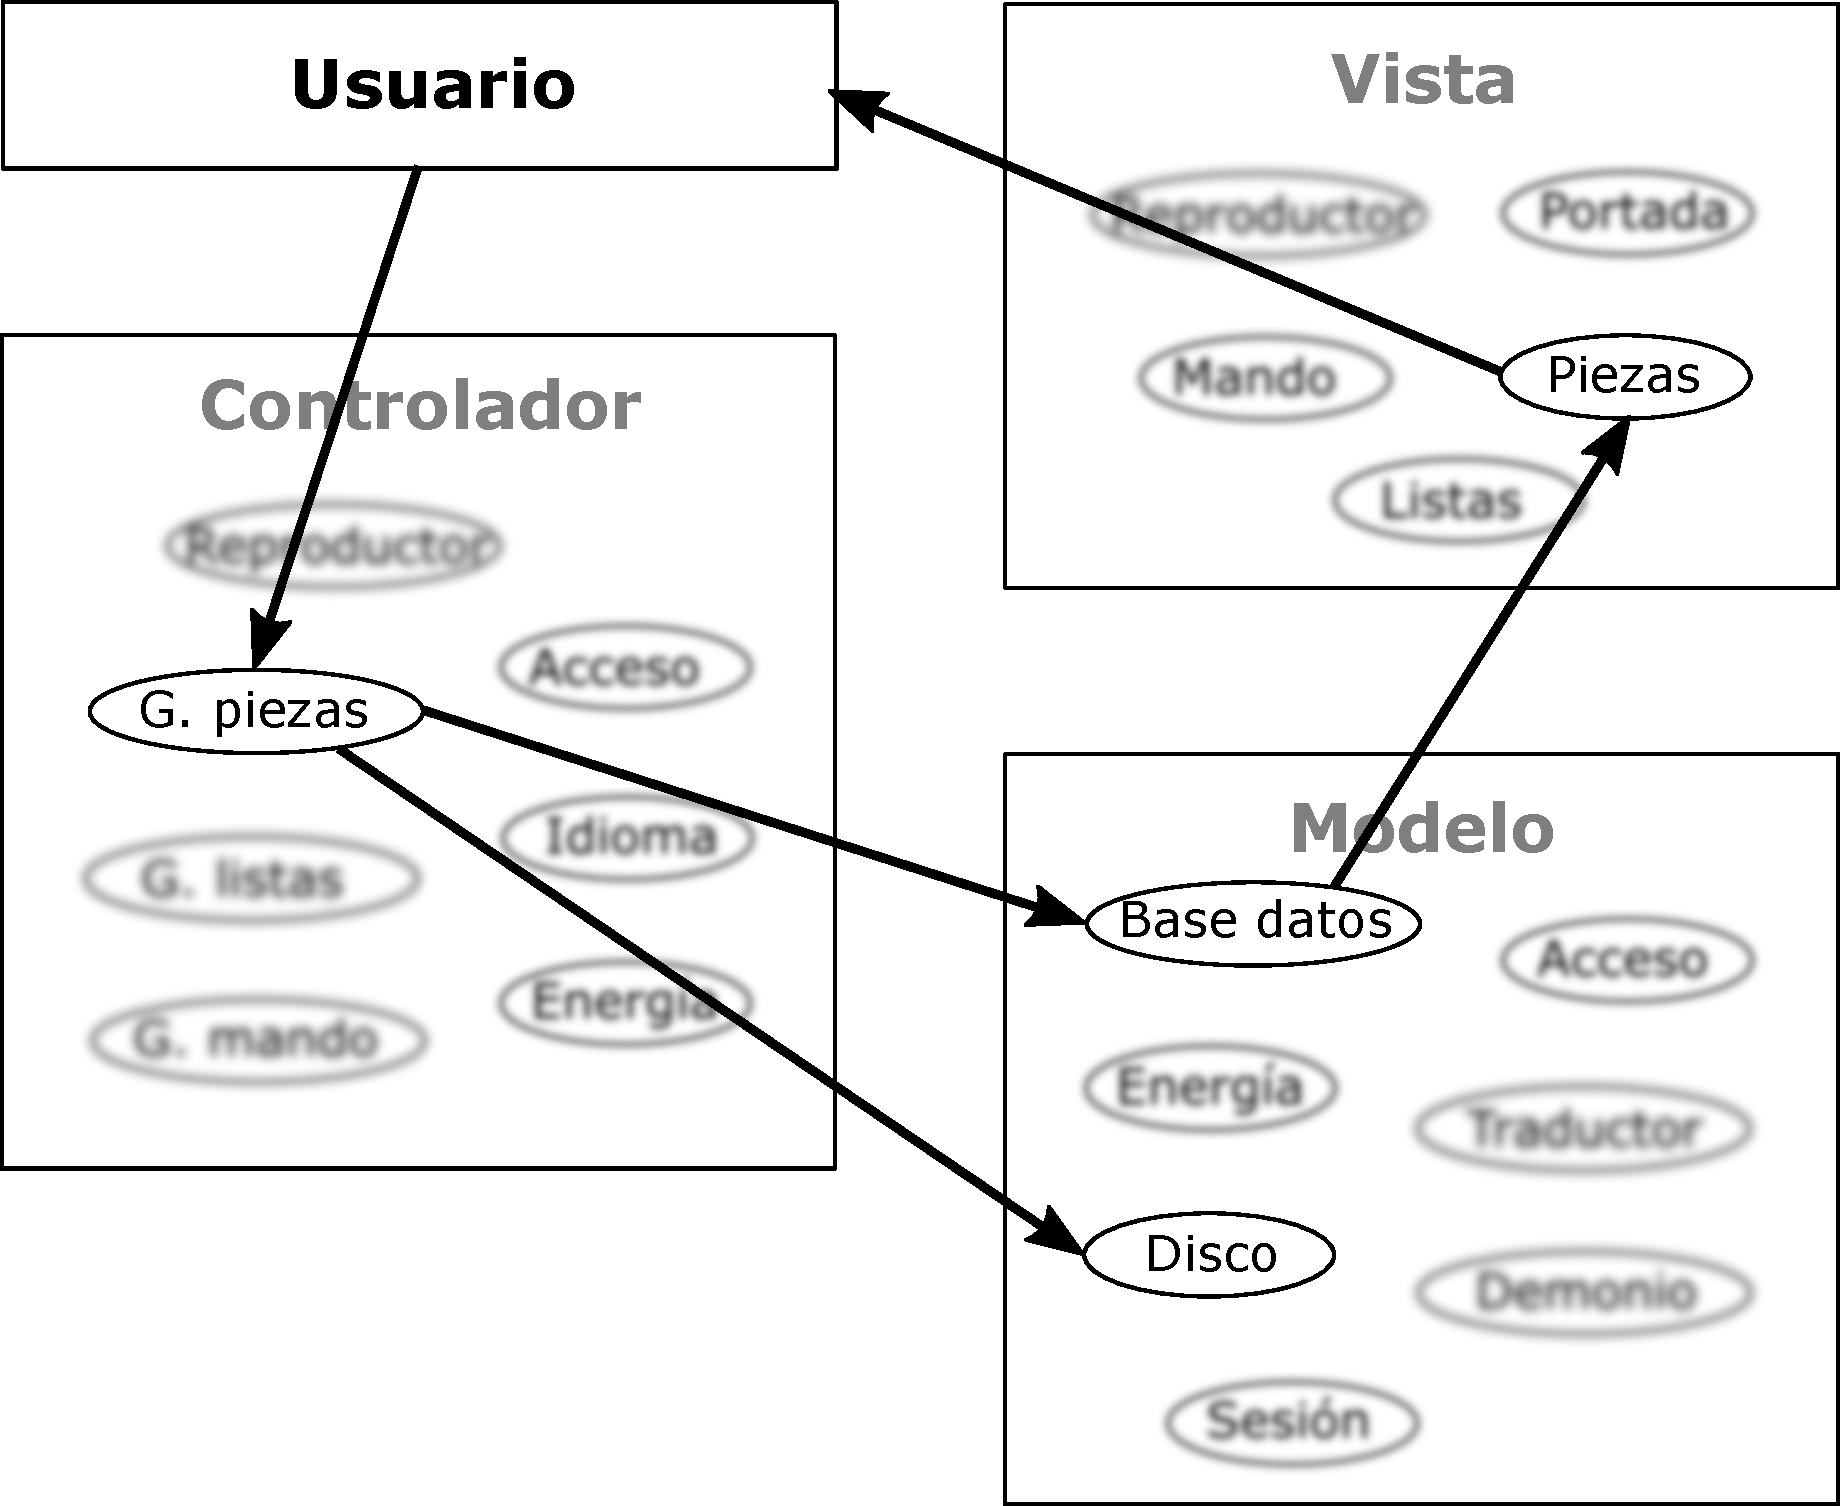
\includegraphics[width=\linewidth/2]{capitulo4/mvc_piezas}
		\par\end{centering}
	\smallskip
	\caption{\label{fig:mvc_piezas} Módulos implicados en el gestor de partituras.}
\end{figure} 

\smallskip

\subsection{Asignación del mando a listas}

Como ya sabemos, en base al diseño general, dispondremos de un mando a distancia que permitirá iniciar la reproducción de listas de partituras según una asignación que podrá realizar el usuario.

La adición o sustracción de botones compete al administrador del sistema, pero la asignación puede ser modificada por cualquier usuario. La interfaz es sencilla: se mostrará una lista de todos los botones disponibles, junto a un menú desplegable que presentará todas las listas existente, dando opción a escoger una de ellas, o ninguna.

Recordar que esta interfaz normalmente mostrará menos botones de los que tiene el mando, ya que se debe reservar al menos dos para pausar y detener la reproducción.

\subsubsection{Maqueta}

Esta es la vista de este componente:

\smallskip

\begin{figure}[H]
	\noindent \begin{centering}
		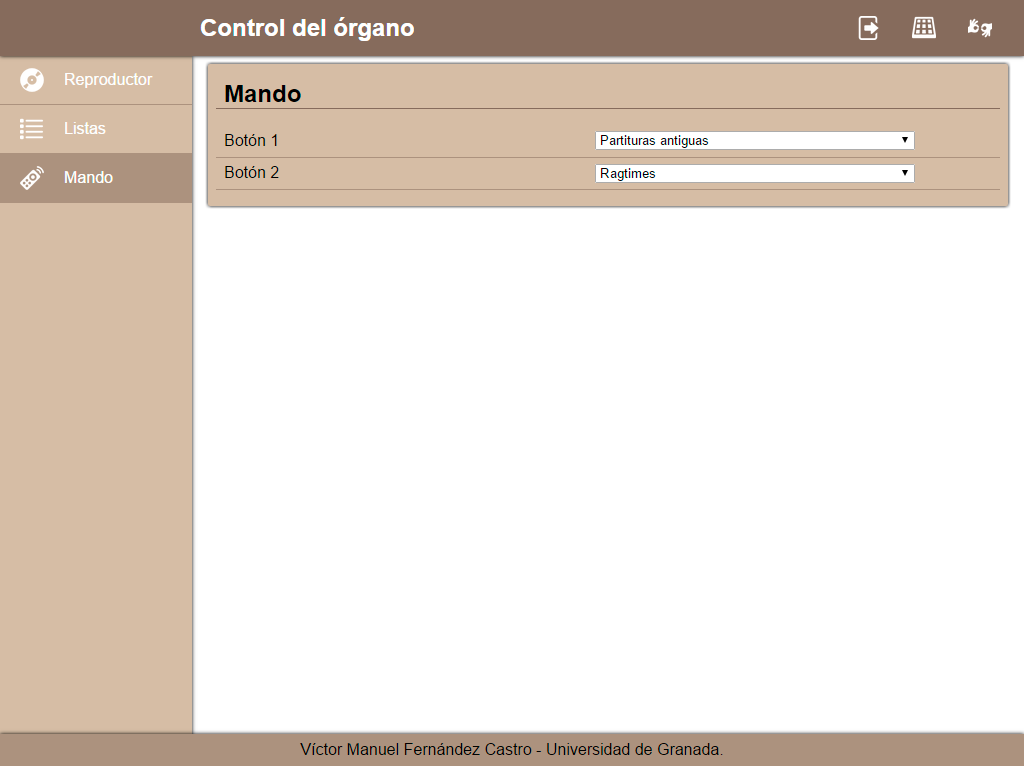
\includegraphics[width=\linewidth*3/4]{capitulo4/cap_mando}
		\par\end{centering}
	\smallskip
	\caption{\label{fig:cap_mando} Maqueta del gestor de botones del mando.}
\end{figure} 

\smallskip

\subsubsection{Funciones}

El controlador utilizará la siguiente función:

\begin{description}[style=nextline]
	\item[set\_shortcut (idshortcut, idplaylist)]
	Asignar una lista de reproducción a un botón del mando.
	
	\begin{description}
		\item[idshortcut] ID del botón del mando en la base de datos.
		\item[idplaylist] ID de la lista de partituras escogida. Puede ser un valor nulo.
	\end{description}
	
	Redirige a la vista del asignaciones del mando.
\end{description}

\subsubsection{Diagrama de uso}

El gestor de botones del mando relaciona sus componentes de la siguiente manera:

\smallskip

\begin{figure}[H]
	\noindent \begin{centering}
		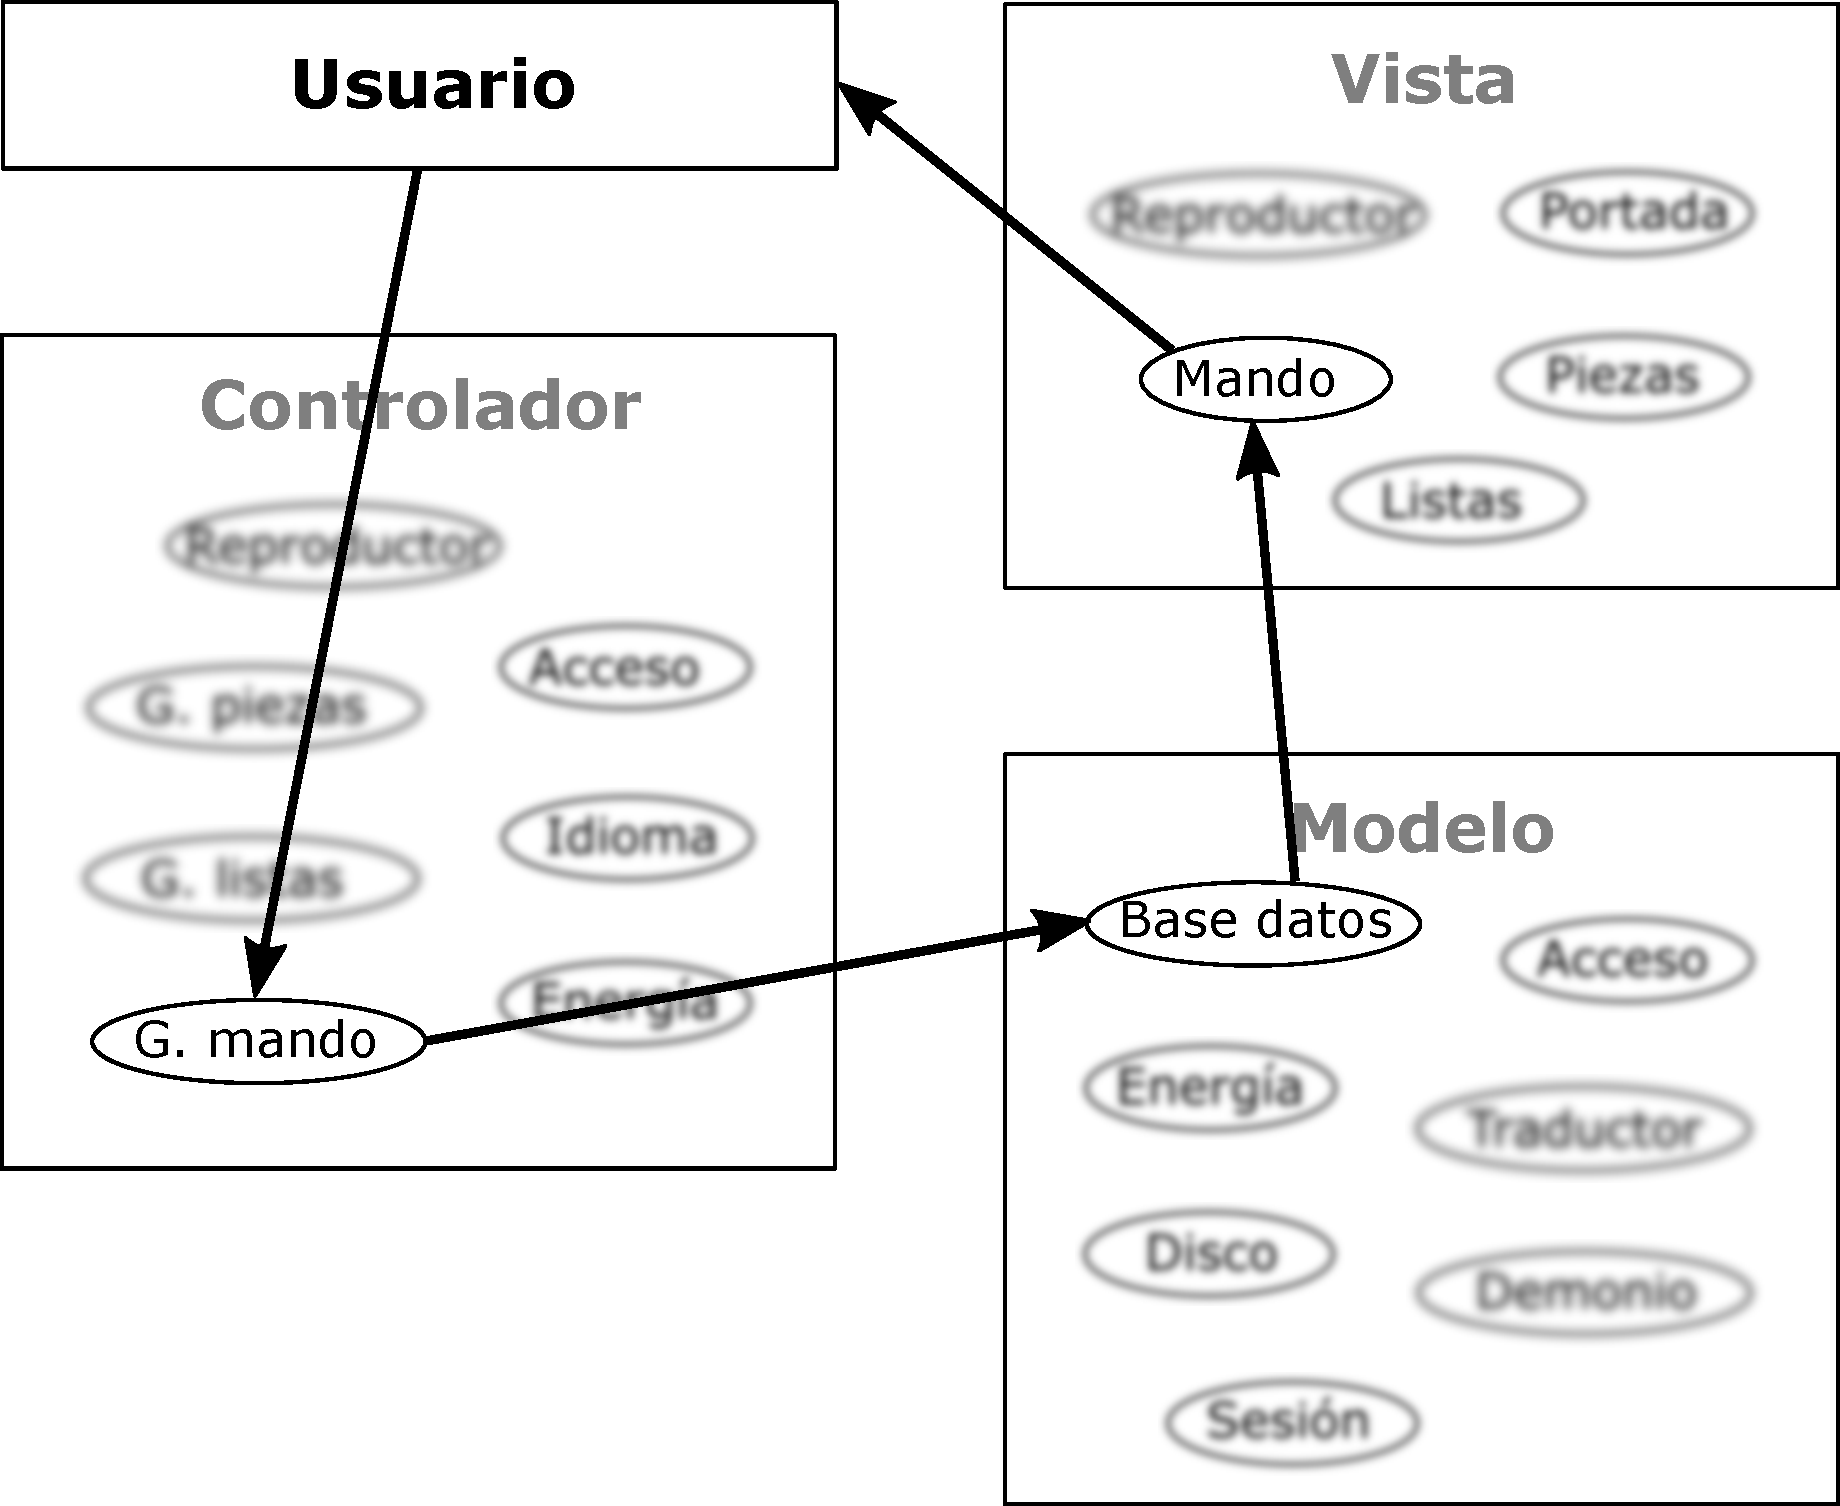
\includegraphics[width=\linewidth/2]{capitulo4/mvc_mando}
		\par\end{centering}
	\smallskip
	\caption{\label{fig:mvc_mando} Módulos implicados en el gestor del mando.}
\end{figure} 

\smallskip

\subsection{Control de energía}

Hemos contemplado proveer la posibilidad de apagar o reiniciar el sistema remotamente. Para ello, ofreceremos un menú en la cabecera de la pantalla, que será común a todas las vistas, excepto la portada, con el siguiente contenido:

\begin{enumerate}
	\item Apagar el sistema.
	\item Reiniciar el sistema.
\end{enumerate}

El control de energía es una operación de control, no de vista. El menú presentado se muestra en la figura \ref{fig:maqueta}.

\subsubsection{Funciones}

Tendremos dos funciones de control, que ejecutarán la orden correspondiente a la gestión de energía en el sistema operativo subyacente.

\begin{description}[style=nextline]
	\item[shutdown ()]
	Solicita el apagado del sistema. Muestra un mensaje de confirmación.
	
	\item[reboot ()]
	Solicita el reinicio del sistema. Muestra un mensaje de confirmación y programa una recarga de página.
\end{description}

\subsubsection{Diagrama de uso}

El diagrama de uso es más sencillo que en los casos anteriores, porque en este caso no tenemos una vista, solamente el controlador que ejecuta una orden en el sistema operativo.

\smallskip

\begin{figure}[H]
	\noindent \begin{centering}
		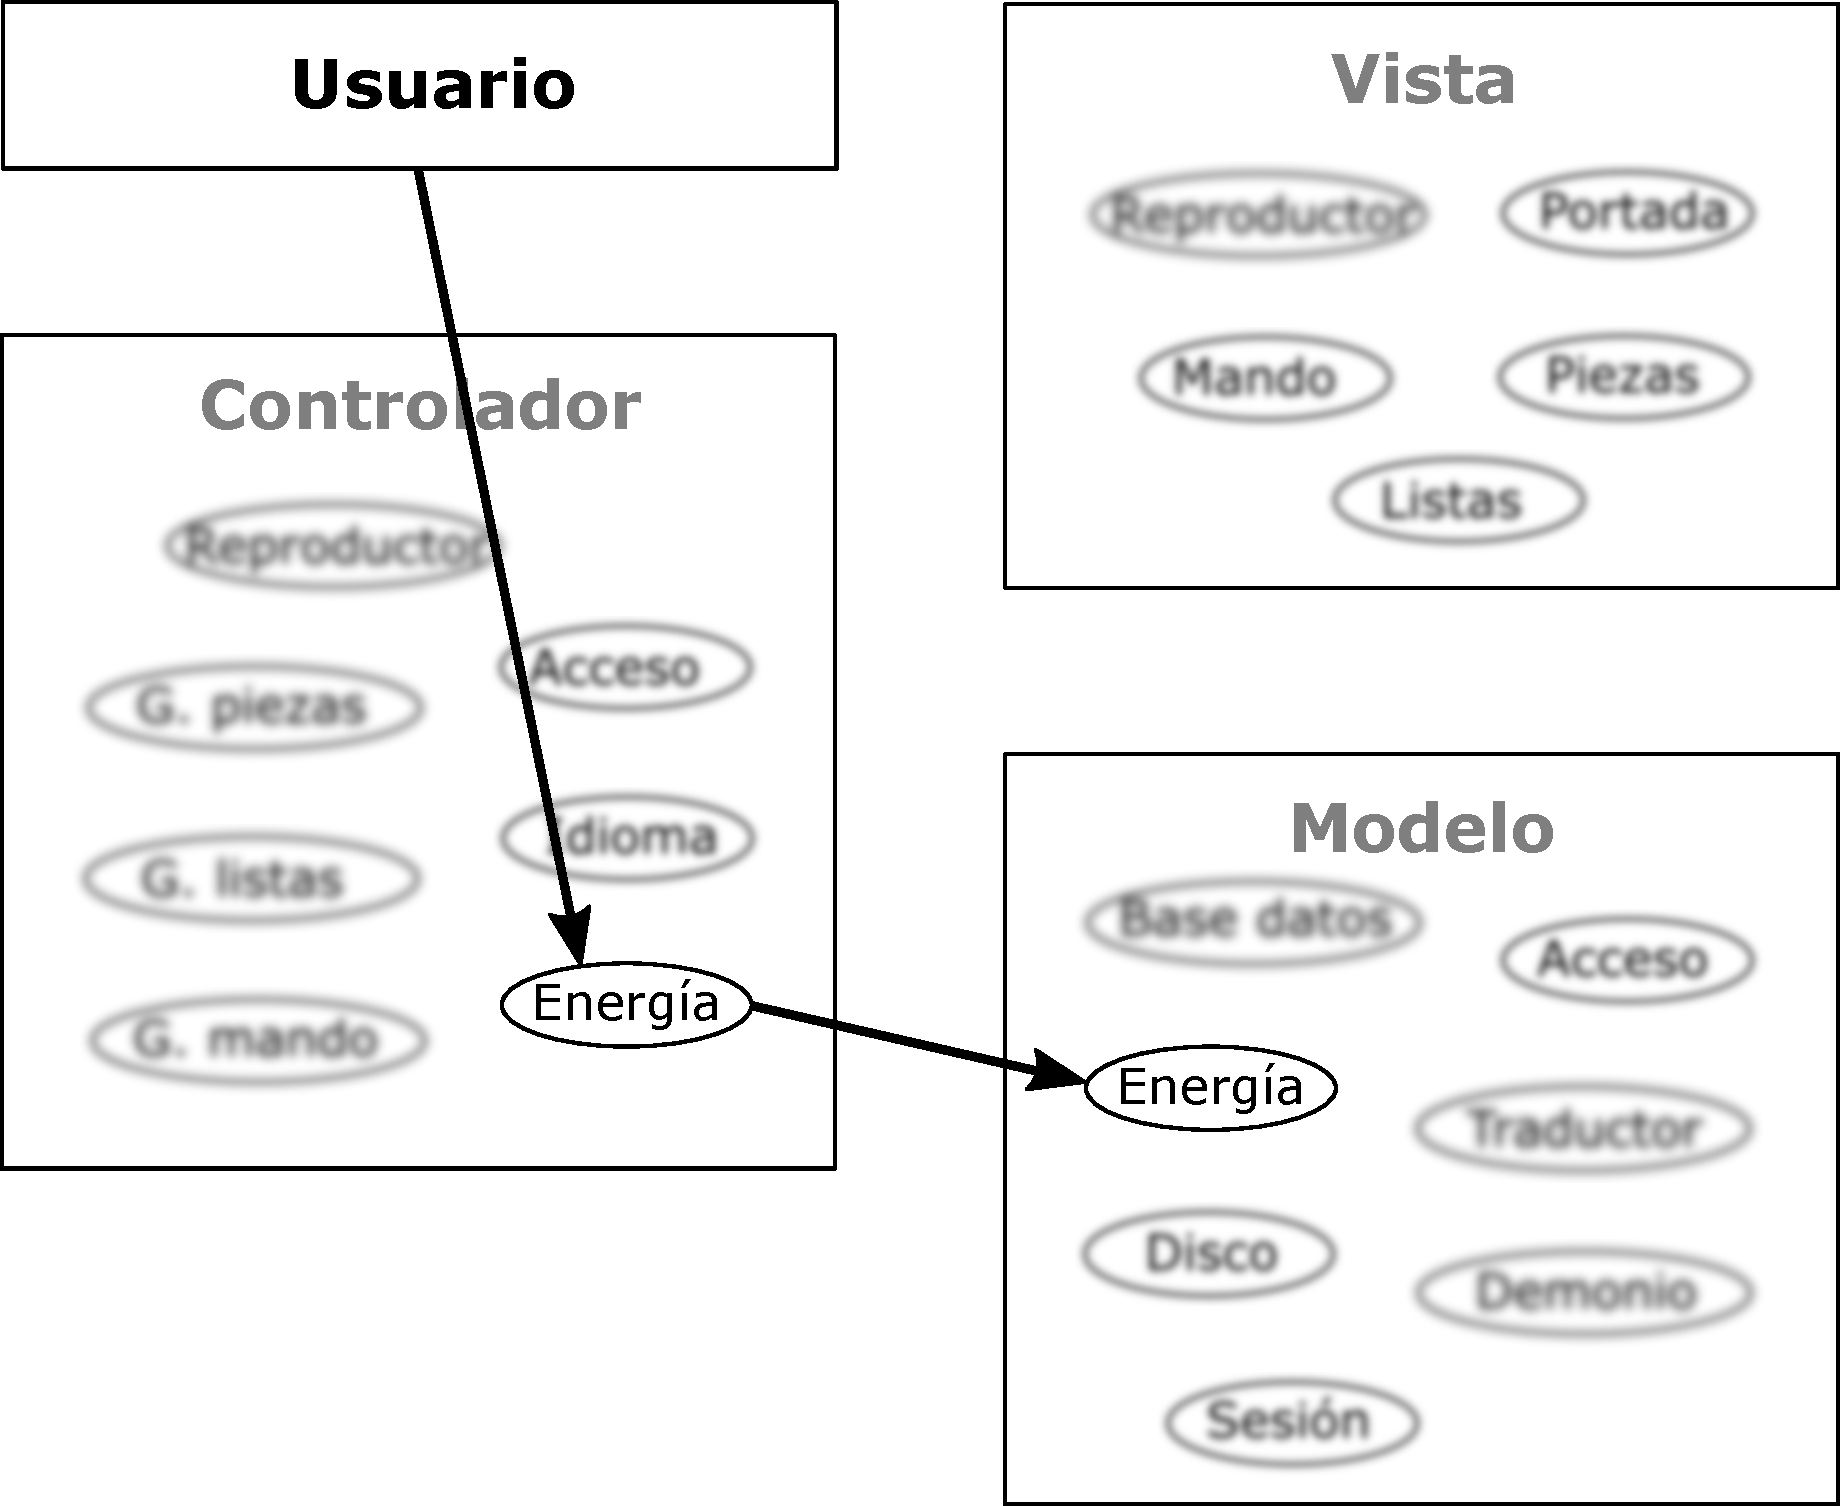
\includegraphics[width=\linewidth/2]{capitulo4/mvc_energia}
		\par\end{centering}
	\smallskip
	\caption{\label{fig:mvc_energia} Módulos implicados en el control de energía.}
\end{figure} 

\smallskip

\subsection{Soporte de idiomas}

Uno de los requisitos especificados es que la interfaz soporte varios idiomas. Modelaremos la solución para que sea fácil tanto escoger un idioma como agregar nuevas lenguas.

Para ello, utilizaremos archivos de traducción independientes que el sistema detectará automáticamente, permitiendo que añadir un idioma sea tan sencillo como agregar un fichero nuevo.

Al igual que el control de energía, el selector de idioma aparecerá como un menú desplegable en la cabecera de la aplicación, pero a diferencia de aquél, también se mostrará en la portada.

\subsubsection{Formato del archivo de traducción}

El sistema de traducción estará basado en pares \textit{clave-contenido}. El lenguaje de los ficheros derivará del \acrshort{XML} ---\textit{\acrlong{XML}}--- y tendrá la siguiente estructura:

\begin{description}[style=nextline]
	\item[translation]
	Elemento raíz. Define la traducción completa a un idioma. Sus atributos son:
	
	\begin{description}
		\item[code] Código estándar del idioma, como "es" (español) o "en" (inglés).
		\item[language] Nombre de la lengua, escrito en el propio idioma.
	\end{description}
	
	Contendrá como hijos tantos elementos \textit{string} como sea necesario.
	
	\item[string]
	Significado de una cadena clave. Tiene un atributo:
	
	\begin{description}
		\item[name] Clave de traducción.
	\end{description}
	
	Su nodo hijo será la cadena de texto que se mostrará en la interfaz.
\end{description}

\subsubsection{Diagrama de uso}

De la misma forma que ocurría con el gestor de energía, no existe una vista propia de este componente. Con lo cual solo tenemos elementos de modelo y de controlador:

\smallskip

\begin{figure}[H]
	\noindent \begin{centering}
		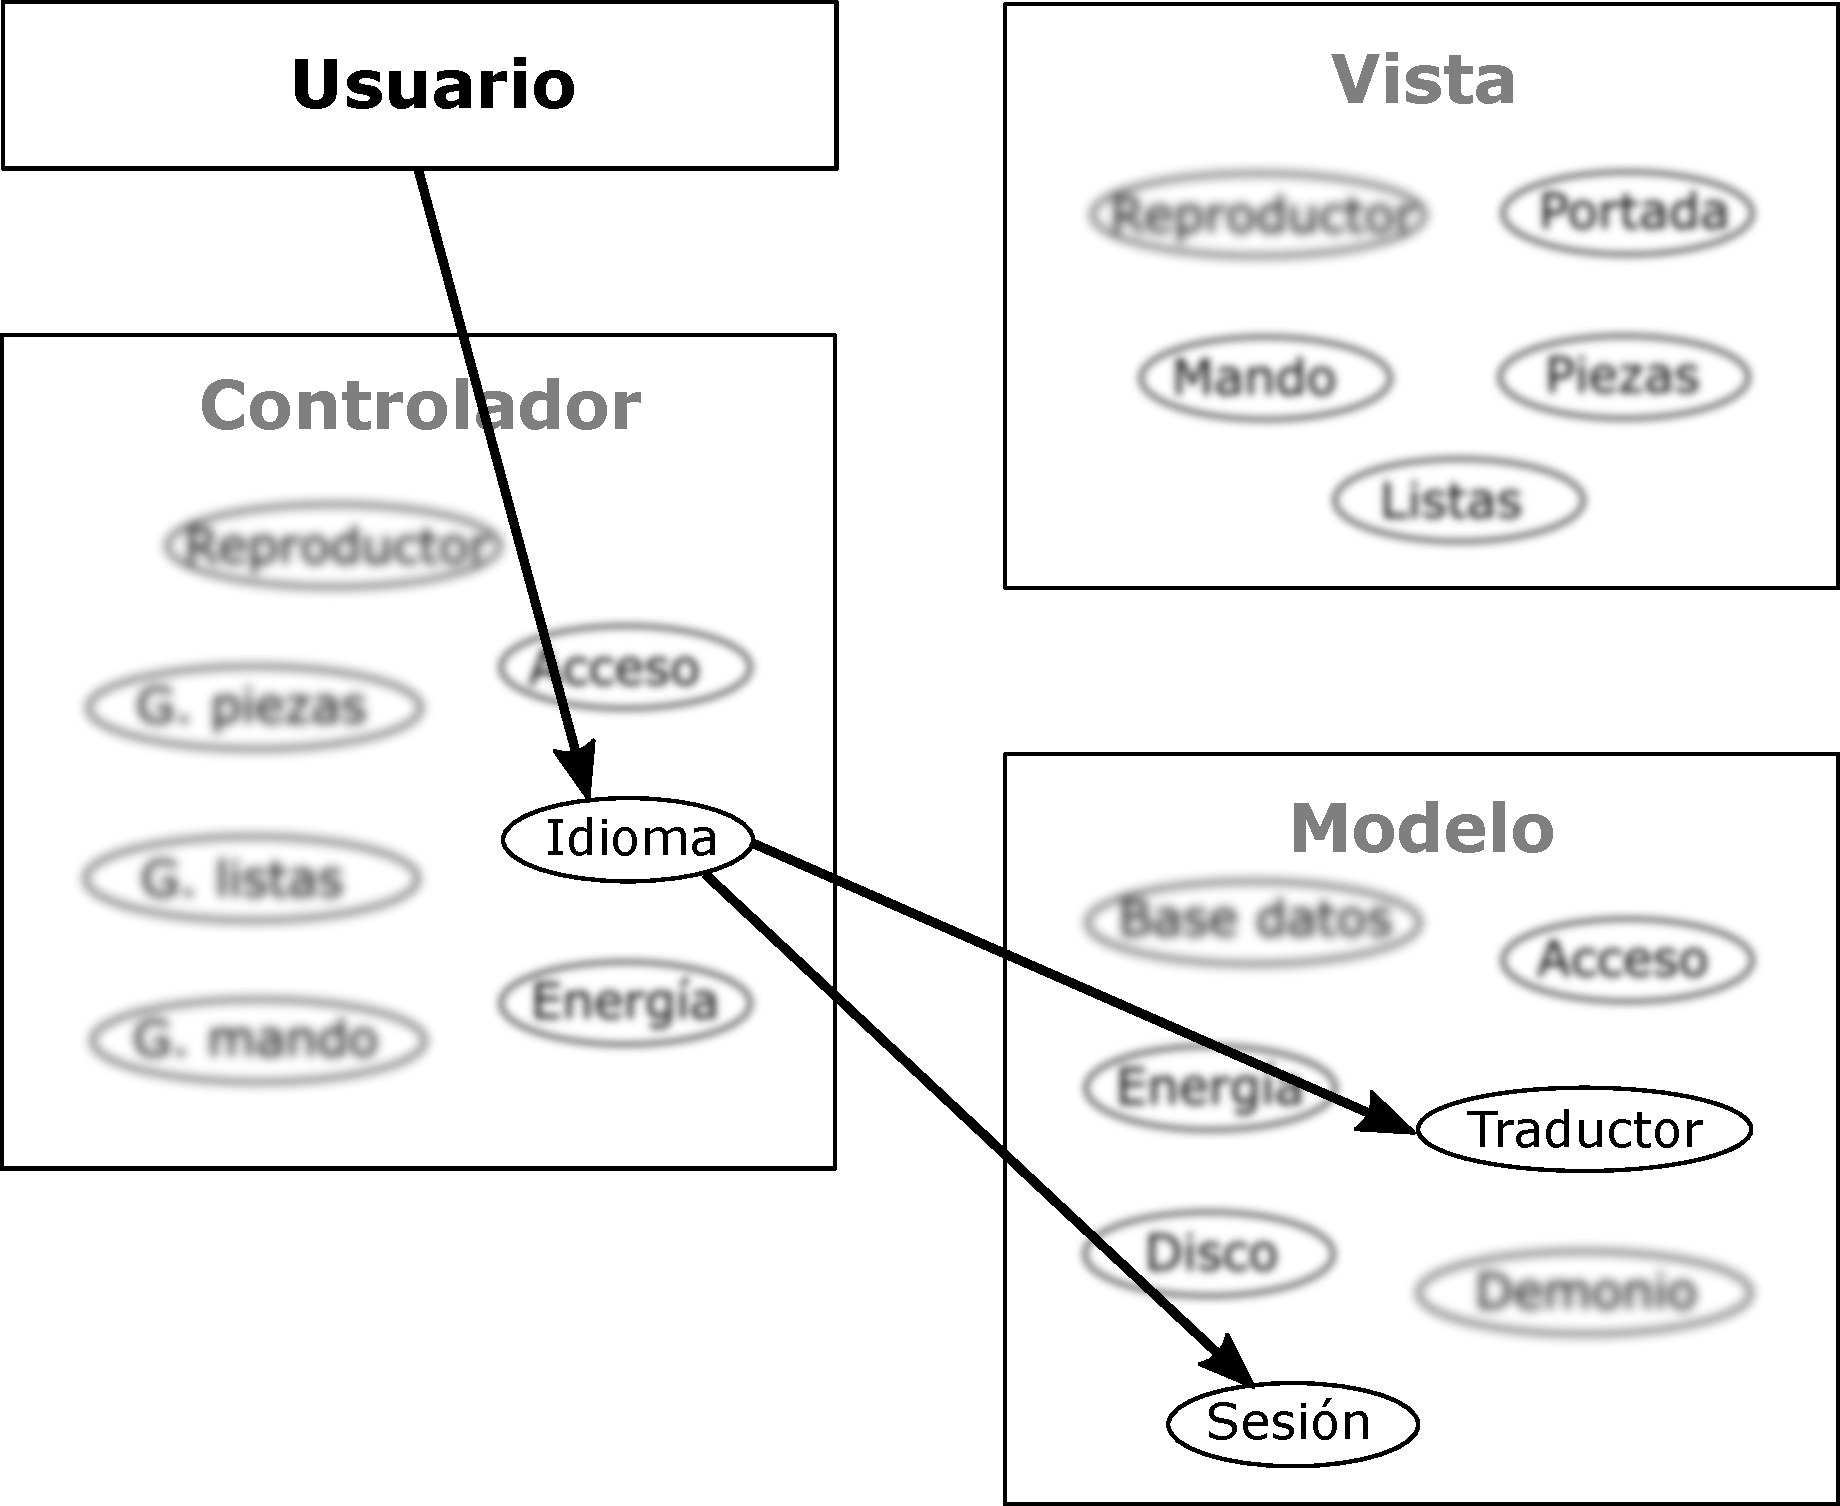
\includegraphics[width=\linewidth/2]{capitulo4/mvc_idioma}
		\par\end{centering}
	\smallskip
	\caption{\label{fig:mvc_idioma} Módulos implicados en el control de energía.}
\end{figure} 

\smallskip

\subsubsection{Funciones}

El módulo de traducción consta de los siguientes elementos:

\begin{description}[style=nextline]
	\item[Estructura \textit{Translator}]
	Representa un traductor, con los siguientes campos:
	
	\begin{description}
		\item[code] Código estándar del idioma.
		\item[language] Nombre de la lengua.
		\item[strings : \textit{array(string)}] Lista de cadenas de traducción.
	\end{description}
	
	\item[language (code)]
	Selecciona una lengua para la interfaz y almacena el código en la sesión.
	
	\begin{description}
		\item[code] Código del lenguaje, tal como aparece en el archivo de traducción.
	\end{description}
	
	Redirige a la vista que ha llamado al controlador.
	
	\item[translator ()]
	Pertenece al modelo. Busca y carga todos los archivos de traducción.
	
	\item[get\_translator (code)]
	Pertenece al modelo. Busca y obtiene un objeto traductor.
	
	\begin{description}
		\item[code] Código estándar del idioma.
	\end{description}
	
	Devuelve el objeto traductor indicado por el código.
\end{description}

\subsection{Navegación}

Como hemos visto en las maquetas, tendremos un menú lateral que nos permitirá acceder a las vistas principales de la interfaz. Aparte quedan la portada, a la que no se podrá volver ---a menos que se cierre la sesión, lo que reiniciaría la navegación--- y el gestor de piezas de una lista, al que se accederá a través del gestor general de listas.

El siguiente diagrama ilustra las principales posibilidades de navegación:

\smallskip

\begin{figure}[H]
	\noindent \begin{centering}
		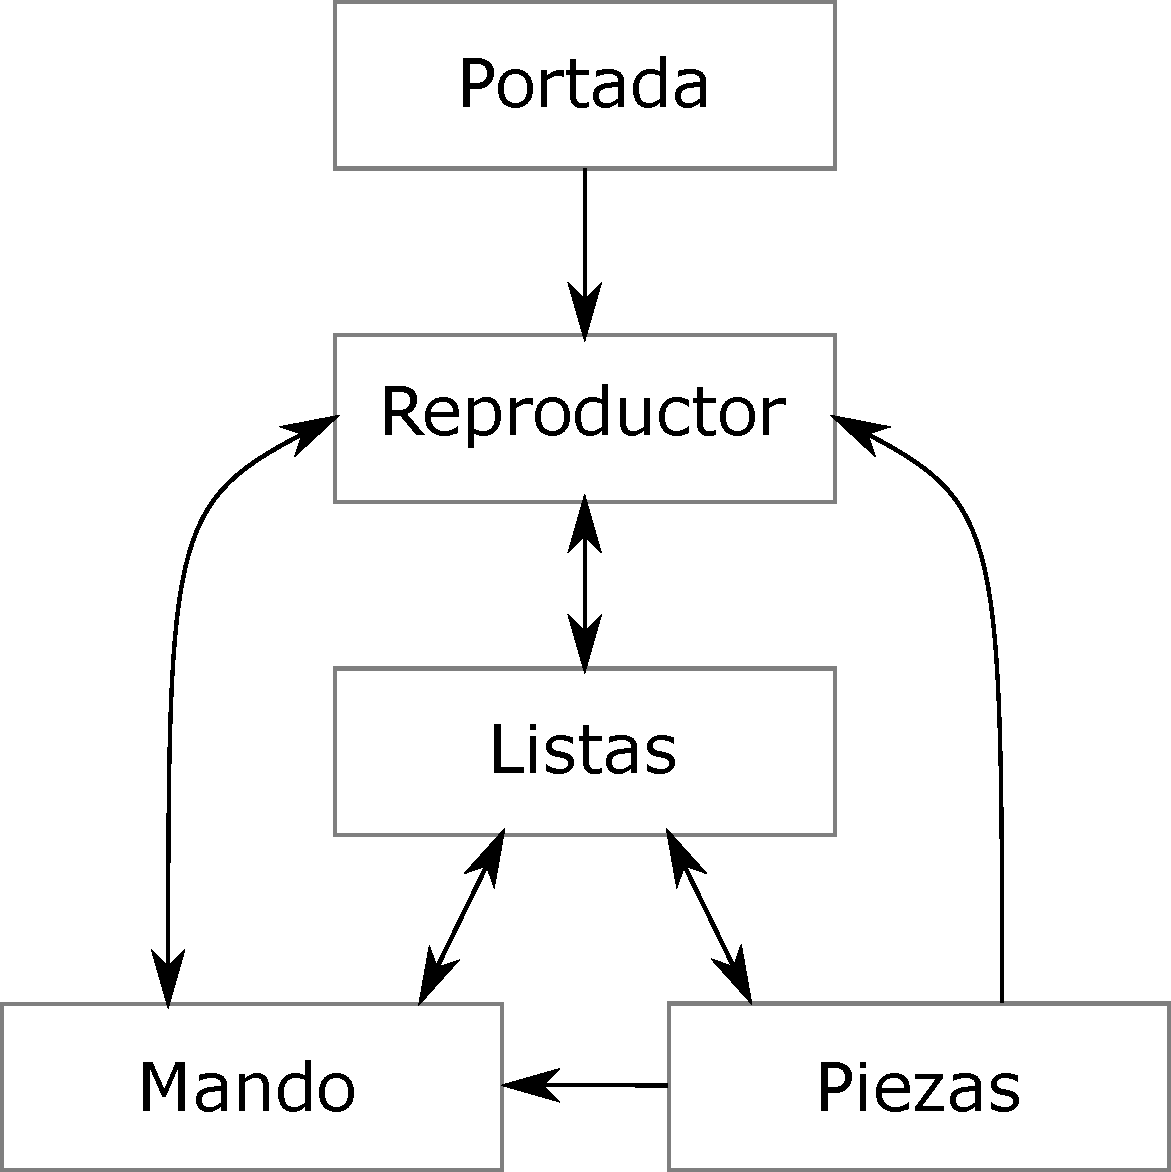
\includegraphics[width=\linewidth/2]{capitulo4/navegacion}
		\par\end{centering}
	\smallskip
	\caption{\label{fig:navegacion} Diagrama de navegabilidad entre vistas.}
\end{figure} 

\smallskip

\subsection{Sesión}

La comunicación entre servidor y cliente en un entorno \textit{web} utiliza el protocolo \acrshort{HTTP} (\textit{\acrlong{HTTP}}), un modelo de conexión sin estado ---\textit{stateless}---, una característica positiva en balance para este tipo de sistemas, pero nos limita a la hora de pretender una comunicación efectiva.

Para solventar este problema, almacenaremos en el servidor una pequeña cantidad de información relativa al cliente, tal como la que sigue:

\begin{enumerate}
	\item Marca de autentificación.
	\item Lenguaje que ha seleccionado para la interfaz.
	\item Última vista ejecutada, útil para ciertos controladores.
\end{enumerate}

En aras de promover un diseño limpio y extensible, aislaremos esta pequeña funcionalidad en un módulo aparte en el modelo, y que sea independiente del lenguaje de implementación.

\subsubsection{Funciones}

Las funciones del modelo dedicadas a manipular la sesión son las siguientes:

\begin{description}[style=nextline]
	\item[test\_auth ()]
	Comprueba si existe marca de autentificación. Si no la hay, redirige a la portada.
	
	\item[get\_auth () : \textit{boolean}]
	Devuelve si existe (\textit{true}) o no (\textit{false}) la marca de autentificación.
	
	\item[set\_auth ()]
	Establece la marca de autentificación. El usuario se acaba de identificar.
	
	\item[unset\_auth ()]
	Quita la marca de autentificación. El usuario acaba de cerrar la sesión.
	
	\item[set\_page (file)]
	Guarda el nombre de una página como la última vista ejecutada.
	
	\begin{description}
		\item[file] Nombre de la página.
	\end{description}
	
	\item[last\_page ()]
	Devuelve el nombre de la última página almacenada.
	
	\item[set\_language (code)]
	Establece el código de idioma como seleccionado por el usuario.
	
	 \begin{description}
	 	\item[code] Código estándar del idioma escogido.
	 \end{description}
	 
	 \item[get\_language ()]
	 Devuelve el código de lengua escogido por el usuario o, en su defecto, el código del idioma por defecto.
	
\end{description}

\subsection{Comunicación con el demonio}

Especificamos ahora el módulo que hará de modelo del servicio de reproducción, ofreciendo procedimientos para realizar las operaciones elementales sobre el reproductor. Se comunicará con el demonio a través del \textit{socket} local que implementa para tal efecto (véase el apartado \ref{subsec:daemon}), y utilizando el protocolo que describiremos en la sección \ref{sec:protocolo}.

\subsubsection{Funciones}

Como podremos ver, la interfaz de este componente actúa como tocón hacia las funciones que implementa el planificador, descrito en la sección \ref{subsec:planificador}.

\begin{description}[style=nextline]
	\item[driver ()]
	Establece la comunicación con el \textit{socket}. En caso de error, muestra un mensaje.
	
	\item[driver\_play (playlist, ifirst) : \textit{boolean}]
	Reproduce una lista de piezas en bucle.
	
	\begin{description}
		\item[playlist : \textit{array(string)}] Lista de nombres de archivo \acrshort{MIDI} a reproducir.
		\item[ifirst : \textit{integer}] Índice del primer archivo a ejecutar, que se pondrá a la cabeza de la lista.
	\end{description}
	
	Devuelve \textit{true} en caso de éxito o \textit{false} en caso de error.
	
	\item[driver\_pause () : \textit{boolean}]
	Pausa la reproducción, si estaba activa. Devuelve \textit{true} en caso de éxito o \textit{false} en caso de error.
	
	\item[driver\_resume () : \textit{boolean}]
	Reanuda la ejecución, si estaba pausada. Devuelve \textit{true} en caso de éxito o \textit{false} en caso de error.
	
	\item[driver\_stop () : \textit{boolean}]
	Detiene completamente la reproducción. Devuelve \textit{true} en caso de éxito o \textit{false} en caso de error.
	
	\item[driver\_status () : \textit{array}]
	Consulta el estado de reproducción, y si corresponde, el nombre de archivo que se está reproduciendo. Devuelve un \textit{array} de uno o dos elementos, dependiendo del estado:
	
	\begin{description}
		\item[PLAYING, <archivo>] Reproduciendo el archivo que indica (ruta absoluta).
		\item[PAUSED, <archivo>] Pausado sobre el archivo espeficicado (ruta absoluta).
		\item[STOPPED] Detenido.
		\item[ENGINEER] En modo Ingeniería. Cualquier orden será rechazada mientras se mantenga en este estado.
	\end{description}
	
\end{description}

\subsection{Comunicación con la base de datos}

La base de datos, diseñada en la sección \ref{sec:database}, es el principal nexo de unión entre el controlador y la vista. Aparte de las operaciones obvias, como insertar, modificar y eliminar partituras y listas, será utilizada al recibir el nombre de archivo que se está reproduciendo para inferir el título de la obra y la lista a la que pertenece.

Por otro lado, el controlador del mando realiza asignaciones de botones a listas, y esta información es recogida por el demonio, en el componente descrito en la sección \ref{subsec:daemon_mando}.

\subsubsection{Funciones}

La interfaz del modelo de la base de datos es la que sigue:

\begin{description}[style=nextline]
	\item[Estructura \textit{playlist}]
	Representa una lista de reproducción. Sus campos son:
	
	\begin{description}
		\item[id] Identificador único.
		\item[name] Nombre de la lista.
		\item[scores : \textit{array(score)}] Lista de partituras incluidas.
	\end{description}
	
	\item[Estructura \textit{score}]
	Representa una partitura musical. Incluye los siguientes atributos:
	
	\begin{description}
		\item[id] Identificador único.
		\item[name] Nombre de la lista.
		\item[duration] Duración de la pieza, en segundos.
		\item[source] Ruta del archivo asociado.
		\item[playlist] ID de la lista contenedora.
	\end{description}
	
	\item[Estructura \textit{shortcut}]
	Representa una asignación de botón a una lista. Sus campos son:
	
	\begin{description}
		\item[id] Identificador único del botón.
		\item[playlist] Identificador de la lista de reproducción.
	\end{description}
	
	\item[database ()]
	Inicializa el módulo, se debe llamar a esta función antes que cualquier otra de esta interfaz. En caso de error, emite un mensaje.
	
	\item[db\_get\_playlists () : \textit{array(playlist)}]
	Devuelve una lista de todas las listas existentes en la base de datos.
	
	\item[db\_insert\_playlist (name) : \textit{integer}]
	Inserta una nueva lista de reproducción.
	
	\begin{description}
		\item[name] Nombre asignado a la lista.
	\end{description}
	
	Devuelve el ID de la nueva lista.
	
	\item[db\_get\_playlist (idplaylist) : \textit{playlist}]
	Busca una lista por ID.
	
	\begin{description}
		\item[idplaylist] Identificador único de lista.
	\end{description}
	
	Devuelve la lista de reproducción, o un valor nulo si no se encuentra.
	
	\item[db\_rename\_playlist (idplaylist, name)]
	Cambia el nombre de una lista.
	
	\begin{description}
		\item[idplaylist] Identificador único de lista.
		\item[name] Nuevo nombre de la lista.
	\end{description}
	
	\item[db\_delete\_playlist (idplaylist)]
	Borra una lista de la base de datos.
	
	\begin{description}
		\item[idplaylist] Identificador único de lista.
	\end{description}
	
	\item[db\_insert\_score (idplaylist, name) : \textit{integer}]
	Inserta una nueva partitura en la base de datos, dentro de una lista de reproducción
	
	\begin{description}
		\item[idplaylist] Identificador único de la lista que contendrá a la pieza.
		\item[name] Título de la obra insertada.
	\end{description}
	
	Devuelve el ID de la pieza insertada.
	
	\item[db\_get\_score (idscore) : \textit{score}]
	Obtiene una partitura por ID.
	
	\begin{description}
		\item[idscore] Identificador único de pieza.
	\end{description}
	
	Devuelve la estructura \textit{score} correspondiente, o un valor nulo si no se encuentra.
	
	\item[db\_set\_score\_duration (idscore, duration)]
	Establece la duración de una pieza.
	
	\begin{description}
		\item[idscore] Identificador único de partitura.
		\item[duration] Duración de la pieza, en segundos.
	\end{description}
	
	\item[db\_find\_score (source) ]
	Busca una partitura por el nombre de archivo.
	
	\begin{description}
		\item[source] Nombre del archivo \acrshort{MIDI} como criterio de búsqueda.
	\end{description}
	
	Devuelve el objeto \textit{score} de la partitura, o un valor nulo si no se encuentra.
	
	\item[db\_rename\_score (idscore, name)]
	Cambia el nombre de una partitura.
	
	\begin{description}
		\item[idscore] Identificador único de pieza.
		\item[name] Nuevo título de la obra.
	\end{description}
	
	\item[db\_delete\_score (idscore)]
	Elimina la tupla correspondiente a una pieza.
	
	\begin{description}
		\item[idscore] Identificador único de partitura.
	\end{description}
	
	\item[db\_get\_shortcuts () : \textit{array(shortcut)}]
	Obtiene una lista con todas las asignaciones del mando a distancia.
	
	\item[db\_set\_shortcut (idshortcut, idplaylist)]
	Establece una asignación de un botón del mando a una lista de reproducción.

	\begin{description}
		\item[idshortcut] Identificador único del botón.
		\item[idplaylist] Identificador único de la lista.
	\end{description}
\end{description}

\section{Protocolo entre el control y el demonio}
\label{sec:protocolo}

Como hemos visto, la interfaz de usuario y el servicio en segundo plano se comunican a través de un socket que hace de puente entre el reproductor de la interfaz y el planificador del demonio.

La interfaz estará basada en lenguaje natural, su diseño debe ser sencillo y debe maximizar la coherencia entre ambos subsistemas, evitando inconsistencias en supuestos como los siguientes:

\begin{enumerate}
	\item El usuario hace una petición de reproducción e inmediatamente después se desconecta.
	\item Se elimina la lista de reproducción que se está ejecutando.
	\item Varios usuarios controlan simultáneamente la interfaz
\end{enumerate}

Para obtener una comunicación consistente, el demonio no guardará más estado que el del planificador, y no será consciente de la organización en listas de reproducción de la base de datos. Por su parte, la interfaz gráfica se referirá a las partituras con rutas absolutas a los archivos correspondientes a las partituras.

Las peticiones que describen el protocolo resultante, así como las posibles respuestas, se enumeran de la siguiente forma:

\begin{description}
	\item[PLAY <archivo> [ <archivo>*]] Reproducir una lista de archivos \acrshort{MIDI}, indicando las rutas completa, separadas por espacios. Respuesta:
	
	\begin{description}
		\item[OK] en caso de éxito.
		\item[ERROR] en caso de error o estar en modo Ingeniería.
	\end{description}
	
	\item[PLAYLOOP <archivo> [ <archivo>* ]] Reproducir en bucle una lista de archivos \acrshort{MIDI}, indicando las rutas completa, separadas por espacios. Respuesta:
	
	\begin{description}
		\item[OK] en caso de éxito.
		\item[ERROR] en caso de error o estar en modo Ingeniería.
	\end{description}
	
	\item[PAUSE] Pausar la reproducción. Silencia las notas pero manteniendo el estado. Respuesta:
	
	\begin{description}
		\item[OK] en caso de éxito.
		\item[ERROR] en caso de error, como estar detenido, o en modo Ingeniería.
	\end{description}
	
	\item[RESUME] Reanuda la reproducción en el punto en que se pausó. Respuesta:
	
	\begin{description}
		\item[OK] en caso de éxito.
		\item[ERROR] en caso de error, como no estar pausado, o en modo Ingeniería.
	\end{description}
	
	\item[STOP] Detiene completamente la reproducción y libera la lista de reproducción. Respuesta:
	
	\begin{description}
		\item[OK] en caso de éxito.
		\item[ERROR] en caso de error o estar en modo Ingeniería.
	\end{description}
	
	\item[STATUS] Consulta el estado del reproductor. Respuesta:
	
	\begin{description}
		\item[PLAYING <archivo>] Reproduciendo el archivo cuya ruta absoluta se especifica.
		\item[PAUSED <archivo>] Pausado en un punto del archivo cuya ruta se indica.
		\item[STOPPED] Detenido. Es el estado inicial.
		\item[ENGINEER] En modo Ingeniería. No se podrá reproducir nada hasta desbloquearse.
	\end{description}
	
\end{description}

\section{Aplicaciones auxiliares}

De acuerdo con los requisitos, hemos concebido el sistema como la conjunción de tres grandes bloques: la base de datos, el demonio como \textit{back-end} y la interfaz \textit{web} como \textit{front-end}. Sin embargo, tal como están diseñados, existe una dependencia mutua total, contraproducente para la fase de implementación, donde será necesario realizar pequeñas pruebas sobre el código que vayamos construyendo.

Para verificar el desarrollo, vamos a prever la necesidad de probar los módulos críticos del diseño, a saber:

\begin{enumerate}
	\item Descodificador de archivos \acrshort{MIDI}.
	\item Planificador.
	\item Interfaz de salida.
	\item Servidor \textit{socket}.
\end{enumerate}

\smallskip

\begin{figure}[H]
	\noindent \begin{centering}
		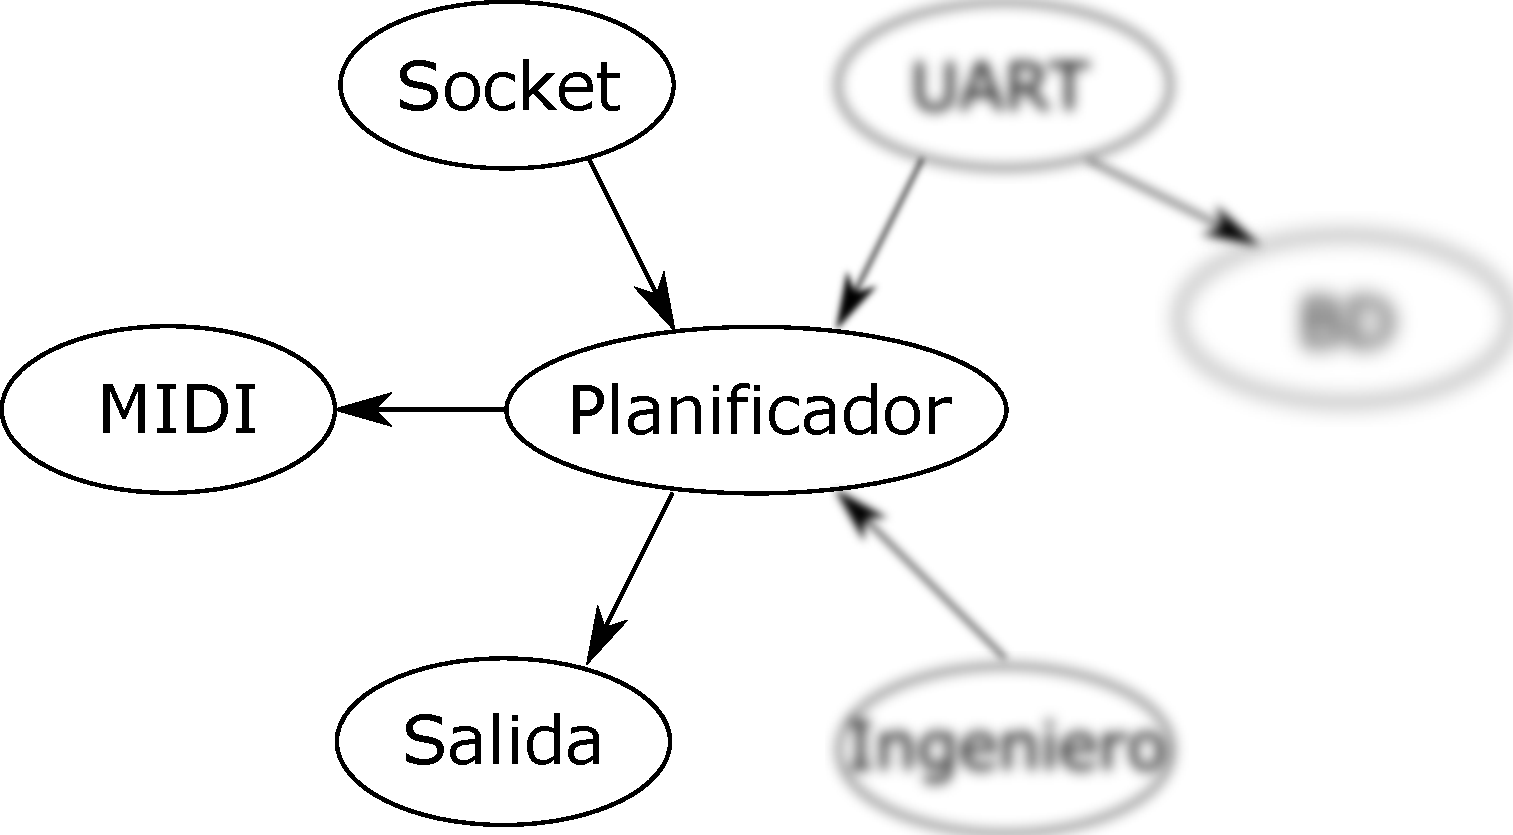
\includegraphics[width=\linewidth/2]{capitulo4/daemon_critical}
		\par\end{centering}
	\smallskip
	\caption{\label{fig:daemon_critical} Módulos críticos del back-end.}
\end{figure} 

\smallskip

En las secciones siguientes describiremos las soluciones que nos servirán para probar estos componentes.

Por otro lado, el \textit{front-end} necesita dos aplicaciones externas para distintos fines:

\begin{enumerate}
	\item El gestor de piezas (sección \ref{subsec:piezas}) requiere conocer la duración de una partitura mediante un programa que analice archivos \acrshort{MIDI}.
	\item El componente de autentificación (dentro de la sección \ref{subsec:portada}) necesita comprobar externamente la contraseña introducida por el usuario.
\end{enumerate}

\subsection{Información de archivo MIDI}
\label{subsec:midinfo}

Esta aplicación cumplirá dos fines:

\begin{enumerate}
	\item Validar el analizador de archivos \acrshort{MIDI}.
	\item Servir al \textit{front-end} la duración de una partitura.
\end{enumerate}

Sencillamente, utilizará la interfaz creada por el descodificador \acrshort{MIDI} (visto en la sección \ref{subsec:daemon_midi}) para enviar el nombre de un fichero \acrshort{MIDI}, descodificarlo y mostrar en la salida estándar la información básica de una partitura:

\begin{enumerate}
	\item Organización de las pistas.
	\item Número de pistas.
	\item División de tiempo.
	\item Duración de la obra.
\end{enumerate}

Esta información podrá ser aprovechada tanto desde el terminal como desde la interfaz gráfica.

\subsubsection{Diagrama de uso}

Al utilizar simplemente la interfaz del componente \acrshort{MIDI}, éste es el único elemento que habrá que implementar para validarlo.

\smallskip

\begin{figure}[H]
	\noindent \begin{centering}
		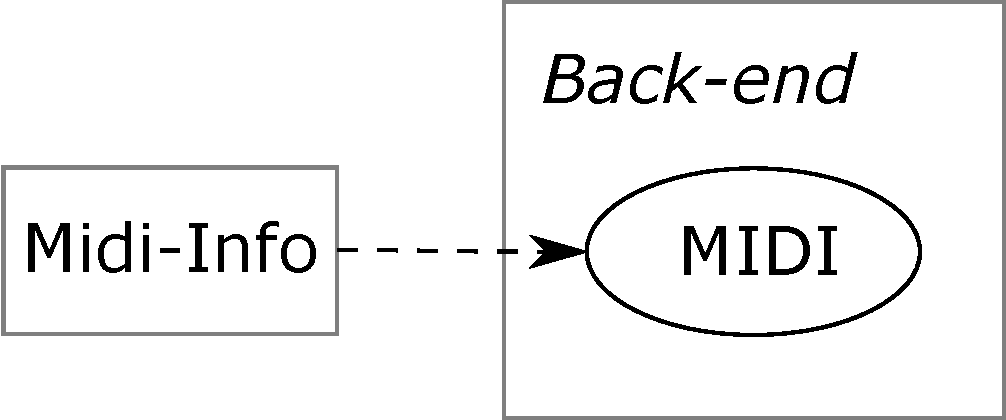
\includegraphics[width=\linewidth/3]{capitulo4/midi_info}
		\par\end{centering}
	\smallskip
	\caption{\label{fig:midi_info} Interacción del programa con el back-end.}
\end{figure} 

\smallskip

\subsection{Simulador de reproducción}

El siguiente bloque a construir será el planificador (véase la sección \ref{subsec:planificador}) y la interfaz de salida (explicada en la sección \ref{subsec:output}). Ésta es una parte fundamental del planificador pero, como ya explicamos, la colocamos en un componente aparte para permitir implementar la interfaz según nuestras necesidades, bien para movernos de un órgano a otro, o bien para definir otro tipo de salida.

Vamos a hacer una pequeña aplicación que nos permita verificar el funcionamiento del planificador y la interfaz de salida, de la siguiente manera:

\begin{enumerate}
	\item Interactuará directamente con el planificador, de la misma forma que hará el \textit{socket} o el \acrshort{UART}.
	\item Implementará la salida (diseñada para el \acrshort{GPIO}) sobre la salida estándar, suplantando a la \acrshort{PCB}.
\end{enumerate}

\subsubsection{Diagrama de uso}

Este programa utilizará el planificador e implementará la interfaz de salida:

\smallskip

\begin{figure}[H]
	\noindent \begin{centering}
		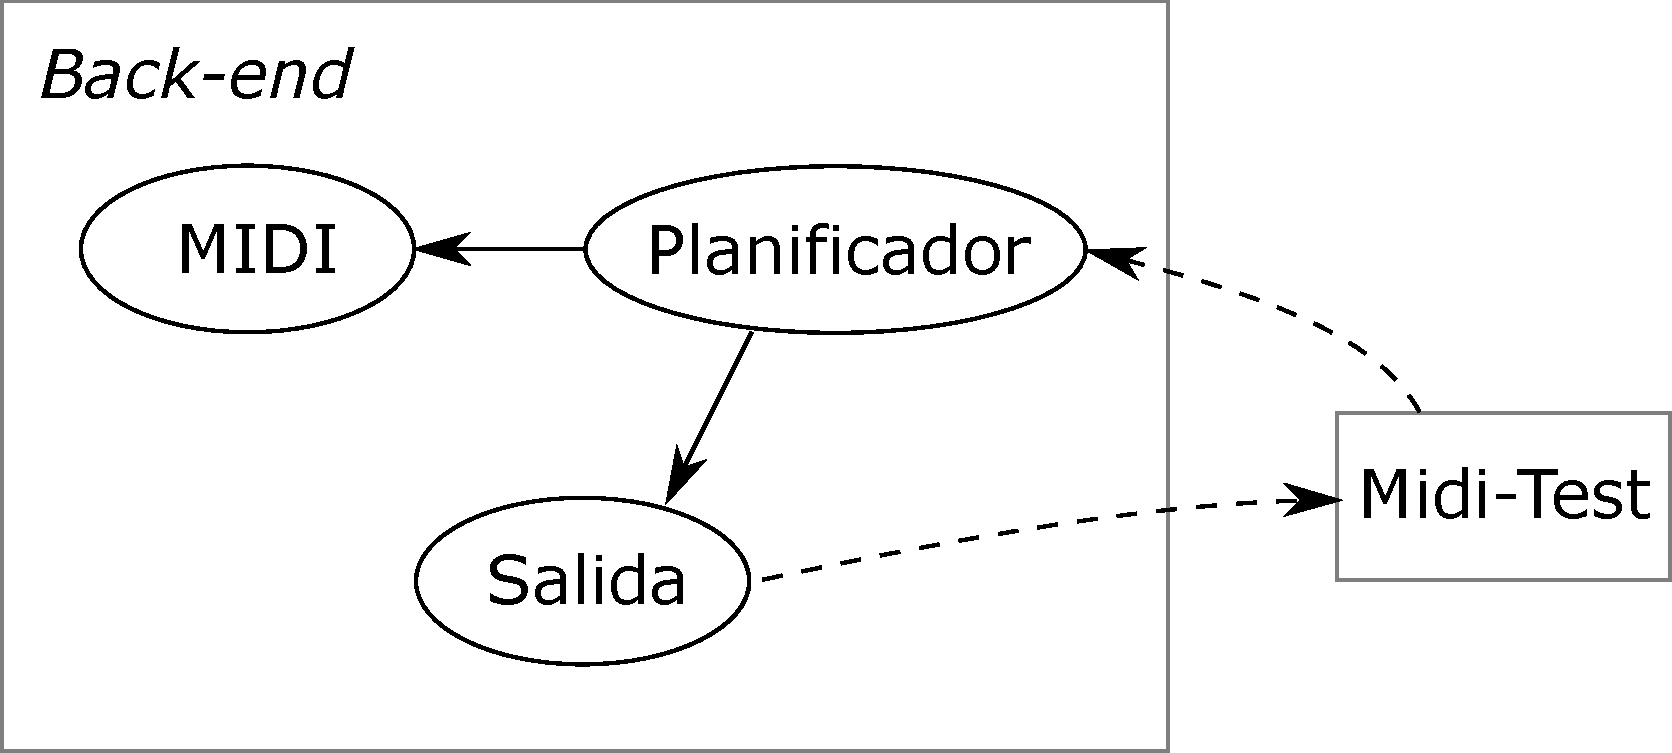
\includegraphics[width=\linewidth/2]{capitulo4/midi_test}
		\par\end{centering}
	\smallskip
	\caption{\label{fig:midi_test} Interacción del programa con el back-end.}
\end{figure} 

\smallskip

\subsection{Terminal del reproductor}

Una vez implementados los componentes críticos del demonio, crearemos un sencillo programa que haga las llamadas básicas del protocolo a través del \textit{socket}, como lo hará la interfaz gráfica. Esto nos permitirá comprobar que la estructura principal funciona correctamente, y manejar el reproductor sin la interfaz gráfica.

La aplicación admitirá los siguientes argumentos:

\begin{description}
	\item[play <archivo>] Ejecutar un fichero \acrshort{MIDI}.
	\item[playloop <archivo>] Reproducir en bucle un archivo..
	\item[pause] Pausar la reproducción, si estaba funcionando.
	\item[resume] Reanudar la ejecución, si estaba pausada.
	\item[stop] Detener completamente la reproducción.
	\item[status] Mostrar información del planificador.
\end{description}

\subsubsection{Diagrama de uso}

Contando con una etapa madura del desarrollo, el terminal se comunicará con el \textit{back-end} a través del socket. Esto requerirá que ya esté funcionando como proceso demonio, y permitirá detectar posibles errores de implementación.

\smallskip

\begin{figure}[H]
	\noindent \begin{centering}
		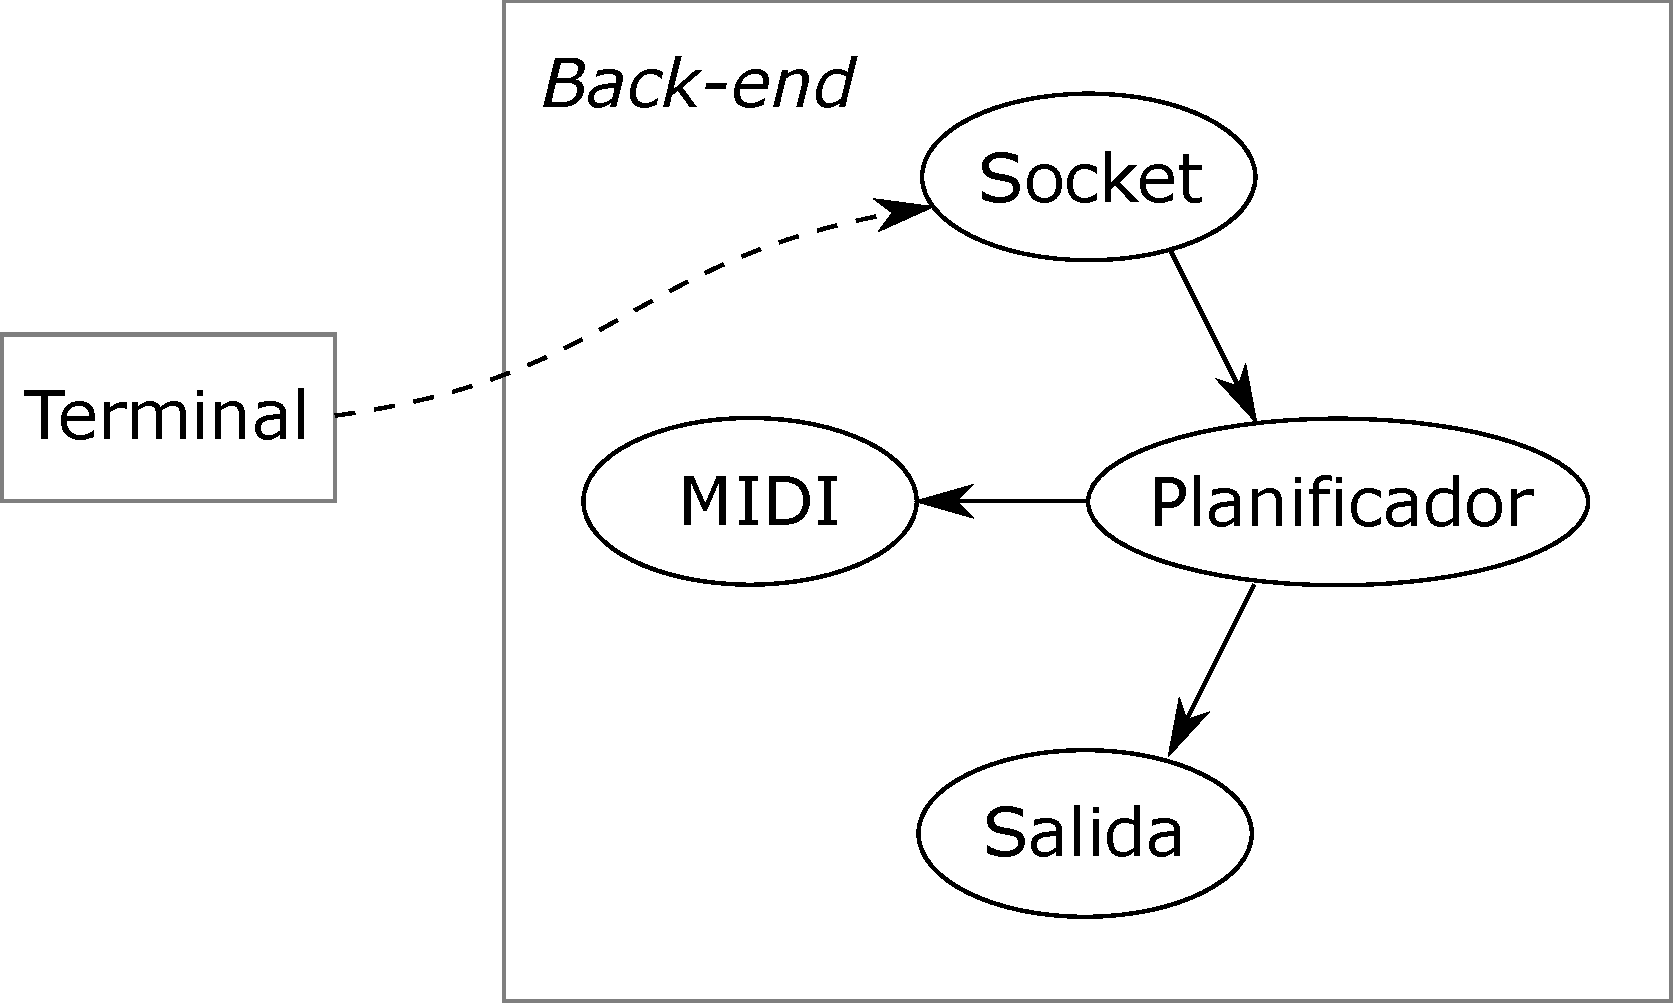
\includegraphics[width=\linewidth/2]{capitulo4/terminal}
		\par\end{centering}
	\smallskip
	\caption{\label{fig:terminal} Interacción del programa con el back-end.}
\end{figure} 

\smallskip

\subsection{Comprobación de contraseña}
\label{subsec:applogin}

Por último, concebiremos una aplicación minimalista para comprobar la contraseña del usuario. Dependiendo del grado de seguridad que implantemos, crearemos o no un usuario dedicado con permiso para utilizar la interfaz gráfica.

La aplicación recibe los siguientes argumentos por consola:

\begin{enumerate}
	\item Nombre de usuario.
	\item Contraseña introducida.
\end{enumerate}

Se verificará que la contraseña introducida corresponda a la del usuario en Linux con el nombre indicado, y el resultado se indicará como código de salida del proceso:

\begin{description}
	\item[0] Usuario y contraseña válidos.
	\item[1] El nombre de usuario no existe, o bien la contraseña es incorrecta.
\end{description}

\section{Resultado del diseño}

El desarrollo de este capítulo nos ha permitido afinar con un alto nivel de detalle el esbozo inicial (figura \ref{fig:idea}), hasta obtener los tres grandes bloques del diseño:

\begin{enumerate}
	\item Un demonio de Linux, como \textit{back-end}.
	\item Una base de datos, como sistema de almacenamiento persistente.
	\item Una interfaz \textit{web}, como \textit{front-end}.
\end{enumerate}

En definitiva, hemos concebido un completo sistema de control para la \acrshort{PCB}, cuyo funcionamiento se resume en el siguiente diagrama:

\smallskip

\begin{figure}[H]
	\noindent \begin{centering}
		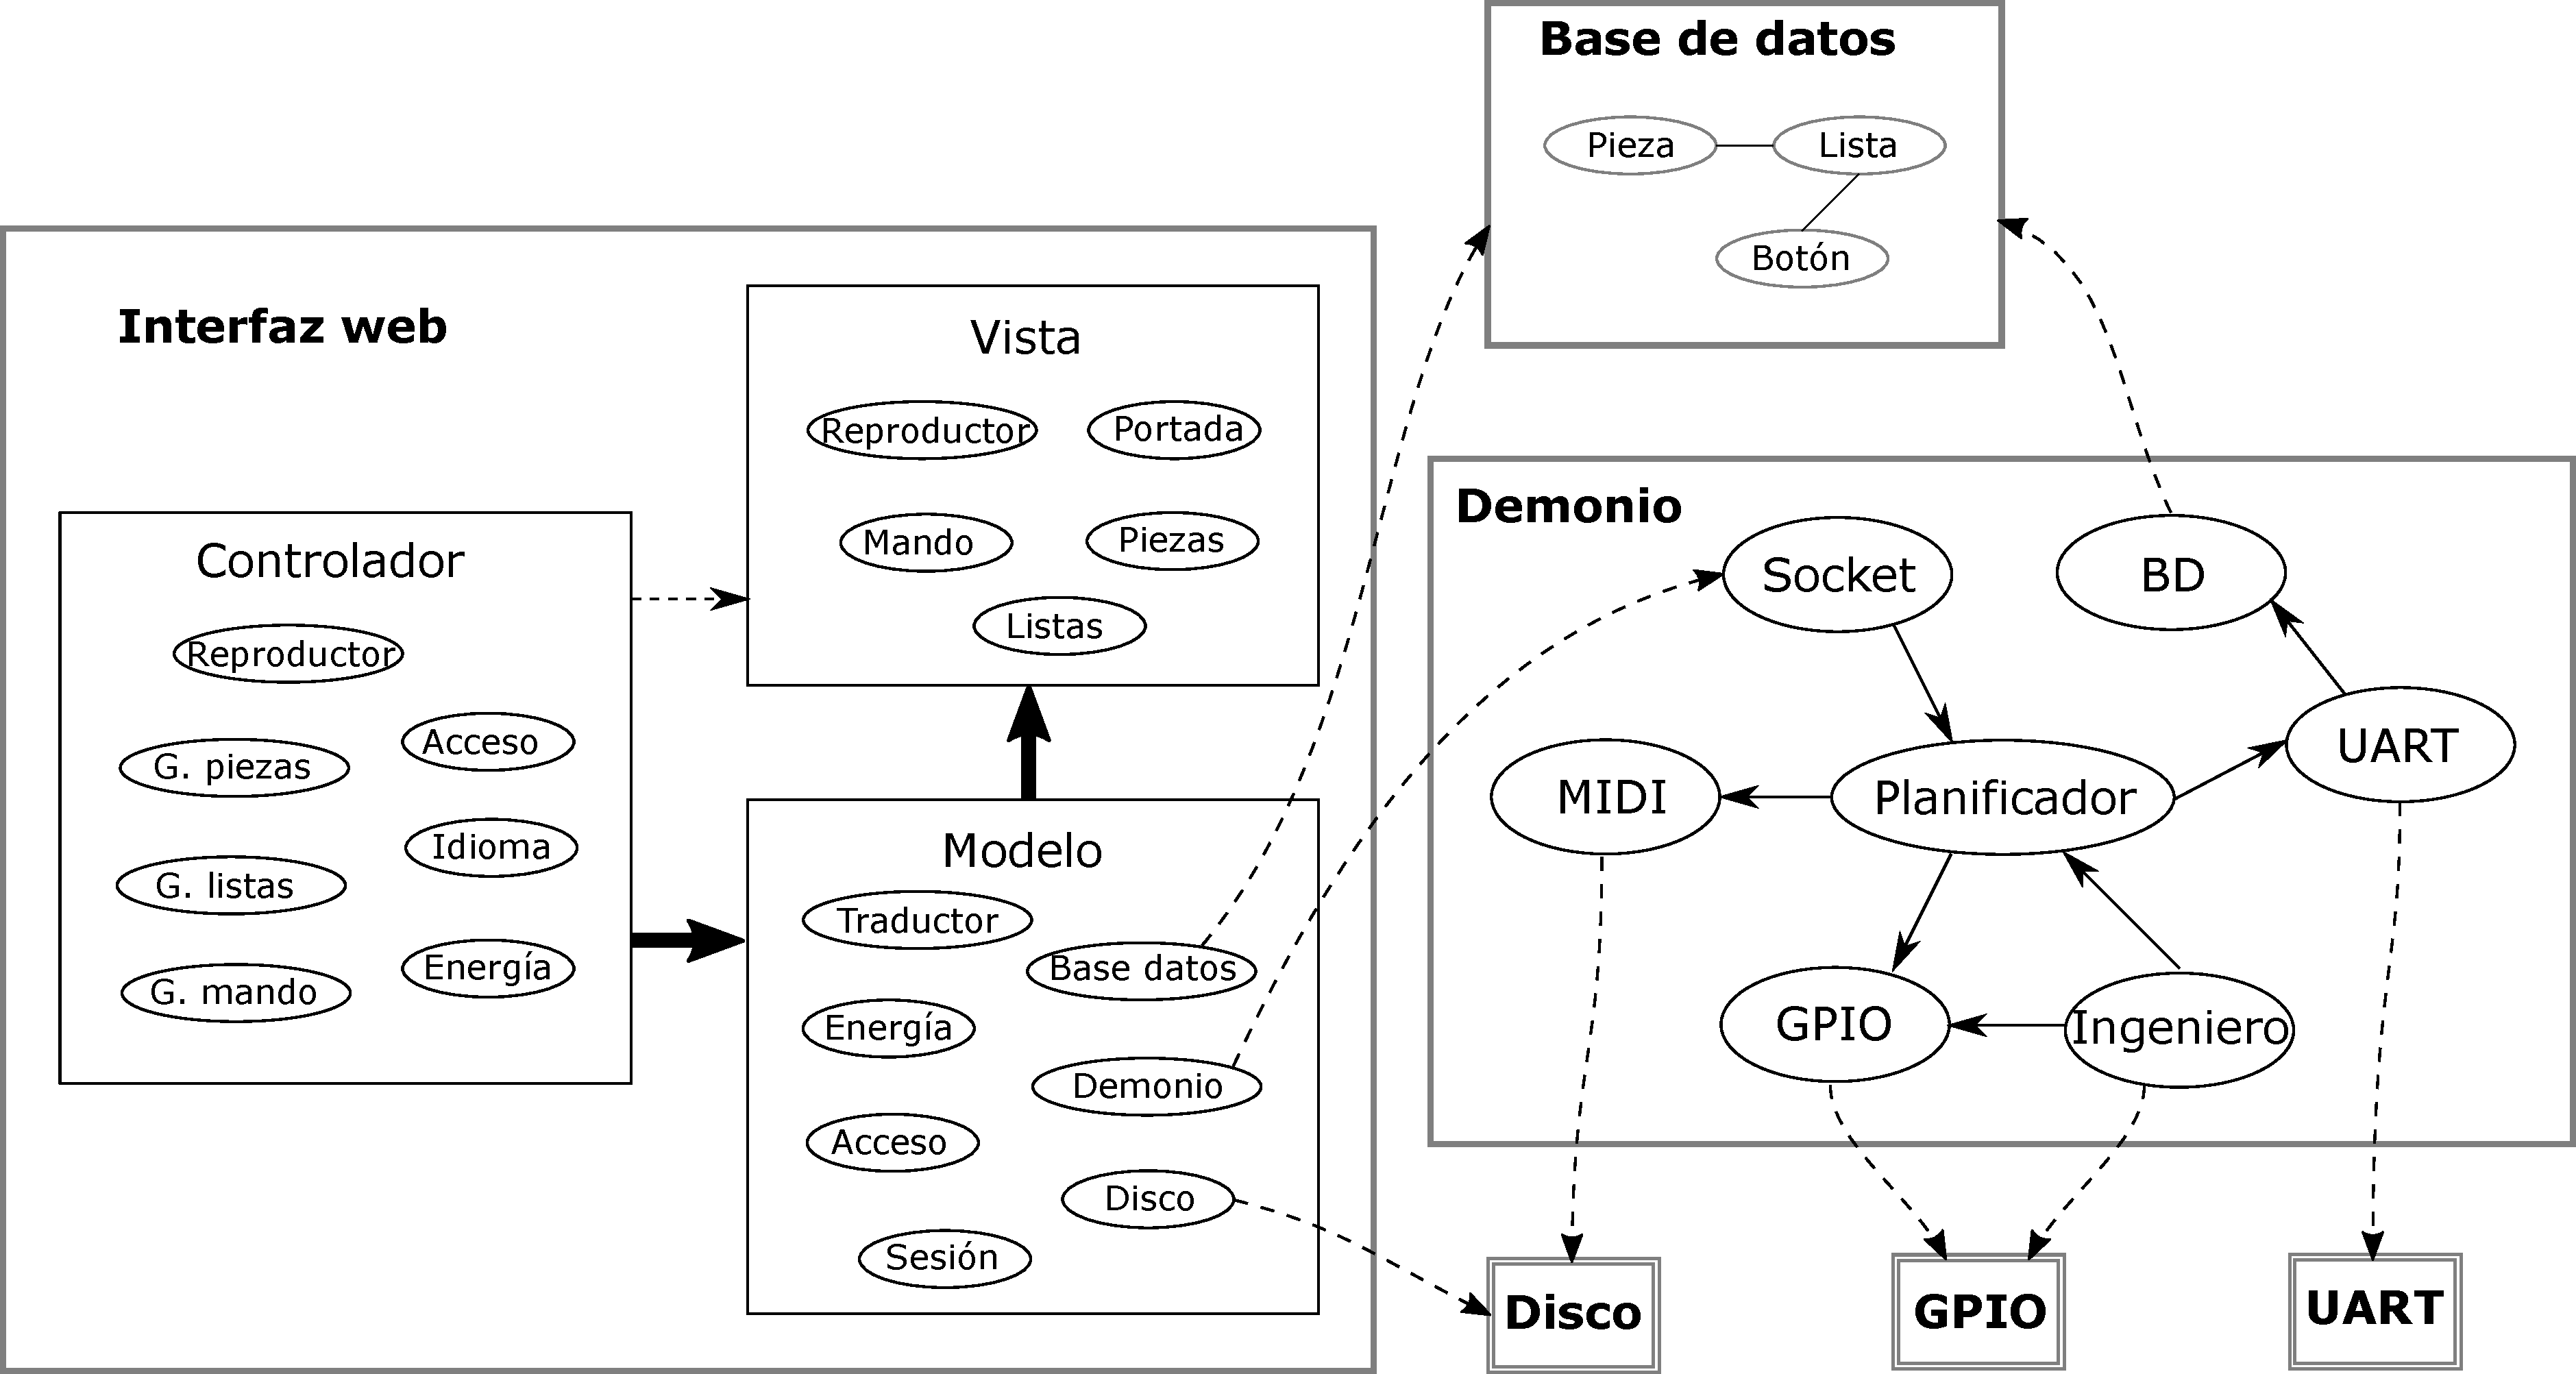
\includegraphics[width=\linewidth]{capitulo4/sistema}
		\par\end{centering}
	\smallskip
	\caption{\label{fig:sistema} Resumen del diseño del sistema.}
\end{figure} 

\smallskip

\clearpage{\cleardoublepage}
\clearpage{\pagestyle{empty}\cleardoublepage}